\documentclass[12pt]{book}
\usepackage{geometry}
\geometry{letterpaper, left=22.5mm, right=22.5mm, top=30mm, bottom=30mm}
\geometry{letterpaper}
\usepackage{amsmath}
\usepackage{amssymb}
\usepackage{enumitem}
\usepackage{fancyhdr}
\usepackage{framed}
\usepackage{tikz}
\usepackage{mathpazo}
%\usepackage{charter}
%\usepackage{newcent}
\usepackage{indentfirst}
\usepackage{booktabs}
\usepackage{graphicx}
\usepackage{float}
\usepackage{makecell}
\usepackage{xcolor}
\usepackage{mdframed}
\usetikzlibrary{trees}
\pagestyle{fancy}
\usepackage{amsthm}
\theoremstyle{definition}
\newtheorem{definition}{Definition}[section]
\theoremstyle{property}
\newtheorem{property}{Property}[section]
\theoremstyle{assumption}
\newtheorem{assumption}{Assumption}[section]
\theoremstyle{example}
\newtheorem{example}{Example}[section]
\theoremstyle{comment}
\newtheorem{comment}{Comment}[section]
\newtheorem{theorem}{Theorem}[section]
\newtheorem{corollary}{Corollary}[theorem]
\newtheorem{lemma}[theorem]{Lemma}
\usepackage{lastpage}
\usepackage{wrapfig}
\usepackage{hyperref}
\usepackage{subcaption}
\usepackage{setspace}
\usepackage{natbib}
\hypersetup{
colorlinks=true,
linkcolor=black,
filecolor=green, 
urlcolor=blue,
}
\newcommand{\ROM}[1]
    {\MakeUppercase{\romannumeral #1}}
\fancyhead[L]{Econometrics \ROM{2} }%change each reci
\fancyhead[R]{Spring 2020}
\fancyfoot[C]{\thepage \hspace{1pt} / \pageref{LastPage}}

    \newcommand{\prefacename}{Preface}
    \newenvironment{preface}{
        \vspace*{\stretch{2}}
        {\noindent \bfseries \Huge \prefacename}
        \begin{center}
            % \phantomsection \addcontentsline{toc}{chapter}{\prefacename} % enable this if you want to put the preface in the table of contents
            \thispagestyle{plain}
        \end{center}%
    }
    {\vspace*{\stretch{5}}}

\fancypagestyle{firstpage}{%
\fancyhf{}%
\renewcommand{\headrulewidth}{0mm}%
  \fancyfoot[C]{\thepage \hspace{1pt} / \pageref{LastPage}}
}
%change title each rec

\title{Introduction to Econometrics \ROM{2}: The Book\footnote{This book is meant to leave what was learned in the spring semester of the year 2020 as a record, hoping to help future first-year students navigate through the Econometrics sequence. I do not intend to publish this in any form. Thus, while sharing this file with others not necessarily affiliated to Columbia is allowed, I forbid reproducing this book for commercial purposes.}}
\date{Spring 2020 Semester}
\author{Seung-hun Lee\footnote{sl4436@columbia.edu. Contact me if you find any errors. }}


\begin{document}
\linespread{1.25}
\onehalfspacing
\maketitle
\pagestyle{empty}

\frontmatter
\pagenumbering{roman}

\begin{preface}
This `Book' is a compilation of all the recitation notes that I have used in the Spring 2020 semester when I worked as a teaching fellow for the Introduction to Econometrics \ROM{2} class at Columbia University. The intention behind The Book is to create a one-stop reference for all things that are related to graduate-level econometrics.  In particular, this book focuses on the following topics
\begin{enumerate}
\item Instrumental Variables
\item Generalized Method of Moments
\item Panel Data (both static and dynamic)
\item Bootstrapping and Multiple Tests
\item Quantile Regression
\item Nonparametric and Semiparametric Estimation
\item Program Evaluation and Treatment Effects: Random Assignment, Selection on Observables, Selection on Unobservables, and Regression Discontinuity
\item Introduction to Machine Learning
\end{enumerate}
\par
In creating this book, I have been indebted to many individuals. First, the contents are mainly based on the lecture notes of Professors Jushan Bai and Bernard Salanie. I was given a rare opportunity to go over the first-year material once more. With this opportunity, I was able to gain mastery of the relevant methods that I can take anywhere in my research career. I am grateful to both professors for giving me this chance. 
\par
I was also greatly helped by two individuals - Paul Sungwook Koh and Dong Woo Hahm. They provided me an access to their prevous recitation notes. I was able to refine my explanation based on their notes, which benefitted those who learned from me and myself. Without them, this teaching fellowship would have been monumenally difficult. 
\par
Last but not least, I thank the first year cohort of 2019-2020 academic year. Not only have they corrected mistakes in my notes as classes went on, but they also gave me constructive and positive feedbacks for the recitation notes that became this book. The motivation from these reviews helped me complete this work. 
\par
Any remaining errors - typos, concepts that could be explained more efficiently than stated, etc. - are mine. I would appreciate any comments regarding the errors you may find here. \par

\end{preface}

\tableofcontents



\mainmatter
\pagestyle{fancy}


%%%%%%%%%%%%%%%%%%

\chapter{Review on Asymptotic Theories}
\section{Motivation}
Econometrics is about drawing an empirical conclusion from the given data. In particular, we are interested in the features of the estimators that we obtain from the data. While we cannot be sure of the distribution of such estimators in a finite sample context, we can still use asymptotic theories to derive the approximate distribution. In particular, we are interested in the consistency and the asymptotic variance of an estimator. This is where various modes of convergence and related theorems come in handy. \par
Before moving on, here are the Markov Inequality and the Chevyshev Inequality that would serve useful in proving some key theorems on this note and throughout the semester. 
\begin{mdframed}[backgroundcolor=green!5] 
\begin{theorem}[Markov Inequality]
For any non-negative random variable $X$ and $\epsilon>0$,
\small{\[
\Pr(X\geq\epsilon)\leq\frac{E(X)}{\epsilon}
\] }\normalsize
\end{theorem}
\begin{theorem}[Chevyshev Inequality]
For any random variable $X$ and $\epsilon>0$, 
\small{\[
\Pr(|X-E(X)|\geq\epsilon)\leq\frac{var(X)}{\epsilon^2}
\] }\normalsize
\end{theorem}
\end{mdframed}\par
Another useful tool is the asymptotic notations, or what we know as ``Big $O$ and small $o$". The definitions and properties of each notations are as follows% Big O small o
\begin{mdframed}[backgroundcolor=blue!5] 
\begin{definition}[Asymptotic Notations]
A sequence of non-random vectors $X_n$ is said to be $O(1)$ if it is bounded and $o(1)$ if it converges to 0. In addition, if $a_n$ is a sequence of non-random positive scalars, we say $X_n$ is $O(a_n)$ if $\frac{X_n}{a_n}$ is bounded and $o(a_n)$ if $\frac{X_n}{a_n}\to0$
\end{definition}
\begin{definition}[Asymptotic Notations (Stochastic)]
A sequence of random vectors $X_n$ is $O_p(1)$ if it is bounded in probability\footnote{It means that for every $\epsilon>0$, there is a constant $M_\epsilon>0$ s.t. $\Pr(|X_n|>M_\epsilon)< \epsilon$ for all $n\in\mathbb{N}$} and $o_p(1)$ if it converges to zero in probability\footnote{Or for every $\epsilon>0$, $\Pr(|X_n|>\epsilon)\to0$}. If $a_n$ is a random variable, then $X_n$ is $O_p(a_n)$ if $\frac{X_n}{a_n}$ is $O_p(1)$. $X_n$ is $o_p(a_n)$ if $\frac{X_n}{a_n}\xrightarrow{p}0$.
\end{definition}
\begin{property}
The following holds true for $O_p$ and $o_p$
\small{\begin{enumerate}
\item $o_p(1)\implies O_p(1)$
\item If $X_n=O_p(a_n)$, then $X_n=o_p(b_n)$ for any $b_n$ s.t. $a_n/b_n\to0$
\item If random vector $X_n$ converges in distrubtion to $X$, Then $X_n=O_p(1)$
\item $o_p(1)+o_p(1)=o_p(1), O_p(1)+O_p(1)=O_p(1), o_p(1)+O_p(1)=O_p(1)$
\item $o_p(1)o_p(1)=o_p(1), O_p(1)O_p(1)=O_p(1), o_p(1)O_p(1)=o_p(1)$
\end{enumerate}}\normalsize
\end{property}
\end{mdframed} \par
\section{Various Modes of Convergence}
A minimal criterion of a good estimator is consistency, which tells us that some estimator $\hat{\theta}_n$ converges to a true value $\theta$ for sufficiently large $n$. Convergence in probability is used to analyze whether the estimator is consistent or not. 
\begin{mdframed}[backgroundcolor=blue!5] 
\begin{definition}[Convergence in Probability]
A sequence random variable $X_n\in \mathbb{R}$ \textbf{converges in probability} to a random variable $X$ if for any $\epsilon>0$, we have either one of 
\[
\lim_{n\to\infty}\Pr(|X_n-X|\leq\epsilon)=1 \ \text{or }\lim_{n\to\infty}\Pr(|X_n-X|>\epsilon)=0
\]
We denote this as $X_n\xrightarrow{p}X$. 
\end{definition}
\end{mdframed} \par
The estimator $\hat{\theta}_n$ is consistent if $\hat{\theta}_n\xrightarrow{p}\theta$. To show, consistency, we rely on the Weak Law of Large Numbers (hereafter WLLN). 
\begin{mdframed}[backgroundcolor=green!5] 
\begin{theorem}[WLLN] Let $\{X_n|n\geq1\}$ be a sequence of IID random variables with $E|X|<\infty$. Define $\bar{X}_n=\frac{1}{n}\sum_{i=1}^nX_i$, $\mu=E[X_1]$. Then, $\bar{X}_n\xrightarrow{p}\mu$. 
\begin{proof}
For simplicity, I work with the case where the variance of the random variables are finite, namely $var(X_1)=\sigma^2<\infty$. For any $\epsilon>0$, 
\[
\begin{aligned}
\Pr(|\bar{X}_n-\mu|>\epsilon)&\leq\frac{E(|\bar{X}_n-\mu|^2)}{\epsilon^2} \ (\because \text{Chevyshev})\\
&=\frac{\sigma^2}{n\epsilon^2} \ (\because\text{Sample variance of $X_n$}=\sigma^2/n)
\end{aligned}
\]
By taking $n\to\infty$, $\frac{\sigma^2}{n\epsilon^2}\to0$. Therefore, $\lim_{n\to\infty}\Pr(|\bar{X}_n-\mu|>\epsilon)=0$
\end{proof}
\end{theorem}
\end{mdframed}\par
We are also interested in the asymptotic distribution of the estimator. In particular, we are interested in checking whether the estimator is asymptotically normal. 
\begin{mdframed}[backgroundcolor=blue!5] 
\begin{definition}[Convergence in Distribution]
Let $X_n$ be a sequence of random variables with distribution $F_n(x)=\Pr(X_n\leq x)$. Let $X$ be a random variable whose distribution is $F(x)=\Pr(X\leq x)$. A sequence random variable $X_n\in \mathbb{R}$ \textbf{converges in distribution} to a random variable $X$ if at all $x$ at which $F(x)$ is continuous, 
\[
\Pr(X_n\leq x)\to \Pr(X\leq x)
\]
We denote this as $X_n\xrightarrow{d}X$. 
\end{definition}
\end{mdframed}\par
In words, $X_n\xrightarrow{d}X$ does not necessarily mean that $X_n$ and $X$ are close - but their CDFs are close. If $X_n\xrightarrow{p}X$, $X_n$ and $X$ are close. Therefore, convergence in distribution has a weaker requirement than convergence in probability.\par
Convergence in distribution is applied when we use a central limit theorem. 
\begin{mdframed}[backgroundcolor=green!5] 
\begin{theorem}[Lindberg-Levy CLT]
If $\{X_n|n\geq1\}$ is a sequence of IID random variables with $E(X_1)=\mu<\infty, var(X_1)=\sigma^2<\infty$, then
\footnotesize{\[
\sqrt{n}(\bar{X}_n-\mu)=\frac{1}{\sqrt{n}}\sum_{i=1}^n(X_i-\mu)\xrightarrow{d}N(0,\sigma^2) 
\]}\normalsize or in standardized notation,
\footnotesize{\[
\sqrt{n}\left(\frac{\bar{X}_n-\mu}{\sigma}\right)=\frac{1}{\sqrt{n}}\sum_{i=1}^n\left(\frac{X_i-\mu}{\sigma}\right)\xrightarrow{d}N(0,1) 
\]}\normalsize
\end{theorem}
\end{mdframed}
\par
To answer whether the approximation provided by the CLT is accurate, we refer to the Berry-Esseen Theorem.
\begin{mdframed}[backgroundcolor=green!5] 
\begin{theorem}[Berry-Esseen Theorem]
For all sample sizes $n$ and for all $t\in\mathbb{R}$, 
\footnotesize{\[
\left|\Pr\left(\sqrt{n}\frac{\bar{X}_n-\mu}{\sigma}\leq t\right)-\Phi(t)\right|<\frac{C\times E(|X_i-\mu|^3)}{\sigma^3\sqrt{n}}
\]}\normalsize
where the estimate of $C$ has changed over time: $C\in(0.4097, 0,4748)$. 
\end{theorem}
\end{mdframed}\par
The key advancement of this theorem is that it contains some implication about the rate of a convergence of a probability distribution of a random sample to a normal distribution. It also implies that the accuracy depends on the standardized absolute third moment of the distribution of $X_i, \frac{E(|X_i-\mu|^3)}{\sigma^3}$, and sample size. \par
We can extend the CLT to a multi-variate setting using Cramer-Wold Device.\par
\begin{mdframed}[backgroundcolor=green!5] 
\begin{theorem}[Cramer-Wold Device]
Let $X_n$ and $X$ be random vector in $\mathbb{R}^k$. Then, 
\[
X_n\xrightarrow{d}X\iff\lambda'X_n\xrightarrow{d}\lambda'X, \ \ \forall\lambda\in\mathbb{R}^k
\]
\end{theorem}

\begin{theorem}[Multivariate Lindberg-Levy CLT]
Let $X_1,..,X_n\in\mathbb{R}^k$ be IID and $E|| X_1||^2<\infty$. Then, as $n\to\infty$, 
\[
\sqrt{n}(\bar{X}_n-\mu)\xrightarrow{d}N(0,E[(X-\mu)(X-\mu)'])
\]
where $X\in\mathbb{R}^k$.
\begin{proof}
Since $X_i$ is IID, and $\lambda\in\mathbb{R}^k$, $\lambda'X_i$ is also IID, where $E[\lambda'X_i]=\lambda'\mu$ and $var(\lambda'X_i)=\lambda'var(X_i)\lambda$. By Lindberg-Levy CLT (scalar version), we can get
\[
\sqrt{n}(\lambda'\bar{X}_n-\lambda'\mu)\xrightarrow{d}N(0,\lambda'var(X_i)\lambda) \iff \lambda'(\sqrt{n}(\bar{X}_n-\mu))\xrightarrow{d} \lambda'(N(0,var(X_i)))
\]
Then, apply Cramer-Wold device to get $\sqrt{n}(\bar{X}_n-\mu)\xrightarrow{d}N(0,var(X_i))$
\end{proof}
\end{theorem}
\end{mdframed}\par


\section{Some Useful Theorems}
To get the distribution and check for consistency of a seemingly complicated estimators, we can use the following theorems. 
\begin{mdframed}[backgroundcolor=green!5] 

\begin{theorem}[Continuous Mapping Theorem]
If $X_n\xrightarrow{p,d}X$ as $n\to\infty$ and $g:\mathbb{R}^k\to\mathbb{R}^m$ is continuous at every point of a set $C$ s.t. $P(X\in C)=1$ (or $g$  has the set of discontinuity points $D$ s.t. $\Pr(X\in D)=0$), then
\[
g(X_n)\xrightarrow{p,d}g(X)
\]
\end{theorem}

\begin{theorem}[Slutsky's Theorem]
If $X_n\xrightarrow{d}X$ and $Y_n\xrightarrow{p}c$ ($c\in\mathbb{R}$) as $n\to\infty$
\begin{enumerate}
\item $X_n \pm Y_n \xrightarrow{d} X\pm c$
\item $X_nY_n \xrightarrow{d}Xc$
\item $\frac{X_n}{Y_n}\xrightarrow{d} \frac{X}{c}$, provided that $c\neq0$
\end{enumerate}
If $X_n\xrightarrow{p}X, Y_n\xrightarrow{p}Y$, then the following holds
\begin{enumerate}
\item $X_n \pm Y_n \xrightarrow{p} X\pm Y$
\item $X_nY_n \xrightarrow{p}XY$
\item $\frac{X_n}{Y_n}\xrightarrow{p} \frac{X}{Y}$, provided that $\Pr(Y=0)=0$
\end{enumerate}
\end{theorem}
\end{mdframed}\par
However, the Slutsky's Theorem does not work well when both random variables converge in distribution, but not in probability. For such cases, we need to consider whether the two different random variables JOINTLY converge to another vector of random variable. \par
\begin{mdframed}[backgroundcolor=yellow!5] 

\begin{example}[Counter-example]
Let $Z_n\xrightarrow{d}Z$, where $Z\sim N(0,1)$. Also define $Y_n = (-1)^nZ_n$. Then, $Y_n\xrightarrow{d} N(0,1)$ as well. However, $Z_n+Y_n$ displays following patterns
\small{\[
Z_n+Y_n = \begin{cases} 2Z_n & n\text{ being even} \\ 0& n\text{ being odd}\end{cases}
\]}\normalsize
Thus, for even numbered $n$, the distribution converges to $N(0,4)$. For odd numbered $n$, it converges to a distribution centered at 0. Therefore, $X_n+Y_n$ fails to converge in distribution to $2N(0,1)=N(0,4)$
\end{example}
\begin{example}[Relationship between convergence of marginal and joint distribution]
Suppose $\mathbf{X}_n=( A_n\  B_n)'$ and $\mathbf{X}=( A\ B)'$, where $A_n, B_n, A, B$ are random variables. 
\begin{itemize}
\item Suppose that $\mathbf{X}_n\xrightarrow{d} \mathbf{X}$.  From Cramer-Wold Device, let $\lambda=(1 \ 0)'$. By applying Cramer-Wold Device, we can obtain that $A_n\xrightarrow{d}A$. We can obtain similar results for $B_n\xrightarrow{d}B$. 
\item Convergence in distribution for marginal distributions does not imply the same for joint distribution. Let $A_n$ and $B_n$ be independent standard normal random variables for all $n$. Thus, $A_n,B_n\xrightarrow{d}Z\sim N(0,1)$ individually. Jointly, however, $(A_n \ B_n)'$ is bivariate normal with correlation 0 while $(Z \ Z)'$ is bivariate normal with correlation 1. Therefore, we cannot say $(A_n \ B_n)'$ converges in distribution to $(Z \ Z)'$
\item However, if it is the case that $A_n\xrightarrow{d}A$ and $B_n\xrightarrow{d}B$, where $A_n$ is independent of $B_n$ for all $n$ and $A$ is independent of $B$, it can be said that $\mathbf{X}_n\xrightarrow{d}\mathbf{X}$. This is because
\small{\[
F_{A_n,B_n}(a,b)=F_{A_n}(a)F_{B_n}(b)\to F_A(a)F_B(b)=F_{A,B}(a,b)
\]}\normalsize for all $a,b$ that are the continuity points of $F_A$ and $F_B$
\end{itemize}
\end{example}
\end{mdframed}\par


 The delta method provides us with another way to approximate the distribution of a smooth transformations of simpler 
objects. 
\begin{mdframed}[backgroundcolor=green!5] 
\begin{theorem}[Delta Method (Univariate)]
Suppose that $\sqrt{n}(\hat{\theta}_n-\theta_0)\xrightarrow{d}Z\sim N(0,\sigma^2)$ for some $\sigma^2>0$. If $g:\mathbb{R}\to\mathbb{R}$ is continuously differentiable at $\theta_0$ with a nonzero derivative, then
\[
\sqrt{n}(g(\hat{\theta}_n)-g(\theta_0))\xrightarrow{d}g'(\theta_0)Z\sim N(0,(g'(\theta_0))^2\sigma^2)
\]
\end{theorem}
\begin{proof}
Take first order Taylor approximation of $g(\cdot)$ around $\theta_0$, so that $g(x)= g(\theta_0)+g'(\bar{x})(x-\theta_0)$ for some $\bar{x}$ in between $\theta_0$ and $x$. Then, let $x=\hat{\theta}_n$ and $\bar{x}=\bar{\theta}_n$ that is in between $\theta_0$ and $\hat{\theta}_n$. We can then obtain
\[
g(\hat{\theta}_n)-g(\theta_0)=g'(\bar{\theta}_n)(\hat{\theta}_n-\theta_0)\iff\sqrt{n}(g(\hat{\theta}_n)-g(\theta_0))=g'(\bar{\theta}_n)\sqrt{n}(\hat{\theta}_n-\theta_0)
\]
Since $\sqrt{n}(\hat{\theta}_n-\theta_0)\xrightarrow{d}Z$, we have $\hat{\theta}_n\xrightarrow{p}\theta_0$. In addition, $|
\bar{\theta}_n-\theta_0|\leq |\hat{\theta}_n-\theta_0|$. In this context, $\bar{\theta}_n\xrightarrow{p}\theta_0$.  By Continuous mapping theorem (and the fact that $g'$ is continuous at $\theta_0$), $g'(\bar{\theta}_n)\xrightarrow{p}g'(\theta_0)$. By Slutsky theorem (part (2)),  
\[
\sqrt{n}(g(\hat{\theta}_n)-g(\theta_0))\xrightarrow{d}g'(\theta_0)Z=N(0,(g'(\theta_0)^2\sigma^2 )
\]
\end{proof}
\begin{theorem}[Delta Method (Multidimensional)]
Suppose that $\theta_0$ is an $m$-dimensional vector and $\sqrt{n}(\hat{\theta}_n-\theta_0)\xrightarrow{d}Z\sim N(0,\Sigma)$ as $n\to\infty$. Let $g:\mathbb{R}^m\to\mathbb{R}^n$ be a function that is differentiable at $\theta_0$ with a continuous partial derivatives at $\theta_0$. Define $G(\theta_0)$ as
\[
G(\theta_0)=\frac{\partial g(\theta)}{\partial\theta'}\mid_{\theta=\theta_0}=\left[\frac{\partial g(\theta_0)}{\partial \theta_1} , ...,\frac{\partial g(\theta_0)}{\partial \theta_m} \right]\in\mathbb{R}^{n\times m}
\]
Then, we can get
\[
\sqrt{n}(g(\hat{\theta}_n)-g(\theta_0))\xrightarrow{d}G(\theta_0)Z\sim N(0, G(\theta_0)\Sigma G(\theta_0)') \ \text{as } n\to\infty
\]
\end{theorem}
\end{mdframed}\par
\section{Problem with Standard Asymptotics}
While the asymptotic methods introduced here are the most commonly used approach, it is not without problems. There could be more problems here, but I will introduce one of them. When the functions transforming the random variable to a non-linear form, the accuracy of the approximation may fall.\par
\begin{mdframed}[backgroundcolor=yellow!5] 
\begin{example}[Non-linear Transformation]
If $X_i\sim N(\mu, \sigma^2)$, so that $\bar{X}\sim N(\mu,\sigma^2/n)$, and $g(\cdot):x\to x^2$, delta method suggests that

\[
g(\bar{X})\sim N\left(g(\mu),g'(\mu)^2\frac{\sigma^2}{n}\right)
\]  However, we have
\[
E[g(\bar{X})]=E[\bar{X}^2]=var({\bar{X}})+\{E[\bar{X}]\}^2=\mu^2+\sigma^2/n
\]
whereas $g(\mu)=\mu^2$. This implies that $g(\bar{X})$ has a bias of $\sigma^2/n$.
\end{example}
\end{mdframed}\par
This happens since delta method is based on first-order Taylor approximation. Therefore, the accuracy of the approximation hinges on the performance of the first-order approximation of a non-linear function. One of the possible solutions is to use high-order approximation to obtain a smaller bias.

%%%%%%%%%%%%%%%




%%%%%%%%%%%%%%%%%%
\chapter{Instrumental Variables}
\section{Classical Linear Models: Ordinary Least Squares}
We will assume a data generating process that looks like
\[
y_i = x_i'\beta+e_i, \ x_i = \begin{pmatrix} x_{i1} \\ ... \\ x_{ik}\end{pmatrix}, \ i=1,...,n
\]
where $x_i\text{ and }\beta $ are both in $\mathbb{R}^k$ and $y_i$ and $e_i$ are scalars. In a matrix notation, this can be written as
\[
y=X\beta+e, \ y = \begin{pmatrix} y_{1} \\ ... \\ y_{n}\end{pmatrix}\in\mathbb{R}^n, X = \begin{pmatrix} x_{1}' \\ ... \\ x_{n}'\end{pmatrix} \in\mathbb{R}^{n\times k}, e = \begin{pmatrix} e_{1} \\ ... \\ e_{n}\end{pmatrix}\in\mathbb{R}^n
\]\par
To demonstrate the consistency and the limiting distribution of the OLS estimators, I will use some of these assumptions
\begin{mdframed}[backgroundcolor=blue!5] 
\begin{assumption}[Assumptions for Classical Linear Models]
\item The following assumptions are used in showing consistency and the limiting distribution of OLS estimators
\begin{description}
\item[A1] $(y_i, x_i)$ are IID across $i$'s
\item[A2] $E(x_ie_i)=0$
\begin{description}
\item[A2'] $E(e_i|x_i)=0$ (Problem set 1 includes a question that asks you to derive A2 from A2')
\end{description}
\item[A3] $E(x_ix_i')=Q$ is a positive definite matrix (hereafter PD matrix)
\item[A4] $E||x_i^4||<\infty, E||y_i^4||<\infty$
\end{description}
\end{assumption}
\end{mdframed} \par
The OLS estimator can be found by minimizing the sum of squared errors. In other words
\[
\hat{\beta}=\min_b\sum_{i=1}^n (y_i-x_i'b)^2 = \left(\sum_{i=1}^nx_ix_i'\right)^{-1}\left(\sum_{i=1}^nx_iy_i\right)
\]
or in matrix notation, $(X'X)^{-1}(X'y)$. The consistency and the limiting distribution of OLS estimators can be demonstrated as follows
\begin{mdframed}[backgroundcolor=green!5] 
\begin{theorem}[Consistency of $\hat{\beta}$]
Under assumptions \textbf{A1-A3}, $\hat{\beta}\xrightarrow{p}\beta$
\begin{proof}
Rewrite $\hat{\beta}$ as $\beta+\left(\sum_{i=1}^nx_ix_i'\right)^{-1}\left(\sum_{i=1}^nx_ie_i\right)$. To carry out the asymptotic analysis on the summation terms, multiply $\frac{1}{n}$ to both. By \textbf{A1}, we can deduce that $x_i$ and $e_i$ are IID. Then, we can apply weak law of large numbers and continuous mapping theorem to show that
\[
\begin{aligned}
\frac{1}{n}\sum_{i=1}^nx_ix_i'&\xrightarrow{p}E\left(x_ix_i'\right) \\
\left(\frac{1}{n}\sum_{i=1}^nx_ix_i'\right)^{-1}&\xrightarrow{p}E\left(x_ix_i'\right)^{-1} (\because CMT)\\
\frac{1}{n}\sum_{i=1}^nx_ie_i'&\xrightarrow{p}E\left(x_ie_i'\right) \\
\end{aligned}
\]
By assumptions \textbf{A2,A3},$\left(\frac{1}{n}\sum_{i=1}^nx_ix_i'\right)^{-1}\xrightarrow{p}Q^{-1}$ and $\frac{1}{n}\sum_{i=1}^nx_ie_i'\xrightarrow{p}0$. By Slutsky's theorem, $\left(\sum_{i=1}^nx_ix_i'\right)^{-1}\left(\sum_{i=1}^nx_ie_i\right)\xrightarrow{p}0$. Thus, $\hat{\beta}\xrightarrow{p}\beta$.
\end{proof}
\end{theorem}
\begin{theorem}[Limiting distribution of $\hat{\beta}$]
Under assumptions \textbf{A1-A4}, the limiting distribution of $\hat{\beta}$ is characterized by $\sqrt{n}(\hat{\beta}-\beta)\xrightarrow{d}N(0,Q^{-1}\Omega Q^{-1})$ , where $\Omega = E(x_ix_i'e_i^2)$
\begin{proof}
We can write $\sqrt{n}(\hat{\beta}-\beta)=\left(\frac{1}{n}\sum_{i=1}^nx_ix_i'\right)^{-1}\left(\frac{1}{\sqrt{n}}\sum_{i=1}^nx_ie_i\right)$. We know from the previous theorem that $\left(\frac{1}{n}\sum_{i=1}^nx_ix_i'\right)^{-1}\xrightarrow{p}Q^{-1}$. So we need to work on $\left(\frac{1}{\sqrt{n}}\sum_{i=1}^nx_ie_i\right)$. From the central limit theorem, we can obtain the limiting distribution of  $\left(\frac{1}{\sqrt{n}}\sum_{i=1}^nx_ie_i\right)$ 
\[
\frac{1}{\sqrt{n}}\sum_{i=1}^nx_ie_i\xrightarrow{d} N(0,\Omega)
\]
since $E(x_ie_i)=0$ by \textbf{A2} and $var(x_ie_i)= E(x_ie_ie_ix_i')-(E(x_ie_i))^2 = E(x_ix_i'e_i^2)=\Omega$ (In using CLT, we need assumption \textbf{A4} so that the variance-covariance matrix obtained from here is finite.) Then, by Slutsky's theorem, 
\[
\sqrt{n}(\hat{\beta}-\beta)=\left(\frac{1}{n}\sum_{i=1}^nx_ix_i'\right)^{-1}\left(\frac{1}{\sqrt{n}}\sum_{i=1}^nx_ie_i\right)\xrightarrow{d}Q^{-1}N(0,\Omega)=N(0,\underbrace{Q^{-1}\Omega Q^{-1}}_{V})
\]
\end{proof}
\end{theorem}
\end{mdframed} \par
If we are interested in a particular element of $\beta$, namely $\beta_j$, we will need to work on the following limiting distribution
\[
\sqrt{n}(\hat{\beta}_j-\beta_j) \xrightarrow{d} N(0,V_{jj}) \ (V_{jj} \text{ is the $(j,j)$th element of V})
\]
\section{Hypothesis Tests on OLS}
\begin{itemize}
\item \textbf{Single element}: Consider the following setting
\[
H_0: \beta_j = \beta_j^0, \ \ H_1:\beta_j \neq \beta_j^0
\]
From the limiting distribution of $\beta_j$, we can show that the test statistic is distributed as a standard normal under $H_0$.  It is characterized as
\[
\frac{\hat{\beta}_j-\beta_j^0}{\sqrt{\widehat{V}_{jj}/n}}\xrightarrow{d}N(0,1)
\]
where $\widehat{V}$ is estimated version of the variance (more on that later). 
\item \textbf{Multiple element}: Sometimes, we may be interested in the features of the linear combinations of the elements of $\beta$, or even multiple restrictions, Let $R\in\mathbb{R}^{k\times r}$ characterize such restrictions. Then we can write
\[
H_0 : R'\beta = c, \ \ H_1: \lnot H_0
\]
Then from the limiting distribution of $\hat{\beta}$, we can apply Slutsky's theorem to get the necessary limiting distribution
\[
\sqrt{n}(R'\hat{\beta}-R'\beta)=\sqrt{n}R'(\hat{\beta}-\beta)\xrightarrow{d}N(0,R'VR)
\]
Since $ R'\beta = c$ under $H_0$,  we can obtain the following Wald test statistic. (For convenience, we also assume that $V$ is known)
\[
n(R'\hat{\beta}-c)'(R'VR)^{-1}(R'\hat{\beta}-c)\xrightarrow{d}\chi^2_r
\]
To see why we ended up with a $\chi_r^2$ distribution, we need to understand the following. 
\begin{mdframed}[backgroundcolor=green!5] 
\begin{theorem}[Chi-squared distribution]
If $\eta\sim N(0,A)$, where $A$ is PD, then 
\[
\eta'A^{-1}\eta\sim \chi^2_{\text{rank}(A)}
\]
\end{theorem}
\end{mdframed} \par
\item \textbf{Notes on $\widehat{V}$}: The definition of $\widehat{V}$ is $\widehat{V}\equiv\widehat{Q}^{-1}\widehat{\Omega}\widehat{Q}^{-1}$, where
\begin{itemize}
\item $\widehat{Q}$ is a sample analogue of $Q$, written as $\frac{1}{n}\sum_{i=1}^nx_ix_i'$
\item $\widehat{\Omega}$ is a sample analogue of $E(x_ix_i'e_i^2)$, also with the consideration that the true value of $e_i$ is replaced with the residual $\hat{e}_i$. Therefore, we can write $\frac{1}{n}\sum_{i=1}^nx_ix_i'\hat{e}_i^2$
\end{itemize}
\end{itemize}

\section{Source of Endogeneity}
We still work with the data generating process $y_i = x_i'\beta+e_i$, but now with the possibility that $E(x_ie_i)\neq0$. In other words, the error term and the regressor can now be correlated (or the regressors are endogenous). Since we required \textbf{A2} assumption in showing that OLS estimators are consistent, the fact that $E(x_ie_i)$ is not necessarily zero implies that OLS may no longer be consistent. In this section, we study cases in which regressors can become endogenous and how instrumental variables allow us to address this problem. 
\begin{itemize}
\item \textbf{Measurement Error in Regressors: }  Suppose that the linear model we want to estimate is as follows
\[
y_i = {x_i}^{*'}\beta+e_i \ (\text{We assume }E({x_i}^{*}e_i)=0)
\]
However, we cannot observe $x_i^*$. Instead, we can observe $x_i=x_i^*+v_i$, where $v_i$ has mean zero and independent of both $x_i^*$ and $e_i$. So we have a classical measurement error in which $x_i$ is unbiased, but noisy measure of $x_i^*$. If we use $x_i$ instead, 
\[
\begin{aligned}
y_i &= (x_i-v_i)'\beta+e_i &=x_i'\beta \underbrace{-v_i'\beta+e_i}_{=u_i} \\
\end{aligned}
\]
Then $E(x_iu_i)$ is as follows
\[
E(x_iu_i)=E[x_i(-v_i'\beta+e_i)]=E[(x_i^{*}+v_i)(-v_i'\beta+e_i)]=-E(v_iv_i')\beta
\]
So unless $\beta=0$, or $E(v_iv_i')=0$, $E(x_iu_i)\neq0$.  When we use OLS on this context, the probability limit of the OLS estimator would be
\[
\begin{aligned}
\hat{\beta}_{OLS} &=\beta+E(x_ix_i')^{-1}E(x_iu_i)\\
&=\beta-E(x_ix_i')^{-1}E(v_iv_i)\beta\\
&=\beta-E[(x_i^*+v_i)(x_i^*+v_i)']^{-1}E(v_iv_i)\beta\\
&=\beta-[E(x_i^*x_i^{*'})+E(v_iv_i')]^{-1}E(v_iv_i)\beta\\
&=\frac{E(x_i^*x_i^{*'})}{E(x_i^*x_i^{*'})+E(v_iv_i')}\beta \ (\leq\beta)\\
\end{aligned}
\]
The only time that $\frac{E(x_i^*x_i^{*'})}{E(x_i^*x_i^{*'})+E(v_iv_i')}\beta$ would equal $\beta$ is when $\beta$ itself is zero or when $E(v_iv_i')=0$. The latter, however, implies that $var(v_i)=0$ and the noise $v_i$ has mean 0 and has a point mass at 0 - so no measurement error exists. In usual cases, the OLS estimator has a probability limit of something less than $\beta$.  This is what is also known as \textbf{attenuation bias}. 
\begin{mdframed}[backgroundcolor=yellow!5] 
\begin{comment}[Comment on Measurement Errors]
So how do we address the endogeneity problem?
\begin{itemize}
\item If there exists another noisy, but unbiased measure of $x_i^*$, namely $w_i=x_i^*+\delta_i$, we can use $w_i$ to instrument for $x_i$. The condition is that $\eta_i$ has mean zero and uncorrelated with $(x_i^*, e_i. v_i)$. Try verifying that this satisfies all IV conditions. 
\item If there is a measurement error in $y_i$, the only this it does is to change the component of $e_i$. Assuming all the old assumptions hold, this does not pose as much problem as having a measurement error in the regressor. 
\end{itemize}
\end{comment}
\end{mdframed}
\item \textbf{Simultaneity Bias: } A classic example of this would be a supply and demand system type of setting:
\begin{gather*}
q_i = \beta_1p_i+u_i \tag{Supply}\\
q_i = -\beta_2p_i+v_i \tag{Demand}
\end{gather*}
I will assume $e_i = (u_i \ v_i)'$ is IID, $E(e_i)=0, E(e_ie_i')=I_{2}$
When you do some algebra, the equilibrium of this system is 
\[
p_i = \frac{v_i-u_i}{\beta_1+\beta_2}, q_i = \frac{\beta_1v_i + \beta_2u_i}{\beta_1+\beta_2}
\]
So for both supply and demand equations, we have $E(p_iu_i)\neq0$ and $E(p_iv_i)\neq0$. When naively applying OLS to this equation, the result is as follows. 
\[
q_i=\beta^*p_i+\eta_i, \ E(p_i\eta_i)=0 \implies \hat{\beta}^*=\frac{E(p_iq_i)}{E(p_i^2)}=\frac{\beta_1-\beta_2}{2}
\]
Thus, OLS estimators does not converge to either one of $\beta_1$ or $\beta_2$, resulting in a \textbf{simultaneity bias}.  
\item \textbf{Omitted Variable Bias (OVB): } Suppose that we are interested in the determinant of wages ($y_i$). Also assume that education, $x_i$, and innate ability,  $a_i$, determine wages in the following manner
\[
y_ i = x_i\beta_1+a_i\beta_2+e_i, \ \ E(x_ie_i)=0, E(a_ie_i)=0
\]
However, instead of observing $(y_i,x_i,a_i)$, we can only observe $(y_i, x_i)$. the best we can do at the moment is to estimate the following equation
\[
y_i=x_i\beta_1+u_i,\text{ where } u_i=a_i\beta_2 + e_i
\] 
Then $E(x_iu_i)$ becomes
\[
E(x_iu_i)= E(x_i(a_i\beta_2+e_i))=E(x_ia_i)\beta_2+0 = E(x_ia_i)\beta_2
\]
Therefore, when 1)$x_i$ and $a_i$ are correlated and 2)$\beta_2\neq0$, $x_i$ is endogenous with respect to $u_i$. On the flip side, if either one of the condition is not met, $E(x_iu_i)=0$ again. Moreover, the OLS estimator acquired here has a probability limit of
\[
\hat{\beta}_{OLS}=\beta_1+E(x_i^2)^{-1}E(x_iu_i)=\beta_1+E(x_i^2)^{-1}E(x_ia_i)\beta_2
\]
So if 1) and 2) occurs, the above does not converge in probability to $\beta_1$. Also note that we can determine the direction of the bias by the sign of $E(x_ia_i)$ and $\beta_2$. 
\end{itemize}

\section{Instrumental Variable Estimators}
Assume that the data generating process is as follows
\[
y_i = x_{1i}'\beta_1+x_{2i}'\beta_2+e_i
\]
where $E(x_{1i}e_i)=0, E(x_{2i}e_i)\neq0$, and $\dim(x_{1i})=k_1, \dim(x_{2i})=k_2,\ k_1+k_2=k$. In our case, $x_{2i}$ is the collection of endogenous variables. It can be shown that consistency of the OLS estimators of $\beta_2$ and $\beta_1$ will not be guaranteed under this situation.
\begin{mdframed}[backgroundcolor=yellow!5] 
\begin{example}[When $k_1=k_2=1$]
In this case, we can write $\hat{\beta}_1$ as
\[
\hat{\beta}_1=\frac{\sum_{i=1}^n x_{2i}^2\sum_{i=1}^n x_{1i}y_i-\sum_{i=1}^n x_{1i}x_{2i}\sum_{i=1}^nx_{2i}y_i}{\sum_{i=1}^n x_{1i}^2\sum_{i=1}^nx_{2i}^2-(\sum_{i=1}^nx_{1i}x_{2i})^2}
\]
When we replace $y_i$ with $x_{1i}\beta_1+x_{2i}\beta_2+e_i$, we end up with
\[
\hat{\beta}_1=\beta_1+\frac{\sum_{i=1}^n x_{2i}^2\sum_{i=1}^n x_{1i}e_i-\sum_{i=1}^n x_{1i}x_{2i}\sum_{i=1}^nx_{2i}e_i}{\sum_{i=1}^n x_{1i}^2\sum_{i=1}^nx_{2i}^2-(\sum_{i=1}^nx_{1i}x_{2i})^2}
\]
Since $E(x_{2i}e_i)\neq0$, then $\frac{1}{n}\sum_{i=1}^nx_{2i}e_i$ converges to something that is not zero (whereas $\frac{1}{n}\sum_{i=1}^nx_{1i}e_i$ does converge in probability to 0). So the whole fraction term does not converge in probability to 0 and even $\hat{\beta}_1$ is not consistent. 
\end{example}
\end{mdframed}
\par
Let $z_i\in\mathbb{R}^l = \begin{pmatrix}z_{1i} \\ z_{2i}\end{pmatrix}=\begin{pmatrix}x_{1i} \\ z_{2i}\end{pmatrix}$, where $\dim(z_{2i})=l-k_1$ and $l-k_1\geq k_2$. For $z_i$ to be a valid IV, the following conditions must be satisfied
\begin{mdframed}[backgroundcolor=blue!5] 
\begin{definition}[IV conditions]
$z_i$ is a valid IV if
\begin{enumerate}
\item \textbf{Exogeneity}: $E(z_ie_i)=0$
\begin{enumerate}
\item \textbf{Exclusion}: $E(z_iy_i)=\beta_1E(z_ix_{1i})+\beta_2E(z_ix_{2i})$, in other words, $z_i$ should impact $y_i$ through $x_{1i}$ and $x_{2i}$
\end{enumerate}
\item \textbf{Relevancy}: $rank[E(z_ix_i')]=\dim(x_i)=k$
\item \textbf{PD}: $E(z_iz_i')>0$
\end{enumerate}
\end{definition}
\end{mdframed}
We will derive IV estimators in two ways: Reduced form approach and 2SLS approach
\begin{itemize}
\item \textbf{Reduced form}: In this approach, we assume that $z_i$ is a least squares projection. So we can write
\begin{gather*}
x_i = \Gamma'z_i+u_i \ (\Gamma\in\mathbb{R}^{l\times k})\\
\implies z_ix_i'=z_iz_i'\Gamma+z_iu_i'\\
\implies E(z_ix_i')=E(z_iz_i')\Gamma+E(z_iu_i')
\end{gather*}
Since $z_i$ is a least squares projection, $E(z_iu_i)=0$. So
\[
\Gamma= E(z_iz_i')^{-1}E(z_ix_i')
\]
and the estimator for $\Gamma$ would be its sample analogue, $\widehat{\Gamma}=\left(\frac{1}{n}\sum_{i=1}^nz_iz_i'\right)^{-1}\left(\frac{1}{n}\sum_{i=1}^nz_ix_i'\right)=(Z'Z)^{-1}(Z'X)$.\par
Then we get to the structural equation 
\[
y_i=x_i'\beta+e_i \iff y_i =(z_i'\Gamma+u_i')\beta+e_i \iff y_i = z_i'\underbrace{\Gamma\beta}_{=\lambda}+\underbrace{u_i'\beta+e_i}_{=v_i}
\]
From the assumptions, we can show that $E(z_iv_i)=0$. As such, 
\[
\lambda=E(z_iz_i')^{-1}E(z_iy_i)
\]
with its sample analogue being $\hat{\lambda}=\left(\frac{1}{n}\sum_{i=1}^n z_iz_i'\right)^{-1} \left(\frac{1}{n}\sum_{i=1}^n z_iy_i\right)=(Z'Z)^{-1}Z'y$\par
In case where $k=l$, $Z$ itself becomes invertible. Then we can show that $\beta=\Gamma^{-1}\lambda$ and thus 
\[
\hat{\beta}_{IV}=(Z'X)^{-1}Z'y
\]
If otherwise, We note that $\widehat{\Gamma}\beta+\text{error}=\hat{\lambda}$ and show that 
\[
\hat{\beta}_{IV}=(\widehat{\Gamma}'\widehat{\Gamma})^{-1}\widehat{\Gamma}'\hat{\lambda}
\]
\item \textbf{2SLS}:  Suppose the structural equation and the first-stage regression is as follows.
\begin{gather*}
y=X\beta+e \tag{Structural}\\
X=Z\Gamma+u \tag{First Stage}
\end{gather*}
where $Z\in\mathbb{R}^{n\times l},\Gamma\in\mathbb{R}^{l\times k}$. $Z$ is our IV and we still maintain the least square projection assumption. We proceed as follows
\begin{enumerate}
\item Regress the first stage and obtain $\widehat{\Gamma}=(Z'Z)^{-1}Z'X$. Then the predicted value of $X$, denoted as $\widehat{X}=Z(Z'Z)^{-1}Z'X=P_ZX$.
\begin{mdframed}[backgroundcolor=green!5] 
\begin{property}[Properties of Projection Matrix $P_Z$] Note the following 
\begin{itemize} 
\item Symmetric: $P_Z'=(Z(Z'Z)^{-1}Z')'=Z(Z'Z)^{-1}Z'=P_Z$
\item Idempotent: $P_Z^2=Z(Z'Z)^{-1}Z'Z(Z'Z)^{-1}Z'=Z(Z'Z)^{-1}Z'=P_Z$
\end{itemize}
\end{property}
\end{mdframed}
\item In the structural equation, replace $X$ with $\widehat{X}$ and obtain
\[
\begin{aligned}
\hat{\beta}_{2SLS}&=(\widehat{X}'\widehat{X})^{-1}\widehat{X}'y=(X'P_Z'P_ZX)^{-1}(X'P_Z'y)\\
&=(X'P_ZX)^{-1}X'P_Zy =(\widehat{X}'X)^{-1}\widehat{X}'y\\
\end{aligned}
\]
which is effectively replacing $Z$ in the previous approach with $\widehat{X}$. 
\end{enumerate}
\end{itemize}
\section{Consistency and Limiting Distribution of 2SLS}
To show the asymptotic properties of the 2SLS estimators, we need the following set of assumptions
\begin{mdframed}[backgroundcolor=blue!5] 
\begin{assumption}[2SLS Assumptions] This is a list of required assumptions. 
\begin{description}
\item[T1] $(y_i, x_i, z_i)$ are IID
\item[T2] Finite second moments: $E||y_i^2||<\infty, E||x_i^2||<\infty, E||z_i^2||<\infty$
\item[T3] $E(z_iz_i')>0$
\item[T4] $rank[E(z_ix_i')]=k$
\item[T5] $E(z_ie_i)=0$
\item[T6] Finite fourth moments: $E||y_i^4||<\infty, E||x_i^4||<\infty, E||z_i^4||<\infty$
\item[T7] $E(z_iz_i'e_i^2)=\Omega>0$
\end{description}
\end{assumption}
\end{mdframed}\par
Then, we can show the consistency and asymptotic normality of 2SLS estimators. 
\begin{mdframed}[backgroundcolor=green!5] 
\begin{theorem}[Consistency of 2SLS] Under assumptions \textbf{T1-T5}, $\hat{\beta}_{2SLS}\xrightarrow{p}\beta$
\begin{proof}
We can rewrite 2SLS estimators as $\hat{\beta}_{2SLS}=\beta+(X'P_ZX)^{-1}X'P_Ze$, which becomes
\small{\[
\beta+\left[\frac{X'Z}{n}\left(\frac{Z'Z}{n}\right)^{-1} \frac{Z'X}{n}\right]^{-1}\left[\frac{X'Z}{n}\left(\frac{Z'Z}{n}\right)^{-1} \frac{Z'e}{n}\right]
\]}\normalsize
Define $Q_{ZX}=E(z_ix_i'), Q_{XX}=E(x_ix_i')$. Then by weak law of large numbers,
\small{\[
\frac{Z'X}{n}\xrightarrow{p}Q_{ZX}, \frac{X'X}{n}\xrightarrow{p}Q_{XX}, \frac{Z'e}{n}\xrightarrow{p}0
\]}\normalsize
By applying Slutsky's theorem and continuous mapping theorem, all the terms right of $\beta$ converge in probability to 0. Thus, $\hat{\beta}_{2SLS}\xrightarrow{p}\beta$
\end{proof}
\end{theorem}
\begin{theorem}[Limiting Distribution of 2SLS] Under assumptions \textbf{T1-T7}, the limiting distribution of the 2SLS estimator is characterized by $\sqrt{n}(\hat{\beta}_{2SLS}-\beta)\xrightarrow{d}N(0,V_\beta)$
\begin{proof}
Note that
\small{\[
\sqrt{n}(\hat{\beta}_{2SLS}-\beta)=\left[\frac{X'Z}{n}\left(\frac{Z'Z}{n}\right)^{-1} \frac{Z'X}{n}\right]^{-1}\left[\frac{X'Z}{n}\left(\frac{Z'Z}{n}\right)^{-1} \frac{Z'e}{\sqrt{n}}\right]
\]}\normalsize
By CLT, $\frac{Z'e}{\sqrt{n}}=\frac{1}{\sqrt{n}}\sum_{i=1}^nz_ie_i\xrightarrow{d}N(0,\Omega)$. Then apply Slutsky theorem and continuous mapping theorem to obtain
\small{\[
\sqrt{n}(\hat{\beta}_{2SLS}-\beta)\xrightarrow{d}N(0,\underbrace{A_n^{-1}Q_{ZX}'Q_{ZZ}^{-1}\Omega Q_{ZZ}^{-1}Q_{ZX}A_n^{-1}}_{=V_\beta})
\]}\normalsize
where $A_n=\left[\frac{X'Z}{n}\left(\frac{Z'Z}{n}\right)^{-1} \frac{Z'X}{n}\right]$
\end{proof}
\end{theorem}
\end{mdframed}

\section{Some words of Caution}
\begin{itemize}
\item \textbf{Correct Standard Errors} When estimating $\Omega=E(z_iz_i'e_i^2)$, we are not aware of the true error. So we need to estimate this as well. Note that we need to use a proper residual. Namely, we must use
\[
\hat{e}_i = y_i - x_i'\hat{\beta}_{2SLS}
\]
This is correct, as $\hat{\beta}_{2SLS}\xrightarrow{p}\beta$. However, we frequently make a mistake of using
\[
\tilde{e}_i = y_i - \hat{x}_i'\hat{\beta}_{2SLS}
\]
Since $\tilde{x}_i$ is not exactly $x_i$, this converges in probability to something else. 
\begin{mdframed}[backgroundcolor=yellow!5] 
\begin{comment}[on STATA]
To see this, compare the standard errors from doing \textnormal{\texttt{ivregress 2sls y (x=z)}} and 'hard-coding' 2SLS by using \textnormal{\texttt{reg x z}}, then \textnormal{\texttt{predict xhat}}, and then coding \textnormal{\texttt{reg y xhat}}. 
\end{comment}
\end{mdframed}
\item \textbf{Nonlinear Extension}: If we are instead interested in the properties of $g(\hat{\beta}_{2SLS})$, where $g(\cdot)$ is not necessarily nonlinear, we can apply delta method here. 
\item \textbf{Too Many IV?}: In practice, when we have too many IV's (large dimension for $z_i$), it may be possible for the instruments to 'perfectly' predict $x_i$. In other words, $\hat{x}_i$ becomes nearly identical to $x_i$. This can become a problem because the endogeneity bias that plagued original structural equation may not be mitigated. \\
One way of getting around this is to use a regression method that involves penalty mechanism - like LASSO, for instance. We will also formally treat this issue when we learn over-identification tests in the near future. 
\end{itemize}

\section{Limited Information Maximum Likelihood: Setup and Motivation}
Assume a data generating process
\[
y_ i = \beta_1' x_{1i}+ \beta_2' x_{2i}+e_i,\  (x_{1i}\in\mathbb{R}^{k_1}, x_{1i}\in\mathbb{R}^{k_2})
\]
where $E(x_{1i}e_i)=0$, but $E(x_{2i}e_i)\neq0$. A \textbf{limited information maximum likelihood (LIML) estimator} derives the maximum likelihood estimator for the joint distribution of $(y_i, x_{2i})$ using structural equation of $y_i$ and the reduced form equation for $x_{2i}$. This differs from the full information maximum likelihood (FIML) in the sense that the FIML requires structural equation for $x_{2i}$ as well. \par
Briefly speaking, the reason we prefer LIML is as follows. When the number of the instruments are fixed, 2SLS and LIML have the same asymptotic distribution, with the former not requiring the assumption of normality (Greene, 2012). However, when there is a problem of weak instrument variable or too many instrumental variables, it can be shown that 2SLS becomes biased towards OLS. Others have shown that LIML estimators perform better in the presence of weak IVs and/or too many IVs.\footnote{I refer further explanation to Jorn-Steffen Pischke's notes, found at \url{http://econ.lse.ac.uk/staff/spischke/ec533/Weak\%20IV.pdf}}. \par
\section{Limited Information Maximum Likelihood: Derivation}
The structural equation for $y_i$ is introduced in the previous page. Assume that there is a $z_i = \begin{pmatrix} x_{1i}\\ z_{2i}\end{pmatrix}\in\mathbb{R}^l$ where $E(z_ie_i)=0$. I now define a reduced form equation for $x_{2i}$, written as
\[
x_{2i}=\Gamma_{12}'x_{1i}+\Gamma_{22}'z_{2i}+u_{2i},\  (\Gamma_{12}'\in\mathbb{R}^{k_2\times k_1}, \Gamma_{22}'\in\mathbb{R}^{k_2\times (l-k_1)},z_{2i}\in\mathbb{R}^{l-k_1})
\]
By putting the structural and reduced form equation together in a matrix form, we get
\[
\underbrace{\begin{pmatrix}1 &- \beta_2' \\ 0  & I_{k_2} \end{pmatrix}}_{=A}\underbrace{\begin{pmatrix} y_i \\ x_{2i} \end{pmatrix}}_{=w_i}
= \underbrace{\begin{pmatrix}\beta_1' &0 \\ \Gamma_{12}'  & \Gamma_{22}' \end{pmatrix}}_{=B}\underbrace{\begin{pmatrix} x_{1i} \\ z_{2i} \end{pmatrix}}_{z_i} + \underbrace{\begin{pmatrix} e_i \\ u_{2i} \end{pmatrix}}_{=\eta_i}
\]
This now puts all endogenous variables on the left hand side and the exogenous variables on the right. To use the maximum likelihood approach, we need some assumptions on $\eta_i$. Specifically, we assume that $\eta_i$ is conditionally IID normal and
\[
\eta_i |z_i\sim N(0,\Sigma_\eta)
\]
If we apply these facts, then we can derive the log-likelihood function for $\eta_i$
\begin{mdframed}[backgroundcolor=blue!5] 
\begin{lemma}[Multivariate Normal Density]
Let $X\in\mathbb{R}^k$ be a multivariate normal distribution s.t. $X\sim N(\mu, \Sigma)$. Then the density function can be written as
\[
f_X(x)=(2\pi)^{-\frac{k}{2}}\det(\Sigma)^{-\frac{1}{2}}\times e^{-\frac{1}{2}(x-\mu)'\Sigma^{-1}(x-\mu)}
\]
\end{lemma}
\begin{lemma}[Jacobian Transformation]
If $X\in\mathbb{R}^k$ is a continuous random vector and $g:\mathbb{R}^k \to\mathbb{R}^k$ is one-to-one and onto function, the density of $Y=g(X)$ is given by
\[
f_Y(y) = f_X(g^{-1}(y))\left|J\right|
\]
where $J = \det\begin{pmatrix}\frac{\partial x_1}{\partial y_1} & ... & \frac{\partial x_1}{\partial y_k} \
\\ ... &... &...\\ \frac{\partial x_k}{\partial y_1} & ... &\frac{\partial x_k}{\partial y_k}\end{pmatrix}$. Alternatively, we can write
\[
f_X(x) = f_Y(g(x))|H|, H=\det\begin{pmatrix}\frac{\partial y_1}{\partial x_1} & ... & \frac{\partial y_1}{\partial x_k} \
\\ ... &... &...\\ \frac{\partial y_k}{\partial x_1} & ... &\frac{\partial y_k}{\partial x_k}\end{pmatrix}
\]
\end{lemma}
\end{mdframed}
So to work through the likelihood function, we take these steps
\begin{enumerate}
\item \textbf{Re-express the PDF}: The PDF pf $\eta_i$ is
\[
(2\pi)^{-\frac{k_2+1}{2}}\det(\Sigma)^{-\frac{1}{2}}\times e^{-\frac{1}{2}(\eta_i)'\Sigma_\eta^{-1}(\eta_i)}
\]
Note that $\eta_i = Aw_i - Bz_i$, Then we can write the pdf of $w_i$ in terms of $A$ and $B$ as \footnote{Note that $\chi_i=w_i-A^{-1}Bz_i$ is also another normal distribution. You can notice that $\eta_j = A\chi_i$. Try matching this with the second version of the Jacobian transformation.  }
\[
(2\pi)^{-\frac{k_2+1}{2}}\det(\Sigma)^{-\frac{1}{2}}\times e^{-\frac{1}{2}(Aw_i-Bz_i)'\Sigma_\eta^{-1}(Aw_i-Bz_i)}|A|
\]
by Applying a Jacobian Transformation. Note that the determinant of the $A$ matrix is 1. So this term would be dropped. By IID assumption, the log likelihood for $i=1,...,n$ becomes
\[
C - \frac{n}{2}\log(\det(\Sigma_\eta)) - \frac{1}{2}\sum_{i=1}^n(Aw_i-Bz_i)'\Sigma_\eta^{-1}(Aw_i-Bz_i)
\]
\item \textbf{Concentrating out}: To find $A,B$ that maximizes the log - likelihood, we concentrate out the $\Sigma_\eta$ term by using its estimator,
\[
\widehat{\Sigma}_\eta=\frac{1}{n}\sum_{i=1}^n(Aw_i-Bz_i)(Aw_i-Bz_i)'
\]
Then plug this estimator into the log-likelihood function to get
\[
C - \frac{n}{2}\log(\det(\widehat{\Sigma}_\eta)) - \frac{1}{2}\sum_{i=1}^n(Aw_i-Bz_i)'\widehat{\Sigma}_\eta^{-1}(Aw_i-Bz_i)
\]
Since the last term is a scalar, we can take
\[
(Aw_i-Bz_i)'\widehat{\Sigma}_\eta^{-1}(Aw_i-Bz_i)=tr\left((Aw_i-Bz_i)'\widehat{\Sigma}_\eta^{-1}(Aw_i-Bz_i)\right)
\]
Also, using the fact that $tr(AB)=tr(BA)$, 
\[
tr\left((Aw_i-Bz_i)'\widehat{\Sigma}_\eta^{-1}(Aw_i-Bz_i)\right)=tr\left(\widehat{\Sigma}_\eta^{-1}(Aw_i-Bz_i)(Aw_i-Bz_i)'\right)
\]
This reduced the likelihood function to
\small{\[
C - \frac{n}{2}\log(\det(\widehat{\Sigma}_\eta)) - \frac{1}{2}tr\left(\widehat{\Sigma}_\eta^{-1}\sum_{i=1}^n(Aw_i-Bz_i)(Aw_i-Bz_i)'\right) = C-\frac{n}{2}\log(\det(\widehat{\Sigma}_\eta))-\frac{n(k_2+1)}{2}
\]}\normalsize
\item \textbf{Maximize}: The only thing left to maximize over now is $-\frac{n}{2}\log(\det(\widehat{\Sigma}_\eta))$. This is equivalent to maximizing
\footnotesize{\[
-\det\left(\frac{1}{n}\sum_{i=1}^n(Aw_i-Bz_i)'(Aw_i-Bz_i)\right)
=
-\det\left(\frac{1}{n}\sum_{i=1}^n\begin{pmatrix} y_ i - \beta_1'x_{1i}-\beta_2x_{2i} \\ x_{2i}-\Gamma_{12}'x_{1i}-\Gamma_{22}'z_{2i} \end{pmatrix}\begin{pmatrix} y_ i - \beta_1'x_{1i}-\beta_2x_{2i} \\ x_{2i}-\Gamma_{12}'x_{1i}-\Gamma_{22}'z_{2i} \end{pmatrix}'\right)
\]}\normalsize
The combination of $\beta$ and $\Gamma$ that maximizes this is the LIML estimator. \footnote{Further steps involve heavy amounts of algebra involving multi-dimensional matrices. For details, I will have you refer to the recitation notes from Dong Woo last year, which I will upload.}
\end{enumerate}
\section{$k$-class Estimators}
Another way to compute the LIML estimator is to use a $k$-class estimator with a particular choice for $k$. In general, $k$-class estimator is defined as 
\[
\hat{\beta}_k=\arg\min_\beta(y-X\beta)'(I_n-kM_Z)(y-X\beta)
\]
where $M_Z = I-Z(Z'Z)^{-1}Z'=I-P_Z$. The other way to express this, after some matrix differentiation, is 
\begin{gather*}
-2X'y+2kX'M_Zy+2(X'X)\beta-2k(X'M_ZX)\beta=0\\
\iff (X'(I_n-kM_Z)X)\beta=X'(I_n-kM_Z)y\\
\implies \hat{\beta}_k= (X'(I_n-kM_Z)X)^{-1}(X'(I_n-kM_Z)y)
\end{gather*}
In fact, we can show that OLS $(k=0)$ and 2SLS $(k=1)$ are $k$-class estimators. LIML is a $k$-class estimator with a parameter choice of some $k>1$. What we need to do find the associated value of $k$. To do so, define
\[
W=(y\ \ X_2)\in \mathbb{R}^{n\times (k_2+1)}, \ M_1 = I- X_1(X_1'X_1)^{-1}X_1'
\]
Then we compute the minimum eigenvalue of \footnote{This is shown in Anderson and Rubin (1949) and Amemiya (1985)}
\[
(W'M_1W)(W'M_ZW)^{-1}
\]
This minimum eigenvalue will be our choice of $k$, which will be denoted as $\hat{k}$, and the LIML estimator would be
\[
\hat{\beta}_{LIML}=(X'(I_n-\hat{k}M_Z)X)^{-1}(X'(I_n-\hat{k}M_Z)y)
\]
From here, we can also find that LIML is also a type of an IV estimator. We can see that by rewriting above equation as
\[
\hat{\beta}_{LIML}=(\tilde{X}'X)^{-1}(\tilde{X}'y)
\]
where $\tilde{X}=(I_n-\hat{k}M_Z)X$. This also hints that the asymptotic properties of LIML and some other types of IV estimators are similar. 
\section{Asymptotics of LIML}
Given the above definition of $\hat{\beta}_{LIML}=(X'(I_n-\hat{k}M_Z)X)^{-1}(X'(I_n-\hat{k}M_Z)y)$, we can use this to study the asymptotic properties of LIML estimators. Note that
\[
\begin{aligned}
\hat{\beta}_{LIML}-\beta &= (X'(I_n-\hat{k}M_Z)X)^{-1}(X'(I_n-\hat{k}M_Z)e)\\
& =(X'(P_Z-(\hat{k}-1))M_Z)X)^{-1}(X'(P_Z-(\hat{k}-1))e) \\
& (\because I-M_Z=P_Z, \implies I-\hat{k}M_Z=P_Z-(\hat{k}-1)M_Z)\\
 \implies \sqrt{n}(\hat{\beta}_{LIML}-\beta)&=\left(\frac{X'P_ZX}{n}-(\hat{k}-1)\frac{X'M_ZX}{n}\right)^{-1}\left(\frac{X'P_ZX}{\sqrt{n}}-(\hat{k}-1)\frac{X'M_Ze}{\sqrt{n}}\right)\\
\end{aligned}
\]
Note that
\begin{itemize}
\item Anderson and Rubin (1949) shows that $\hat{k}-1\xrightarrow{p}0$, which we accept as given. 
\item $\frac{X'M_ZX}{n}=\frac{X'X}{n}-\frac{X'P_ZX}{n}=\frac{X'X}{n}-\frac{X'P_Z'P_ZX}{n}=\frac{X'X}{n}-\frac{(P_ZX)'(P_ZX)}{n}\leq\frac{X'X}{n}\xrightarrow{p}E(x_ix_i')$. Therefore, $\frac{X'M_ZX}{n}$ is bounded (and thus $O_p(1)$)
\item $\frac{X'M_Ze}{\sqrt{n}}$ converges in distribution to a normal distribution (CLT), so it is $O_p(1)$
\item From the third and first points, we can infer that $(\hat{k}-1)\frac{X'M_Ze}{\sqrt{n}}=o_p(1)$
\end{itemize}\par
Combining these leads to the result that 
\[
 \sqrt{n}(\hat{\beta}_{LIML}-\beta) =\left(\frac{X'P_ZX}{n}\right)^{-1}\frac{X'P_ZX}{\sqrt{n}} +o_p(1)
\]
which is equivalent to $ \sqrt{n}(\hat{\beta}_{2SLS}-\beta) +o_p(1)$. So for a fixed $n$, the 2SLS and LIML converge to a similar limiting distribution. However, when either instrument is weakly related to $X$ or large in numbers, 2SLS bias becomes large, giving advantage to the LIML\footnote{This is the key takeaway from Dr. Pischke's slides. }.
\section{Control Function Approach}
This is another way to derive a 2SLS estimator. As before, I will assume $E(x_{1i}e_i)=0, E(x_{2i}e_i)\neq0$ and write the structural and reduced form regression as
\begin{gather*}
y_i = x_{1i}'\beta_1 + x_{2i}'\beta_2+e_i \tag{Structural}\\
x_{2i}=\Gamma_{12}'x_{1i}+\Gamma_{22}'z_{2i}+u_{2i} \tag{Reduced Form}\\
\end{gather*}
Also, we have a $z_i\in( x_{1i}\  z_{2i})'\in\mathbb{R}^l$ that satisfies $E(z_ie_i)=0$. The key driving idea for the control function method is that we can write $E(x_{2i}e_i)$ differently. Specifically, 
\[
\begin{aligned}
E[x_{2i}e_i]&= E[(\Gamma_{12}'x_{1i}+\Gamma_{22}'\beta_2+u_{2i})e_i]\\
&= \Gamma_{12}'E(x_{1i}e_i)+\Gamma_{22}'E(z_{2i}e_i)+E(u_{2i}e_i)\\
&= E(u_{2i}e_i) \ (\because \text{The first by exogeneity, the second by IV conditions})\\
&\therefore E[x_{2i}e_i]\neq 0 \iff E[u_{2i}e_i]\neq 0 
\end{aligned}
\]\par
From here, we consider a linear projection of $e_i$ onto $u_{2i}$, which we write as
\[
e_i  = u_{2i}'\alpha+\epsilon_i \tag{LP}
\]
where $E(u_{2i}\epsilon_i)=0$ and the population analogue of $\alpha=E(u_{2i}u_{2i}')^{-1}E(u_{2i}e_i)$. What we now do is to substitute the $e_i$ term in the (Structural) equation with the (LP) equation to get
\[
y_i = x_{1i}'\beta_1 + x_{2i}'\beta_2+ u_{2i}'\alpha+\epsilon_i   \tag{CFA}
\]
where the following are satisfied
\[
\begin{aligned}
E[x_{1i}\epsilon_i]&=E[x_{1i}(e_i-u_{2i}'\alpha)]=0-0=0 \\
E[u_{2i}\epsilon_i]&=E[u_{2i}(e_i-u_{2i}'\alpha)]\\
&=E[u_{2i}e_i]-E[u_{2i}u_{2i}']E[u_{2i}u_{2i}']^{-1}E[u_{2i}e_i]=0 \\
E[x_{2i}\epsilon_i]&=E[x_{2i}(e_i-u_{2i}'\alpha)]=E[x_{2i}e_i]-E[x_{2i}u_{2i}']\alpha \\
&=E[u_{2i}e_i]-\Gamma_{12}'E[x_{1i}u_{2i}']\alpha-\Gamma_{22}'E[z_{2i}u_{2i}']\alpha-E[u_{2i}u_{2i}']\alpha\\
&=E[u_{2i}e_i]-0-0-E[u_{2i}e_i]=0 \\
&(\because\text{LS assumption from Reduced Form, Recitation 2})\\
\end{aligned}
\]
So the key takeaway is that now $x_{2i}$ is exogenous with $\epsilon_i$. In words, $x_{2i}$ is correlated with $e_i$ through $u_{2i}$ and $\epsilon_i$ is the error after $e_i$ has been projected onto $u_{2i}$.  \par
If we know the true $u_{2i}$, the (CFA) equation can be regressed with an OLS straight away. This is not usually the case, so we need to use the residual $\hat{u}_{2i}$ which we can get from the (Reduced Form) equation. We work in these steps
\begin{enumerate}
\item \textbf{Obtain $\hat{u}_{2i}$}: This is done by regressing (Reduced Form) equation. 
\item \textbf{Work with (CFA)}: However, instead of $u_{2i}$, use $\hat{u}_{2i}$. Then we can run an OLS on the REWRITTEN (CFA) equation. 
\end{enumerate}\par
Once this is done, we can show that the estimates from control function approach is numerically identical to 2SLS.\footnote{A more detailed explanation can be found in Hansen (2019) pages 426-427.}. 
One thing to note is that with this setup, we can conduct a test of endogeneity. Formally we want to test
\[
H_0: E(x_{2i}e_i)=0, \ H_1:E(x_{2i}e_i)\neq0
\]
If it is the case that $E(x_{2i}e_i)=0$, then $E(u_{2i}e_i)=0$. Then, by how we constructed $\alpha$, this implies that $\alpha=0$. We can then show that the Wald statistics, under $H_0$, is distributed as
\[
\hat{\alpha}'(var(\hat{\alpha}))^{-1}\hat{\alpha}\xrightarrow{d}\chi^2_{k_2}
\]
To test the null against the alternative hypothesis, define $C_{1-\alpha}$ as $\Pr(\chi_{k_2}^2\leq C_{1-\alpha})=1-\alpha$. Then, we can reject the $H_0$ hypothesis if $\hat{\alpha}'(var(\hat{\alpha}))^{-1}\hat{\alpha}>C_{1-\alpha}$.

\section{Hausmann Tests for Specification}
Hausmann Test can be utilized as a general test of specification. In this context, we are interested in using Hausmann Tests for exogeneity / endogeneity of the regressors. Assume the following data generating process
\[
y_i = x_{1i}'\beta_1 + x_{2i}'\beta_2+e_i
\]
and we are interested in checking the exogeneity / endogeneity of $x_{2i}$. So we test $H_0: E(x_{2i}e_i)=0$ against $H_1:E(x_{2i}e_i)\neq0$. Consider these properties of 2SLS and OLS estimators
\begin{itemize}
\item $\hat{\beta}_{OLS}$: Consistent and minimal variance under $H_0$, inconsistent under $H_1$
\item $\hat{\beta}_{2SLS}$:  Consistent in either $H_0$ or $H_1$. Inefficient under $H_0$. 
\end{itemize}
Under $H_0$, $\sqrt{n}(\hat{\beta}_{2SLS}-\hat{\beta}_{OLS})$ converges in distribution to $N(0, var(\hat{\beta}_{2SLS}-\hat{\beta}_{OLS}))$. Hausmann also shows that in $H_0$, $var(\hat{\beta}_{2SLS}-\hat{\beta}_{OLS})=var(\hat{\beta}_{2SLS})-var(\hat{\beta}_{OLS})$ holds in general (you are asked to show this for a scalar case). Given this, we can write the Hausmann test statistic as 
\[
(\hat{\beta}_{2SLS}-\hat{\beta}_{OLS})'(var(\hat{\beta}_{2SLS})-var(\hat{\beta}_{OLS}))^-(\hat{\beta}_{2SLS}-\hat{\beta}_{OLS})\xrightarrow{d}\chi_{k_2}^2
\]
where $(var(\hat{\beta}_{2SLS})-var(\hat{\beta}_{OLS}))^-$ indicates a generalized inverse. We can use the test statistic, construct a critical value and reject/not reject $H_0$ based on comparison.\par
Note that  generalized inverse is required since $(var(\hat{\beta}_{2SLS})-var(\hat{\beta}_{OLS}))$ is usually not a full (column) rank matrix. The following trick is useful in showing this.
\begin{mdframed}[backgroundcolor=blue!5] 
\begin{lemma}[Breakdown of OLS coefficients, from Hansen (2019): pp. 80-82]
The OLS estimator for $\beta_1, \beta_2$ in $y=X_1\beta_1 + X_2\beta_2+e$ can be written as
\[
\hat{\beta}_1=(X_1'M_2X_1)^{-1}(X_1'M_2y),\ \hat{\beta}_2=(X_2'M_1X_2)^{-1}(X_2'M_1y)
\]
where $M_1 = I-X_1(X_1'X_1)^{-1}X_1'$ and $M_2$ is defined similarly.
\begin{proof}
I will provide some sketches of this proof. Suppose that we want to find $\beta_1$'s OLS estimate. Then the problem is identical to
\[
\hat{\beta}_1 = \arg\min_{\beta_1}(\min_{\beta_2}SSE(\beta_1, \beta_2))
\]
In words, we concentrate out $\beta_2$ and express it as a function of $\beta_1$. We put this expression back into the original equation and find $\beta_1$ from there. As a result, we can get that
\[
\beta_2 = (X_2'X_2)^{-1}(X_2'(y-X_1\beta_1))
\]
Put this back in to obtain the OLS estimation for $\beta_1$, which is
\[
\hat{\beta}_1=(X_1'M_2X_1)^{-1}(X_1'M_2y)
\]
It is also useful to note that $M_1$ is symmetric and idempotent. 
\end{proof}
\end{lemma}
\end{mdframed}
In our context, $\hat{\beta}_{1,OLS}$ would be $(X_1'X_1)^{-1}(X_1'(y-X_2\hat{\beta}_{2,OLS}))$ and its 2SLS estimator is \\ $(\widehat{X}_1'\widehat{X}_1)^{-1}(\widehat{X}_1'(y-\widehat{X}_2\hat{\beta}_{2,2SLS}))$. Since $Z=[X_1 \ Z_2]'\in\mathbb{R}^{n\times l }$, we can write that $X_1=Z\Gamma$ with $\Gamma=\begin{pmatrix}I_{k_1}\\ 0\end{pmatrix}\in\mathbb{R}^{l \times k_1}$ . So we can write $\widehat{X}_1 = Z(Z'Z)^{-1}Z'X_1=Z\Gamma=X_1$. Therefore, 
\[
\begin{aligned}
\hat{\beta}_{1,OLS}-\hat{\beta}_{1,2SLS}& =(X_1'X_1)^{-1}X_1'(\widehat{X}_2\hat{\beta}_{2,2SLS}-X_2\hat{\beta}_{2,OLS})\\
&=(X_1'X_1)^{-1}X_1'(P_ZX_2\hat{\beta}_{2,2SLS}-X_2\hat{\beta}_{2,OLS})\\
&=(X_1'X_1)^{-1}X_1'P_ZX_2\hat{\beta}_{2,2SLS}-(X_1'X_1)^{-1}X_1'X_2\hat{\beta}_{2,OLS})\\
&=(X_1'X_1)^{-1}X_1'X_2\hat{\beta}_{2,2SLS}-(X_1'X_1)^{-1}X_1'X_2\hat{\beta}_{2,OLS} \ (\because X_1'P_Z=(P_ZX_1)'=X_1')\\
&=(X_1'X_1)^{-1}X_1'X_2(\hat{\beta}_{2,2SLS}-\hat{\beta}_{2,OLS})\\
\end{aligned}
\]
So $\hat{\beta}_{1,OLS}-\hat{\beta}_{1,2SLS}$ is merely obtained by linearly transforming $\hat{\beta}_{2,OLS}-\hat{\beta}_{2,2SLS}$. Therefore, $var(\hat{\beta}_{2SLS}-\hat{\beta}_{OLS})$ is not full rank. 
\section{Subset Endogeneity Test}
This section can be seen as an extension to the endogeneity test we showed earlier. Instead, we break down $x_{2i}$ into two parts - one that is `potentially' endogenous ($x_{2i}$) and one that is endogenous for sure ($x_{3i}$). Then, we again test for  $H_0: E(x_{2i}e_i)=0$ against $H_1:E(x_{2i}e_i)\neq0$. We now go over how control function approach can be utilized in this context. We have the set of required equations as follows
\begin{gather*}
y_i = x_{1i}'\beta_1 + x_{2i}'\beta_2+x_{3i}'\beta_3+e_i \tag{Structural}\\
x_{2i}=\Gamma_{2}'z_{i}+u_{2i} \tag{Reduced Form 2}\\
x_{3i}=\Gamma_{3}'z_{i}+u_{3i} \tag{Reduced Form 3}\\
\end{gather*}
We then project $e_i$ onto $u_{2i}, u_{3i}$ to obtain
\[
e_i = u_{2i}'\alpha_2 + u_{3i}'\alpha_3 + \epsilon_i \tag{LP2}
\]
where the following is satisfied
\[
\begin{pmatrix}E(u_{2i}u_{2i}') & E(u_{2i}u_{3i}')\\E(u_{3i}u_{2i}') & E(u_{3i}u_{3i}')\end{pmatrix}\begin{pmatrix} \alpha_2 \\ \alpha_3\end{pmatrix} = \begin{pmatrix} E(u_{2i}e_i) \\ E(u_{3i}e_i)\end{pmatrix}
\]
then the control function approach would require us to apply an OLS to the following
\[
y_i = x_{1i}'\beta_1 + x_{2i}'\beta_2+x_{3i}'\beta_3+ u_{2i}'\alpha_2 + u_{3i}'\alpha_3 + \epsilon_i \tag{CFA2}
\]
As before, $E(x_{2i}e_i)=0$ implies $E(u_{2i}e_i)=0$. This allows us to replace the $H_0$ with
\[
H_0: E[u_{2i}u_{2i}']\alpha_2+E[u_{2i}u_{3i}']\alpha_3=0
\]
This is a special case of $R\beta=c$ type of hypothesis test studied in Recitation 1. However, since we cannot usually know what the true value of $u_{2i}, u_{3i}$ are, we use the residuals, and replace $R$ with $\widehat{R}$ constructed from the sample analogue using residuals. 
\section{Overidentification Test}
Consider the following setup
\[
y_i = x_i'\beta+e_i, \ (\dim(x_i)=k<\dim(z_i)=l) 
\]
where we have an overidentified model, with number of instruments being larger than endogenous variables. We can test for the validity of the instruments by testing $H_0: E(z_ie_i)=0$ vs. $H_1: E(z_ie_i)\neq0$. To do this, we construct a linear projection equation by projecting $e_i$ onto $z_i$, obtaining
\[
e_i=z_i'\alpha+\epsilon_i
\]
Thus, $\alpha=E(z_iz_i')^{-1}E(z_ie_i)$. Because of this, the null and alternative hypotheses can be expressed by $H_0: \alpha=0$ vs. $H_1: \alpha\neq0$. This leaves us with the challenge of estimating $\alpha$.  Since we do not know what the true value of the error terms are, we take the following steps.
\begin{enumerate}
\item \textbf{Obtain $\hat{e}_i$}: This can be done using 2SLS estimates of $\beta$. As a result, 
\[
\hat{e}_i = y_i-x_i'\hat{\beta}_{2SLS} \implies \hat{e}=y-X\hat{\beta}_{2SLS}
\]
\item \textbf{Obtain $\hat{\alpha}$}: Replace $e$ with $\hat{e}$ to get
\[
\hat{\alpha} = (Z'Z)^{-1}Z'\hat{e}
\]
\item \textbf{Sargan Test}: We will assume homoskedasticity (otherwise, the test statistic does not converge to $\chi^2$ distribution). Then we make use of the following test statistic
\[
S=\hat{\alpha}'(var(\hat{\alpha}))^{-}\hat{\alpha}=\frac{\hat{e}'Z(Z'Z)^{-1}Z'\hat{e}}{\hat{\sigma}^2}
\]
where $\hat{\sigma}^2$ can be obtained from two paths - one using $\frac{1}{n}\hat{e}'\hat{e}$ and the other using $\frac{1}{n}\hat{\epsilon}'\hat{\epsilon}=\frac{1}{n}(\hat{e}-Z\hat{\alpha})'(\hat{e}-Z\hat{\alpha})$. While they are slightly different in that the first estimate has larger variances\footnote{It can be shown that $\hat{\epsilon}'\hat{\epsilon}=\hat{e}'\hat{e}-\hat{e}'Z(Z'Z)^{-1}Z'\hat{e}$ Since $\hat{e}\xrightarrow{p}e$ and $E(z_ie_i)=0$, it can be shown that $\hat{e}'Z(Z'Z)^{-1}Z'\hat{e}$ goes to 0.}, they are asymptotically equal. Under the null, $S\xrightarrow{d}\chi_{l-k}^2$
\end{enumerate}
Some note of caution include:
\begin{itemize}
\item Even if the null hypothesis is rejected, the test alone is not enough to pick up which variable is violating the exclusion restriction.
\item Since $E(z_ie_i)=0\iff E(z_iy_i)-E(z_ix_i')\beta=0$, we are effectively solving a system of $l\times 1$ restrictions, despite $\beta$ being a $k$-vector. Depending on the subset of $z_i$ vectors used, the $\beta$ may differ in finite samples. If the overidentification hypothesis is correct, the estimates that are different in finite samples are consistent for true $\beta$. You can think of the overidentification test as an attempt to see whether different $\beta$ estimates are converging to a same parameter as $n\to\infty$ 
\end{itemize}
\section{Weak Instrument Test}
Assume that the structural and reduced form equations are (we are working with a scalar regressors)
\begin{gather*}
y_i = x_i\beta+ e_i \\ x_i=z_i\gamma+u_i
\end{gather*}
We say that there is a problem of weak instrument if $\gamma\simeq0$. This can cause the 2SLS estimates to be biased and the distribution to be affected. Specifically, let $\gamma=\frac{\mu}{\sqrt{n}}$. For simplicity, I will assume
\begin{itemize}
\footnotesize{\item $var\left(\begin{pmatrix}e_i \\ u_i \end{pmatrix}| z_i\right)=\begin{pmatrix}1 & \rho \\ \rho &1\end{pmatrix}=\Sigma$
\item $E(z_i^2)=1$
\item $\frac{1}{\sqrt{n}}\sum_{i=1}^n\begin{pmatrix}z_ie_i \\ z_iu_i\end{pmatrix}\xrightarrow{d}\begin{pmatrix}\xi_1 \\ \xi_2\end{pmatrix}=N(0,\Sigma)$}\normalsize
\end{itemize}
Now I will show that neither OLS nor IV estimator is not consistent. 
\begin{itemize}
\item OLS: Note that $\hat{\beta}_{OLS}-\beta$ can be written as $\frac{n^{-1}\sum_{i=1}^n x_ie_i}{n^{-1}\sum_{i=1}^nx_i^2}$, equivalent to
\footnotesize{\[
\begin{aligned}
\frac{n^{-1}\sum_{i=1}^n x_ie_i}{n^{-1}\sum_{i=1}^nx_i^2}&=\frac{n^{-1}\sum_{i=1}^n (z_i\gamma+u_i)e_i}{n^{-1}\sum_{i=1}^n(z_i\gamma+u_i)^2}\\
&=\frac{n^{-1}\sum_{i=1}^n (z_ie_i\gamma+u_ie_i)}{n^{-1}\sum_{i=1}^n(z_i^2\gamma^2+u_i^2+2z_iu_i\gamma)}\\
&=\frac{n^{-1}\sum_{i=1}^n u_ie_i}{n^{-1}\sum_{i=1}^nu_i^2}+o_p(1)\\
&\xrightarrow{p}E(u_ie_i)/E(u_i^2)=\rho\\
\end{aligned}
\]}\normalsize
\item IV: For $\hat{\beta}_{IV}-\beta$, we can write $\frac{n^{-1/2}\sum_{i=1}^n z_ie_i}{n^{-1/2}\sum_{i=1}^nz_ix_i}$ or equivalently
\footnotesize{\[
\begin{aligned}
\hat{\beta}_{IV}-\beta&=\frac{n^{-1/2}\sum_{i=1}^n z_ie_i}{n^{-1/2}\sum_{i=1}^nz_i(z_i\gamma+u_i)}\\
&=\frac{n^{-1/2}\sum_{i=1}^n z_ie_i}{n^{-1/2}\sum_{i=1}^nz_iu_i+n^{-1}\sum_{i=1}^n z_i^2\mu}\xrightarrow{d}\frac{\xi_1}{\xi_2+\mu}
\end{aligned}
\]}\normalsize
which is not centered at 0, making it inconsistent. 
\end{itemize}\par
In STATA, such test can be implemented by typing in \texttt{estat firststage} after 2SLS or LIML regression. 

\section{Problem with Many IVs}
In some instances, we may work with ``many" IVs. This indicates a situation where the number of IV is large relative to the sample size. To formalize the idea, Bekker (1994)\footnote{Bekker, Paul A. (1994),  ``Alternative Approximations to the Distributions of Instrumental Variable Estimators", Econometrica 62(3), 657-681} introduces an asymptotic approximation which treats the number of instruments $l$ as proportional to the sample size, so that $l=\alpha n$. This is equivalent to 
\[
l/n \to \alpha 
\]
When $\alpha$ is not zero, then it can be said that this setup has many IVs. This could cause the 2SLS estimators to be inconsistent as well. \par
Consider the setup where $x_i$ is endogenous and is a scalar. 
\begin{gather*}
y_ i = x_i'\beta+e_i \iff Y=X\beta+e \\
x_i = z_i'\beta+u_i \iff X=Z\Gamma+u \ \ (z_i \in \mathbb{R}^l)
\end{gather*}
To make the analysis more simpler, I assume that $z_i$ is still a valid IV (relevant, exogenous) and that $var\begin{pmatrix} e_i \\ u_i \end{pmatrix} = \begin{pmatrix}1 & \rho \\ \rho & 1 \end{pmatrix} = \Sigma$. In addition, note that $var(x_i) = var(z_i'\gamma)+var(u_i)$ and assume that
\[
\frac{1}{n}\sum_{i=1}^n \gamma'z_iz_i'\gamma\xrightarrow{p}c>0
\]
and that variance of $x_i$ and $u_i$ are unchanging with respect to $l$. This implies that the variance of $var(z_i'\gamma)$ is not changing as well an that that $R^2$ of the reduced form\footnote{In this context, it would be $\frac{var(z_i'\gamma)}{var(x_i)}$}  converges to a constant. \par
To understand the behavior of some of the estimators in many IV situations, I will first start with OLS as a benchmark.
\begin{itemize}
\item OLS: We know that $\hat{\beta}_{OLS}$ can be written as
\[
\hat{\beta}_{OLS}-\beta=\left(\frac{1}{n}\sum_{i=1}^n x_ix_i'\right)^{-1}\left(\frac{1}{n}\sum_{i=1}^n x_ie_i\right)
\]
Applying our setup, we can re-write this as
\[
\begin{aligned}
\frac{1}{n}\sum_{i=1}^n x_ix_i'&=\frac{1}{n}\sum_{i=1}^n \gamma'z_iz_i'\gamma+\frac{1}{n}\sum_{i=1}^n u_iu_i'+\frac{2}{n}\sum_{i=1}^n \gamma'z_iu_i'\\
&\xrightarrow{p} c+1\\
\left(\frac{1}{n}\sum_{i=1}^n x_ix_i'\right)^{-1}&\xrightarrow{p} (c+1)^{-1}\\
\frac{1}{n}\sum_{i=1}^n x_ie_i&\xrightarrow{p}\rho
\end{aligned}
\]
Therefore, 
\[
\hat{\beta}_{OLS}-\beta\xrightarrow{p}\frac{\rho}{c+1}
\]
This also captures the idea that if $x_i$ is endogenous (regardless of size), OLS estimators fail to be consistent
\item 2SLS: The 2SLS estimator can be characterized by
\[
\begin{aligned}
\hat{\beta}_{2SLS}-\beta&=(X'P_ZX)^{-1}(X'P_Ze)\\
&=[(\Gamma'Z'+u')Z(Z'Z)^{-1}Z'(Z\Gamma+u)]^{-1}[(\Gamma'Z'+u')Z(Z'Z)^{-1}Z'e]\\
&=[\frac{\Gamma'Z'Z\Gamma}{n}+\frac{\Gamma'Z'u}{n}+\frac{u'Z\Gamma}{n}+\frac{u'P_Zu}{n}]^{-1}[\frac{\Gamma'Z'e}{n}+\frac{u'P_Ze}{n}]
\end{aligned}
\]
We know from the above discussion about $\frac{1}{n}\sum_{i=1}^n \gamma'z_iz_i'\gamma$ and the properties of $Z$ that  $\frac{\Gamma'Z'Z\Gamma}{n}\xrightarrow{p}c, \frac{\Gamma'Z'u}{n}\xrightarrow{p}0, \frac{\Gamma'Z'e}{n}\xrightarrow{p}0$. We need to know what happens to the rest of them. Using the fact that $u'P_Ze \text{ and }u'P_Zu$ are scalars and the properties of the trace operators, 
\begin{gather*}
E\left[\frac{1}{n}u'P_Ze\right]=\frac{1}{n}E[tr(u'P_Ze)]=\frac{1}{n}E[tr(P_Zeu')]=\frac{1}{n}tr[E(P_Zeu')]\\
=\frac{1}{n}tr[E(P_Z)\rho]=\frac{1}{n}E[tr(P_Z)]\rho=\frac{l}{n}\rho\\
\end{gather*}
where I use the fact that $tr(E(X))=E(tr(X))$ and $tr(AB)=tr(BA)$ multiple times. In a similar fashion, 
\[
E\left[\frac{1}{n}u'P_Zu\right] = \frac{l}{n}
\]
Based on the two facts and $l/n\to\alpha$, I can make use of Markov inequality to show that $\frac{1}{n}u'P_Zu\xrightarrow{p} \frac{l}{n}\text{ and }\frac{1}{n}u'P_Ze\xrightarrow{p}\frac{l}{n}\rho$. Since $l/n\to\alpha$, I can write
\[
\frac{u'P_Ze}{n}\xrightarrow{p} \alpha\rho, \frac{u'P_Zu}{n}\xrightarrow{p} \alpha
\]
Therefore, 
\[
\hat{\beta}_{2SLS}-\beta\xrightarrow{p}\frac{\alpha\rho}{c+\alpha}
\]
If we do not have many IVs, $\alpha=0$ and 2SLS estimator is consistent. Otherwise, inconsistency of the above form occurs. 
\end{itemize}
\begin{mdframed}[backgroundcolor=blue!5] 
\begin{theorem}[Inconsistency in Large Scale IVs]
If above assumptions hold, together with $E(e_i^2|z_i)<\infty, E(u_i^4|z_i)<\infty$. Then 
\[
\hat{\beta}_{OLS}-\beta\xrightarrow{p}\frac{\rho}{c+1},\   \hat{\beta}_{2SLS}-\beta\xrightarrow{p}\frac{\alpha\rho}{c+\alpha}
\]
\end{theorem}
\end{mdframed}
Hansen (2019, pp. 447-448) shows why LIML is immune to this problem. 



%%%%%%%%%%%%%%%%%%
\chapter{Generalized Method of Moments}
GMM methods utilize the method of moments estimators to identify the values of the parameters of interest. It can be generalized in the sense that the number of moment conditions can be greater than the number of unknown parameters. In fact, we can show that OLS, IV, MLE estimators are part of GMM. 
\section{Framework}
The moment equation takes the following form: Let $w_i$ be IID across $i=1,..,n$,  $g_i(w_i, \theta)$ be a $l\times1$ function of the $i$th observation, and $\theta\in\mathbb{R}^{k\times1}$ be the parameter of interest.  Note that $l\geq k$. Then, the \textbf{moment equation model} is characterized by
\[
E[g(w_i,\theta)]=0
\]
 We say $\theta$ is identified if there is a unique mapping from the data distribution to $\theta$, or that there is a unique $\theta$ satisfying $E[g(w_i,\theta)]=0$. When $l=k$, then we are in a just-identified case. If $l>k$, then we are in the over-identified case in the sense that there is excess information. We will not bother with the case of $l<k$, as they are under-identified and the moment equation model is unsolvable. \par
\begin{itemize}
\item \textbf{Just-identified}: In this case, we can work with the sample analogue of $g(w_i.\theta)$ straight away. Define $\bar{g}_n(\theta)$ as 
\[
\bar{g}_n(\theta)=\frac{1}{n}\sum_{i=1}^ng_i(\theta)
\]
The \textbf{method of moments estimators} $\hat{\theta}_{MM}$ is defined as the parameter value which sets $\bar{g}_n(\theta)=0$. In other expression:
\[
\bar{g}_n(\hat{\theta}_{MM})=\frac{1}{n}\sum_{i=1}^ng_i(\hat{\theta}_{MM})=0
\] 
\item \textbf{General Case}: If we can generalize to include the case where $l>k$, we are likely to run into a situation where $\hat{\theta}_{MM}$ cannot be found. This is because there may be no choice of $\theta$ that sets the moment equations to 0, implying the nonexistence of the method of moments estimator. In such case, we work with a different approach. 
\par
Define $J(\theta)$ as
\[
J(\theta)=n \bar{g}_n(\theta)'W\bar{g}_n(\theta)
\]
where $W\in\mathbb{R}^{l\times l}$ is a positive definite weight matrix that is given. $n$ does not really affect our estimation, but it makes the analysis of the asymptotic features much easier. The \textbf{generalized method of moments estimator} is defined as the minimizer of the GMM criterion above, or
\[
\hat{\theta}_{GMM}=\arg\min_\theta J_n(\theta)
\]
\end{itemize}\par
Note that when $l=k$, then method of moments estimator solve $\bar{g}_n(\hat{\theta}_{MM})=0$. Given that $J(\theta)$ is a positive definite matrix, the method of moments estimator in this case also minimizes $J(\theta)$. Thus, method of moments estimator is a special case of GMM estimator. \par
If $l>k$, then the problem we should solve is
\[
\begin{aligned}
\min_\theta J_n(\theta)&=n\bar{g}(\theta)'W\bar{g}(\theta)\\
\implies\frac{\partial J_n(\theta)}{\partial \theta}& =2n\frac{\partial \bar{g}(\theta)}{\partial\theta}'W\bar{g}(\theta)=0\\
\end{aligned}
\]\par 
To obtain this, I have used the following properties of matrix differentiation.
\begin{mdframed}[backgroundcolor=green!5] 
\begin{property}[Matrix Differentiation Tricks]
Let Let $x\in\mathbb{R}^{k\times 1}$ and $A\in\mathbb{R}^{k\times l}, y\in\mathbb{R}^{l\times 1}$. Then we have
\[
\frac{\partial x'Ay}{\partial x}=Ay, \frac{\partial x'Ay}{\partial y}=A'x
\]Let $x\in\mathbb{R}^{k\times 1}$ and $A\in\mathbb{R}^{k\times k}$. Then the following holds
\[
\frac{\partial x'Ax}{\partial x}=(A+A')x
\]
\end{property}
\end{mdframed}


\begin{mdframed}[backgroundcolor=yellow!5] 
\begin{example}[Various Examples of GMM] These are some types of a GMM estimator. 
\begin{itemize}
\item OLS: In a data generating process $y_i = x_i'\beta+e_i,\ x_i\in\mathbb{R}^k$ and the moment condition $E(x_ie_i)=0$, we have $k$ parameters $\beta_k$  and $k$ equations for each of the $k$ variables. We can rewrite the moment condition as
\[
E(x_i(y_i-x_i'\beta))=0
\]
And the method of moments estimators imply that we should solve 
\[
\frac{1}{n}\sum_{i=1}^nx_i(y_i-x_i'\beta)=0\iff \hat{\beta}_{OLS}=\left(\frac{1}{n}\sum_{i=1}^n x_ix_i'\right)^{-1}\frac{1}{n}\sum_{i=1}^n x_iy_i
\]
\item MLE: If $w_i$ is IID across $i=1,...,n$, then we can write the joint likelihood function as
\[
\prod_{i=1}^nf(w_i|\theta)
\]
and thus, the log-likelihood function
\[
\sum_{i=1}^n \log f(w_i|\theta)
\]
When we take partial differentiation w.r.t $\theta$, 
\[
\sum_{i=1}^n \frac{\partial \log f(w_i|\theta)}{\partial \theta}=0 \implies \frac{1}{n}\sum_{i=1}^n \frac{\partial \log f(w_i|\theta)}{\partial \theta}=0 
\]
which is equivalent to $E\left(\frac{\partial \log f(w_i|\theta)}{\partial \theta}\right)=0$. Practically, $E\left(\frac{\partial \log f(w_i|\theta)}{\partial \theta}\right)=0$ becomes the moment condition applicable to MLE.
\item IV: Suppose we have a data generating process $y_i=x_i'\beta+e_i$ with $x_i$ being $k$ dimensions.  Suppose we have an $l>k$ dimensional IV with $E(z_ie_i)=0$  $\bar{g}(\beta)$ in our context would be
\[
\frac{1}{n}\sum_{i=1}^n(z_iy_i-z_ix_i'\beta) = \frac{Z'y}{n}-\frac{Z'X\beta}{n}
\]
Then, we can write our $J_n(\beta)$ as
\[
n\left(\frac{Z'y}{n}-\frac{Z'X\beta}{n} \right)'W\left(\frac{Z'y}{n}-\frac{Z'X\beta}{n} \right)
\]
By solving the minimization problem we can obtain
\[
\begin{aligned}
\frac{\partial J_n(\beta)}{\partial \beta}&=-\frac{2}{n}(X'ZWZ'y)+\frac{2}{n}(X'ZWZ'X)\beta=0\\
&\implies\hat{\beta}=(X'ZWZ'X)^{-1}(X'ZWZ'y)\\
\end{aligned}
\]
In fact, we can show that by setting $W=\left(\frac{Z'Z}{n}\right)^{-1}$, the above estimator is in fact, a 2SLS estimator. 
\end{itemize}
\end{example}
\end{mdframed}
\section{Limiting Distribution of GMM}
From above, we know that $\hat{\beta}_{GMM}=(X'ZWZ'X)^{-1}(X'ZWZ'y)$ for the case of an overidentified IV model. We can rewrite this by replacing $y$ with $X\beta+e$, As a result, the limiting distribution of $\hat{\beta}_{GMM}$ is characterized by
\[
\sqrt{n}(\hat{\beta}_{GMM}-\beta)=\left(\frac{X'Z}{n}W\frac{Z'X}{n}\right)^{-1}\left(\frac{X'Z}{n}W\frac{Z'e}{\sqrt{n}}\right)
\]
For convenience, I assume the following
\begin{mdframed}[backgroundcolor=blue!5] 
\begin{assumption}
Assume that
\begin{enumerate}
\item $E(z_ix_i')=Q$, and that $\frac{Z'X}{n}\xrightarrow{p}Q$
\item $\frac{Z'e}{\sqrt{n}}\xrightarrow{d}N(0,\Omega)$, where $\Omega = E(z_iz_i'e_i^2)$
\item (If we are willing to assume $W$ depends on $n$, thus $W_n$): $W_n\xrightarrow{p}W$, where $W$ is a positive definite weight matrix
\end{enumerate}
\end{assumption}
\end{mdframed}
Then we can say the following about the distribution of the GMM estimator
\begin{mdframed}[backgroundcolor=green!5] 
\begin{theorem}[Limiting Distribution of the GMM estimator] If the above assumptions are satisfied, the limiting distribution of the GMM estimator can be characterized by
\[
\sqrt{n}(\hat{\beta}_{GMM}-\beta)\xrightarrow{d}N(0,(Q'WQ)^{-1}(Q'W\Omega W'Q)(Q'WQ)^{-1})
\]
Where $(Q'WQ)^{-1}$ can be replaced with $A$, if we stick to the notation in class. 
\end{theorem}
\end{mdframed}\par
So far, we haven't said too much about $W$. We just assumed that they are fixed. Even if we suppose that $W$ depends on $n$ somehow, the above theorem still holds, provided that $W_n$ converges in probability to $W$. Then, the natural question should be ``What is the optimal selection of $W$?". This naturally moves us to...
\section{Efficient GMM}
To select an optimal $W$ matrix, it must be that the resulting variance should be the smallest. If we let $W=\Omega^{-1}$ and work with $(Q'WQ)^{-1}(Q'W\Omega W'Q)(Q'WQ)^{-1}-(Q'\Omega Q)^{-1}$, we can see that it is positive semidefinite\footnote{This is your homework, so I will not proceed further with any more explanations.}.
If we put $W=\Omega^{-1}$ and  recalculate the variance, we get that the efficient GMM has a limiting distribution characterized by
\[
\sqrt{n}(\hat{\beta}_{GMM}-\beta)\xrightarrow{d}N(0,(Q'WQ)^{-1})
\]\par
Note that this weighting matrix, which can be rewritten as
\[
W=\Omega^{-1}=E(z_iz_ie_i^2)^{-1}
\]
is not exactly same as the weighting matrix we used for deriving the 2SLS estimator from GMM, which is $\left(\frac{Z'Z}{n}\right)^{-1}$. In the $W=E(z_iz_ie_i^2)^{-1}$ setup, we allowed for heteroskedasticity. If we impose conditional homoskedasticity in the sense that $E(e_i^2|z_i)=\sigma^2$, we can rewrite $E(z_iz_i'e_i^2)$ as
\[
\begin{aligned}
E(z_iz_i'e_i^2)&=E(E(z_iz_i'e_i^2|z_i))=E(z_iz_i'E(e_i^2|z_i))\\
&=E(z_iz_i'\sigma^2)=E(z_iz_i')\sigma^2\\
\end{aligned}
\]
Thus, $E(z_iz_i'e_i^2)^{-1}=(Z'Z)^{-1}(\sigma^2)^{-1}$. However, scaling does not affect how the estimator is defined (by calculating $\hat{\beta}_{GMM}$ the scalar scales disappear). So $E(z_iz_i'e_i^2)^{-1}$ is effectively $(Z'Z)^{-1}$ and we get the conclusion that in a conditional homoskedastic setting, 2SLS estimator is the efficient GMM. 
\section{Two-step Optimal GMM}
Since we have no idea what the true value of $e_i$ is, the true value of $\Omega$ is naturally unknown. Therefore, we require a consistent estimator, denoted as $\widehat{W}$, for $W=\Omega^{-1}$. To do so, we need a preliminary consistent estimator for the true $\theta$, which I will denote with $\tilde{\theta}$. You can use any $W$ matrix for this step ($I$ or $(Z'Z)^{-1}$). Then, define
\[
\widehat{\Omega}=\frac{1}{n}\sum_{i=1}^n g(w_i.\tilde{\theta})g(w_i.\tilde{\theta})'
\]
since $\Omega = E[g(w_i,\theta)g(w_i,\theta)']$. Then we can identify what $\widehat{\Omega}^{-1}$ is. This will allow us to compute the efficient GMM estimator $\hat{\theta}_{GMM}$
\begin{mdframed}[backgroundcolor=blue!5] 
\begin{definition}[Optimal Two-step GMM Estimator] We can compute Optimal Two-step GMM in these steps
\begin{enumerate}
\item Compute a preliminary, but consistent estimator for the true $\theta$. Denote this as $\tilde{\theta}$. 
\item Using $\Omega=E[g(w_i,\theta)g(w_i,\theta)']$, create a sample analogue of this, defined as $\widehat{\Omega}=\frac{1}{n}\sum_{i=1}^n g(w_i.\tilde{\theta})g(w_i.\tilde{\theta})'$. We can find our $\widehat{\Omega}^{-1}$ here. 
\item Using this $\widehat{\Omega}^{-1}$, construct an efficient GMM estimator $\hat{\theta}_{GMM}$
\end{enumerate}
\end{definition}
\end{mdframed}\par
There is another way to come up with a $\widehat{\Omega}^{-1}$ in this context. Define $\bar{g}(\theta)=\frac{1}{n}\sum_{i=1}^ng(w_i,\tilde{\theta})$. Then, an alternative definition of $\widehat{\Omega}$ can be written as
\[
\widehat{\Omega}^+=\frac{1}{n}\sum_{i=1}^n(g(w_i,\tilde{\theta})-\bar{g}(\theta))(g(w_i,\tilde{\theta})-\bar{g}(\theta))'
\]
So why use this? For one thing, both $\widehat{\Omega}$ and $\widehat{\Omega}^+$ converge in probability to $E[g(w_i,\theta)g(w_i,\theta)']$. This is because
\begin{gather*}
\frac{1}{n}\sum_{i=1}^n(g(w_i,\tilde{\theta})-\bar{g}(\theta))(g(w_i,\tilde{\theta})-\bar{g}(\theta))'\\
=\frac{1}{n}\sum_{i=1}^ng(w_i,\tilde{\theta})g(w_i,\tilde{\theta})'-\frac{1}{n}\sum_{i=1}^ng(w_i,\tilde{\theta})\bar{g}(\theta)'-\frac{1}{n}\sum_{i=1}^n\bar{g}(\theta)g(w_i,\tilde{\theta})'+\frac{1}{n}\sum_{i=1}^n \bar{g}(\theta)\bar{g}(\theta)'\\
=\frac{1}{n}\sum_{i=1}^ng(w_i,\tilde{\theta})g(w_i,\tilde{\theta})'- \bar{g}(\theta)\bar{g}(\theta)' \ \ \left(\because \bar{g}(\theta)=\frac{1}{n}\sum_{i=1}^ng(w_i,\tilde{\theta})\right)\\
\end{gather*}
Under the assumption that $E[g(w_i,\theta)]=0, (\text{or }E(z_ie_i)=0)$ is a correct specification, we have $\bar{g}(\theta)\xrightarrow{p}E(g(w_i,\theta))=0$. So $\widehat{\Omega}^+$ and $\widehat{\Omega}$ both converge to $E[g(w_i,\theta)g(w_i,\theta)']$.
\par
The difference? If it is the case that $E[g(w_i, \theta)]\neq0$ we view $\widehat{\Omega}^+$ as a robust estimator. Note that
\begin{itemize}
\item $\widehat{\Omega}=\frac{1}{n}\sum_{i=1}^n g(w_i.\tilde{\theta})g(w_i.\tilde{\theta})'\xrightarrow{p}E[g(w_i,\tilde{\theta})g(w_i,\tilde{\theta})']$
\item  $\widehat{\Omega}^+=\frac{1}{n}\sum_{i=1}^ng(w_i,\tilde{\theta})g(w_i,\tilde{\theta})'- \bar{g}(\theta)\bar{g}(\theta)' \xrightarrow{p} E[g(w_i,\tilde{\theta})g(w_i,\tilde{\theta})']-E[g(w_i,\tilde{\theta})]E[g(w_i,\tilde{\theta})]'=var[g(w_i,\tilde{\theta})]$
\end{itemize}
In other words, $\widehat{\Omega}$ is inconsistent in case where $E[g(w_i,\tilde{\theta})]=0$ is not guaranteed. Therefore, for tests, such as overidentification tests, it is much more desirable to use $\widehat{\Omega}^+$.\par
Since we know how to find the optimal $\widehat{W}$, we can estimate the asymptotic variance of the GMM estimators. This can be done by replacing matrices in the original variance with their sample counterparts. In general, we can estimate by
\[
\widehat{V}_{GMM}=\left(\widehat{Q}'\widehat{W}\widehat{Q}\right)^{-1}\left(\widehat{Q}'\widehat{W}\widehat{\Omega}\widehat{W}\widehat{Q}\right)\left(\widehat{Q}'\widehat{W}\widehat{Q}\right)^{-1}
\]
where $\widehat{Q}=\frac{1}{n}\sum_{i=1}^n z_ix_i' = \frac{Z'X}{n}$, $\widehat{W}$ is expressed by either $\widehat{\Omega}$ or $\widehat{\Omega}^+$. The residuals used in this estimation is defined as $\hat{e}_i = y_i- x_i'\hat{\beta}_{GMM}$ \par
One alternative to the two-step GMM estimator is contructed by letting weight matrix be an explicit function $\theta$. The criterion function is now
\[
J(\theta)=n\bar{g}_n(\theta)'\left(\frac{1}{n}\sum_{i=1}^n g(w_i,\theta)g(w_i,\theta)'\right)^{-1}\bar{g}_n(\theta)
\]
The $\hat{\theta}$ that minimizes this function is the continuously-updated GMM estimator. However, this setup is nonlinear, implying that acquiring this estimator requires numerical methods. 
%%%%%%%%%%%%%%%
\section{Wald Test Statistics}
Assume that you have found any kind of a GMM estimator. So we are not limiting our discussion to the efficient GMM. The GMM estimator $\hat{\beta}_{GMM}$ that you found has a limiting distribution that can be characterized as
\[
\sqrt{n}(\hat{\beta}_{GMM}-\beta)\xrightarrow{d}N(0,V_\beta)
\]\par
Now, we define a fuction $r(\beta):\mathbb{R}^k\xrightarrow{p} \Theta\in\mathbb{R}^q$ that characterizes the type of limitations we put on our parameter of interest $\beta$. I will write $\theta=r(\beta)$. The GMM estimator of $\theta$ would naturally be $\hat{\theta}_{GMM}=r(\hat{\beta}_{GMM})$. Then, by delta method, we can characterize the limiting distribution of $\hat{\theta}_{GMM}$ as
\[
\sqrt{n}(\hat{\theta}_{GMM}-\theta)\xrightarrow{d}R'N(0,V_\beta) = N(0,\underbrace{R'V_\beta R}_{=V_\theta})
\]
where $R = \frac{\partial r(\beta)'}{\partial \beta}\in\mathbb{R}^{k\times q}$. \par
The hypothesis test can be set up in the following manner
\[
H_0 : \theta= \theta_0, \ \ \ H_1 : \theta \neq \theta_0
\]
Here, we make use of the Wald test statistic, defined as
\[
W\equiv n(\hat{\theta}-\theta)'\widehat{V}_{\theta}^{-1} (\hat{\theta}-\theta)
\]
where $W\xrightarrow{d}\chi_q^2$ under $H_0$. If we conduct a test with a significance level $\alpha$, we need to find a critical value $C$ such that $\alpha=1-F(C)$ where $F$ is the CDF for $\chi^2_{q}$. In such test, we reject $H_0$ if $W>C$ and do not reject if otherwise. \par

\section{Restricted GMM}
There are many cases where we may want to impose restrictions on the coefficients (e.g. hypothesis testing). In this section, we will consider $r(\beta)=0$ as a constraint on $\beta$. Finding a restricted GMM (or constrained GMM) is not too different from the unconstrained GMM we have been solving so far. The only difference is that we are now solving a constrained minimization problem.  The constrained GMM estimator, in math, is the solution to the following problem
\[
\hat{\beta}_{CGMM}=\arg\min_\beta J_n(\beta) \ \text{s.t. } r(\beta)=0
\]
\par For instance, we may consider a linear constraint on $\beta$ coefficients in the form of $R'\beta=c$, where $R\in\mathbb{R}^{k\times q}$ with $q$ being number of constraints. We can write this out in a Lagrangian form.
\[
n\bar{g}(\beta)'W\bar{g}(\beta) + \lambda' [R'\beta-c]
\]
where $\lambda\in\mathbb{R}^q$ is the vector of Lagrange multipiers.\par
Suppose that the moment condition given is $E(z_ie_i)=0$. Then 
\[
\bar{g}(\beta)=\left(\frac{Z'y}{n}-\frac{Z'X\beta}{n}\right)
\] To find the optimal $\beta$, we differentiate the objective function with respect to $\beta$. This will become
\begin{gather*}
\frac{y'ZWz'Y}{n}-\frac{y'ZWZX\beta}{n}-\frac{\beta'X'ZWZ'y}{n}+\frac{\beta'X'ZWZ'X\beta}{n}+\lambda'R'\beta-\lambda'C\\
\xrightarrow{\partial\beta} -2\frac{X'ZWZ'y}{n}+2\frac{X'ZWZ'X\beta}{n}+R\lambda =0
\end{gather*}
We can use the knowledge that the unconstrained GMM can be written as \small{$\left(\frac{X'ZWZ'X}{n}\right)^{-1}\frac{X'ZWZ'y}{n}$}\normalsize. So the trick is to pre-multiply $-R'\left(\frac{X'ZWZ'X}{n}\right)^{-1}$. This would change the first order condition to
\[
2R'\hat{\beta}_{GMM}-2R'\beta-R'\left(\frac{X'ZWZ'X}{n}\right)^{-1}R\lambda =0
\]
Since $R'\beta=c$ under $H_0$, we write 
\[
\lambda = 2\left(R'\left(\frac{X'ZWZ'X}{n}\right)^{-1}R\right)^{-1}R'(\hat{\beta}_{GMM}-\beta)
\]
We can then put this back into the $\lambda$ in the first order condition to get
\[
-2\frac{X'ZWZ'y}{n}+2\frac{X'ZWZ'X\beta}{n}+2R\left(R'\left(\frac{X'ZWZ'X}{n}\right)^{-1}R\right)^{-1}R'(\hat{\beta}_{GMM}-\beta)=0
\]
Note that in this equation, $n$ is commonly divided in all terms and $2$ is multiplied in all terms. So we can practically get rid of them. So we can further rewrite the above as
\small{\[
(X'ZWZ'X)\beta-R(R'(X'ZWZ'X)^{-1}R)^{-1}\underbrace{R'\beta}_{=c}=X'ZWZ'y-R(R'(X'ZWZ'X)^{-1}R)^{-1}R'\hat{\beta}_{GMM}
\]}\normalsize
Or
\begin{gather*}
(X'ZWZ'X)\beta=X'ZWZ'y-R(R'(X'ZWZ'X)^{-1}R)^{-1}(R'\hat{\beta}_{GMM}-c)\\
\implies\hat{\beta}_{CGMM}=\hat{\beta}_{GMM}-(X'ZWZ'X)^{-1}R(R'(X'ZWZ'X)^{-1}R)^{-1}(R'\hat{\beta}_{GMM}-c)
\end{gather*}
\par 
Note that if we premultiply $R'$ to both sides, we can get
\[
\begin{aligned}
R'\hat{\beta}_{CGMM}&=R'\hat{\beta}_{GMM}-R'(X'ZWZ'X)^{-1}R(R'(X'ZWZ'X)^{-1}R)^{-1}(R'\hat{\beta}_{GMM}-c)\\
&=R'\hat{\beta}_{GMM}-R'\hat{\beta}_{GMM}+c=c\\
\end{aligned}
\]
which shows that the CGMM satisfies the constraint. 
\section{Distance Test}
When we looked at the Wald Test Statistics, we assumed a linear form of constraints for $r(\beta)=\theta$. If we are working with a possibly nonlinear form of $r(\beta)$, we can use an alternative criterion-based statistic. This is where the GMM Distance statistic comes in. The basic idea is to compare unrestricted and restricted estimators by contrasting the criterion functions. Again, we define
\[
J(\beta)=n\bar{g}_n(\beta)'\widehat{\Omega}^{-1}\bar{g}_n(\beta)
\]
where $\bar{g}_n(\beta)$ is $\frac{1}{n}\sum_{i=1}^n g(w_i,\beta)$ and $\widehat{\Omega}$ is the efficient weight matrix. With the unconstrained estimator and the constrained estimator, we can write
\begin{gather*}
J(\hat{\beta}_{GMM})=n\bar{g}_n(\hat{\beta}_{GMM})'\widehat{\Omega}^{-1}\bar{g}_n(\hat{\beta}_{GMM})\\
J(\hat{\beta}_{CGMM})=n\bar{g}_n(\hat{\beta}_{CGMM})'\widehat{\Omega}^{-1}\bar{g}_n(\hat{\beta}_{CGMM})\\
\end{gather*}\par
Now we have all the ingredients to define the distance statistic $D$, defined as
\[
D\equiv J(\hat{\beta}_{CGMM})-J(\hat{\beta}_{GMM})
\]
Note that $D\geq0$ by construction. This is because $J(\hat{\beta}_{CGMM})$ is from the minimization problem that is constrained and the other is an unconstrained problem, which usually results in lower values.\par
As we did for hypothesis testing on Wald test statistic, we can use $D$ for hypothesis tests of the following setup
\[
H_0: r(\beta)=\theta, \ \ H_1: r(\beta)\neq \theta
\]
Under $H_0$, $D$ converges in distribution to $\chi_q^2$. We can find a critical value $c$ s.t. $\alpha = 1-F(c)$, where $F$ is the CDF for $\chi_q^2$ and reject $H_0$ if $D>c$. The idea is that if $H_0$ is true, then imposing the restriction does not alter the moment equations greatly, making it a sensible restriction. Otherwise, the moment equation changes greatly, making it unreasonable constraint. \par
\par
 In fact, we can show that when $r(\beta)$ is linear, $D$ becomes identical to the Wald Test Statistic $W$. We have shown what $\hat{\beta}_{CGMM}$ is. Then we can write 
 \[
 \begin{aligned}
 \bar{g}_n(\hat{\beta}_{CGMM})&=\frac{Z'y-Z'X\hat{\beta}_{CGMM}}{n}\\
 & =\frac{\overbrace{Z'y-Z'X(\hat{\beta}_{GMM}}^{=\bar{g}_n(\hat{\beta}_{GMM})}-\overbrace{(X'ZWZ'X)^{-1}R(R'(X'ZWZ'X)^{-1}R)^{-1}(R'\hat{\beta}_{GMM}-c))}^{=\hat{\beta}_{GMM}-\hat{\beta}_{CGMM}}}{n}\\
 &=\bar{g}_n(\hat{\beta}_{GMM})+\frac{Z'X(\hat{\beta}_{GMM}-\hat{\beta}_{
 CGMM})}{n}\\
 \end{aligned}
 \]
 Thus,
 \small{\[
 \begin{aligned}
 J(\hat{\beta}_{CGMM})&=n\left(\bar{g}_n(\hat{\beta}_{GMM})+\frac{Z'X(\hat{\beta}_{GMM}-\hat{\beta}_{CGMM})}{n}\right)'W\left(\bar{g}_n(\hat{\beta}_{GMM})+\frac{Z'X(\hat{\beta}_{GMM}-\hat{\beta}_{CGMM})}{n}\right)\\
 &=n\bar{g}_n(\hat{\beta}_{GMM})'W\bar{g}_n(\hat{\beta}_{GMM})+\bar{g}_n(\hat{\beta}_{GMM})'WZ'X(\hat{\beta}_{GMM}-\hat{\beta}_{CGMM})\\
 &+(\hat{\beta}_{GMM}-\hat{\beta}_{CGMM})'X'ZW\bar{g}_n(\hat{\beta}_{GMM})+\frac{1}{n}(\hat{\beta}_{GMM}-\hat{\beta}_{CGMM})'X'ZWX'Z(\hat{\beta}_{GMM}-\hat{\beta}_{CGMM})
 \end{aligned}
 \]}\normalsize
 where $\bar{g}_n(\hat{\beta}_{GMM})'WZ'X(\hat{\beta}_{GMM}-\hat{\beta}_{CGMM})$ terms can be erased because
 \footnotesize{\[
 \begin{aligned}
 \bar{g}_n(\hat{\beta}_{GMM})'WZ'X(\hat{\beta}_{GMM}-\hat{\beta}_{CGMM})&=\frac{y'ZWZ'X(\hat{\beta}_{GMM}-\hat{\beta}_{CGMM})-\hat{\beta}_{GMM}'X'ZWZ'X(\hat{\beta}_{GMM}-\hat{\beta}_{CGMM})}{n}\\
 &=\frac{y'ZWZ'X(\hat{\beta}_{GMM}-\hat{\beta}_{CGMM})-y'ZWZ'X(\hat{\beta}_{GMM}-\hat{\beta}_{CGMM})}{n}=0\\\
 \end{aligned}
 \]}\normalsize
since $\hat{\beta}_{GMM}=(X'ZWZ'X)^{-1}X'ZWZ'y$. Therefore, 
\[
J(\hat{\beta}_{CGMM})=J(\hat{\beta}_{GMM})+\frac{1}{n}(\hat{\beta}_{GMM}-\hat{\beta}_{CGMM})'X'ZWX'Z(\hat{\beta}_{GMM}-\hat{\beta}_{CGMM})
\]
So $J(\hat{\beta}_{CGMM})- J(\hat{\beta}_{GMM})$ becomes a Wald Test Statistic.
\section{Overidentification Tests}
In this section, we generalize the overidentification test we learned in 2SLS setup to a GMM setting. It is generalized in the sense that we can allow for heteroskedasticity whereas for 2SLS overidentification test, we relied on the assumption of homoskedasticity. If $\dim(g_i)=l>k=\dim(\beta)$, it is possible that there exists no $\beta$ s.t. $E[g(w_i,\beta)]=0$ is satisfied. Therefore, the overidentifying restrictions become testable.  Effectively, we are testing the hypothesis
\[
H_0: E[g(w_i,\beta)]=0 \ \text{vs. } H_1: E[g(w_i,\beta)]\neq0
\]\par
Let $\beta_0$ be the true value for the parameter of interest. Then $\bar{g}_n(\beta_0)=\frac{Z'y-Z'X\beta_0}{n}=\frac{Z'e}{n}$ has a limiting distribution characterized by
\[
\sqrt{n}\bar{g}_n(\beta_0) \xrightarrow{d}N(0,\Omega),\ \ \ \Omega\in\mathbb{R}^{l\times l}
\]
and thus $J(\beta_0)\xrightarrow{d}\chi^2_l$. Since we are trying to estimate what $\beta_0$ is, we need to use a GMM estimator to build our test statistic $J=J(\hat{\beta}_{GMM})$, which has a limiting distribution $\chi^2_{l-k}$ under $H_0$. Like before, we can find $c$ s.t. $\alpha=1-F(c)$, and then reject $H_0$ when $J>c$. However, it should be noted that when the $H_0$ is rejected, we only know that some moment condition is violated. We cannot pick out which. Nevertheless, rejection of the $H_0$ is a bad sign. \par
We can apply overidentification test on a (strict) subset of instruments whose validity is uncertain. To do this, we can partition $z_i$ into two sets - $z_{ai}\in\mathbb{R}^{l_a}$ and $z_{bi}\in\mathbb{R}^{l_b}$. We are uncertain about $z_{bi}$ and want to test 
\[
H_0: E(z_{bi}e_i)=0, \ \text{vs. }H_1:E(z_{bi}e_i)\neq0
\]\par
We can construct the test statistic in a following manner. First, estimate the model by the efficient GMM with only the $z_{ai}$ set of instruments and obtain the GMM criterion. This will be denoted as $J_a$. Then, estimate the model with the full set of instruments and obtain a separate GMM criterion, denoted as $J_{a,b}$. Then, create a test statistic
\[
C=J_{a,b}-J_a\xrightarrow{d}\chi^2_{l-l_a=l_b}
\]
The idea is similar to that of a distance test. If the $C$ value is low, then the moment condition for the larger set of instruments are not too different from the moment condition from the smaller (but surer) set of instruments. Then, we find a critical value $c$ for a significance level $\alpha$ and reject the null hypothesis if $C>c$. 
\par
One example of a subset overidentification test is an endogeneity test. Assume a following data generating process
\[
y_i=x_{1i}'\beta_1+x_{2i}'\beta_2+e_i
\]
where $x_{1i}$ is exogenous but $x_{2i}$ may not be. Then, we want to test
\[
H_0: E(x_{2i}e_i)=0, \ \text{vs. }H_1:E(x_{2i}e_i)\neq0
\]\par
Let $z_i = (x_{1i} \ \ \ z_{2i})'\in\mathbb{R}^{l}$ and assume that $E(z_ie_i)=0$. Then we can create the test statistics as follows. First, estimate the efficient GMM by using $(x_{1i}, z_{2i})$ to instrument $(x_{1i}, x_{2i})$. Then obtain the GMM criterion $\tilde{J}$. Next, work with a larger set by using $(x_{1i}, x_{2i}, z_{2i})$ to instrument $(x_{1i}, x_{2i})$. After this, we can get the GMM criterion $\widehat{J}$. The relevant test statistic is
\[
C = \widehat{J}-\tilde{J} \xrightarrow{d} \chi^2_{k_2}
\]
As before, we find a relevant critical value $c$ for a significance level $\alpha$ and reject $H_0$ of exogeneity for $x_2$ if $C>c$. \par

Again, the idea is as follows. We know that $x_{1i}$ and $z_{2i}$ are exogenous. If $x_{2i}$ is also exogenous, then the GMM criterion obtained by using all three should not be too different from GMM criterion from variables $x_{1i}$ and $z_{2i}$\footnote{It can be slightly different, since the weighting matrix used in calculating the GMM criterion is usually different. This can lead to some discrepancies even if $H_0$ turns out to be true. }. If the difference between the two GMM criterion is sufficiently large, we have a reason to suspect that, given that $x_{1i}$ and $z_{2i}$ is exogenous for sure, that the moment condition involving $x_{2i}$ variables are vastly different from moment conditions from exogenous variables. Thus, $x_{2i}$ could be endogenous.  \par

\section{Conditional Moment Conditions}
In some cases, the moment condition for the data generating process can be expressed in terms of conditional moments. Assume that the data generating process and conditional moment condition of interest is
\[ 
y_i =m( x_i,\beta^0 )+ e_i \ \ \ E(e_i(\beta)|z_i)=0
\]
where $\beta^0$ is the true value of $\beta$, $z_i$ is the instrument and $m(x_i,\beta)$ can be either linear or nonlinear. Usually, these conditions are more stronger in the sense these sets of conditions imply that the unconditional moment conditions assumed throughout the discussion holds. In fact, we can show that if $E(e_i|z_i)=0$, then $E(h(z_i)e_i)=0$ for measurable function $h(\cdot)$. The other way may not hold.
\begin{mdframed}[backgroundcolor=yellow!5] 
\begin{example} Suppose that $E(z_ie_i)=0$, then is it the case that $E(e_i|z_i)=0$ hold? There is this counterexample: Let $z_i$ and $e_i$ be characterized as
\[
z_i=\begin{cases} 1 & \Pr(z_i=1)=1/2 \\ 2 & \Pr(z_i=2)=1/2 \end{cases}, \ \  e_i = \begin{cases} 1 & (\text{if }z_i=1)\\ -1/2 & (\text{if }z_i=2)\\\end{cases}
\]
Then $E[z_ie_i]$  is $\frac{1}{2}(1\times 1) +  \frac{1}{2}(2\times (-1/2))= \frac{1}{2}-\frac{1}{2}=0$. As for $E[e_i|z_i]$, we get $E[e_i|z_i=1]=1$ and $E[e_i|z_i=2]=-1/2$. Therefore, the conditional mean is not 0. 
\end{example}
\end{mdframed} \par
So how do we solve when given conditional moments? One is to use the idea that $E[e_i|z_i]=0\implies E[h(z_i)e_i]=0$ to construct some number of instruments and solve a GMM with unconditional moments\footnote{There is no consensus on the optimal number of optimal instruments yet}.  The other is to construct an optimal instrument as Chamberlain (1987) found. For this, we need to define these equations
\begin{gather*}
R(z_i) = E\left[\frac{\partial e_i(\beta^0)}{\partial \beta}\mid z_i\right] \in\mathbb{R}^k \\
\sigma^2(z_i) = E[e_i(\beta^0)^2|z_i]
\end{gather*}
Then, the optimal instrument is defined by
\[
A_i = -\frac{R(z_i)}{\sigma^2(z_i)}\in\mathbb{R}^k
\]
yielding the optimal moment
\[
g^*_i(\beta) = A_i e_i(\beta)
\]
Thus, by working with the $E[g^*_i(\beta)]=0$ gives us the best GMM estimator possible (best being the lowest possible variance). In class, we have shown that if we actually knew the true $\sigma^2$, this gets us the GLS estimator.





\chapter{Panel Data}
\section{Basic Framework}
To motivate the discussion going forward, consider the following setting. Let $y$ and $x=(x_1,x_2,...,x_k)$ be the observable factors. Denote $\alpha$ as an unobservable random variable that is incorporated into the data generating process additively. Then, we can write $E[y|x,\alpha]$ as 
\[
E[y|x,\alpha] = x'\beta+\alpha
\]
We are interested in estimating $\beta$. To see whether we can find a consistent estimator for $\beta$, we need to see how $\alpha$ is correlated with $x$. If $\alpha$ is independent from $x$, the it is not different from the idiosyncratic error and $\beta$ is consistently estimable. However, in most cases, $\alpha$ could be correlated with $x$. If this is the case, then we cannot find a consistent estimator for $\beta$ unless we find a perfect proxy for $\alpha$. However, if $\alpha$ is fixed across time for an individual and we have access to panel data, we can address this issue. Most discussion of panel data in class will focus on $\alpha$ representing an unobservable trait inherent for individuals.   \par
In a panel data setting, the data now has two dimensions - dimensions across different unit of observation $i$ and across time $t$. In maths, 
\[
(y_{it},x_{it}) \ \text{where } i=1,...,n, \ \text{and }  t=1,...,T
\]
For our discussion, we will fix $T$ and let the $(y_{it},x_{it})$ be IID across $i=1,...,n$. Unless otherwise state, the asymptotics will be carried out by extending $n$ to infinity. \par
To be more concrete, we can write the data generating process as
\[
y_{it}= x_{it}'\beta+\alpha_i+u_{it} \ \ \footnote{Note that we can be interested in the time fixed effect, usually denoted as $\gamma_t$. The analysis of such effects is largely similar to individual fixed effects.}
\]
where $x_{it}$ is an observable variable that varies across individuals and time periods. $\alpha_i$ is the \textbf{individual (fixed) effect} that is unobservable. As such, we can define $v_{it}=\alpha_i+u_{it}$ and rewrite the data generating process as
\[
y_{it}= x_{it}'\beta+v_{it}
\]
Depending on whether $\alpha_i$ is correlated with $x_{it}$ or not, we can categorize $\alpha_i$ into the following
\begin{itemize}
\item \textbf{Random Effects}: There is no correlation between the observables and $\alpha_i$
\item \textbf{Fixed Effects}: The correlation between $x_{it}$ and $\alpha_i$ is nonzero. 
\end{itemize}
In case you are looking into some old textbooks, the categorization is slightly different. If $\alpha_i$ is considered to be a parameter to be estimated, the old textbooks refers to this as fixed effects. If $\alpha_i$ is a random variable, it was called a random effect. Note that in the above discussion, $\alpha_i$ is random variable in both fixed and random effects. You should see that what matters now is whether $\alpha_i$ is correlated with $x_{it}$ or not. \par
\section{Strict Exogeneity}
Before moving further, the following assumption is required to show whether the panel estimates are consistent or not
\begin{mdframed}[backgroundcolor=blue!5] 
\begin{assumption}[Strict Exogeneity] We say that the regressor $x_{it}$ is \textbf{strictly exogenous} with respect to $u_{it}$ if
\[
E[y_{it}|x_{i1},..,x_{iT},\alpha_i]=E[y_{it}|x_{it},\alpha_i]
\]
which boils down to
\[
E[u_{it}|x_{i1},..,x_{iT},\alpha_i]=E[u_{it}|x_{it},\alpha_i]=0
\]
\end{assumption}
\end{mdframed} \par
In words, strict exogeneity implies that once $x_{it}, \alpha_i$ is controlled for, $x_{is}, s\neq t$ has no partial effect on $y_{it}$. The above condition also implies that 
\[
E[x_{is}u_{it}]=0 \ (s,t)=1,..,T
\]
while this itself is a weaker condition that $E[u_{it}|x_{i1},..,x_{iT},\alpha_i]=0$, it is sufficient for most of the consistency analysis. However, it is stronger than the exogeneity assumptions of the previous chapters. Previously it was enough for the regressors to be exogenous with the contemporaneous $e_{it}$. Now we assume $x_{it}$ to be exogenous with all error terms. \footnote{Yes, you may think that this assumption is extreme. Later in the panel data discussion, we will talk about weaker version of this assumption - predetermined regressors. }\par
Also note that this condition is silent about the correlation between $x_{it}$ and $\alpha_i$. 
\section{Pooled OLS (POLS)}
Pooled OLS estimation practically ignores the panel structure of the data and involves applying a typical OLS estimation on the data generating process with time and individual dimension. Given that our model is
\small{\[
y_{it}= x_{it}'\beta+\underbrace{\alpha_i+u_{it}}_{=v_{it}}
\]}\normalsize
The estimator can be written as
\small{\[
\hat{\beta}_{POLS}=\left(\sum_{i=1}^n\sum_{t=1}^T x_{it}x_{it}'\right)^{-1}\sum_{i=1}^n\sum_{t=1}^T x_{it}y_{it}
\]}\normalsize
Under the situation where $cov(x_{it}.\alpha_i)\neq 0$, we can see that $\hat{\beta}_{POLS}$ is inconsistent. Note that we can re-write the POLS estimator in terms of the true $\beta$ 
\footnotesize{\[
\hat{\beta}_{POLS}-\beta = \left(\sum_{i=1}^n\sum_{t=1}^T x_{it}x_{it}'\right)^{-1}\sum_{i=1}^n\sum_{t=1}^T x_{it}v_{it}
\]}\normalsize
The trick is to show that $E[x_{it}v_{it}]\neq0$ for $t=1,..,T$. Since I can write $E[x_{it}(\alpha_i+u_{it})]$ instead, it can be seen that unless $cov(x_{it},\alpha_i)=0$, the $E[x_{it}\alpha_i]$ term will remain. Thus, POLS estimator is not consistent. \par
\section{First Difference (FD)}
For this to work, we need $T\geq 2$. To obtain the first difference estimator, we need to subtract the original data generating process by one lag of $y_{it}$. Or
\[
\Delta y_{it}= \Delta x_{it}'\beta+\Delta u_{it}\ \ (i=1,...,n \ \text{and }t=2,..,T)
\]
where $\Delta y_{it} = y_{i,t}-y_{i,t-1}$ and similarly for other variables. Notice that since $\alpha_i$ is same across $t=1,..,T$ (but different for each $i$), it vanishes. By taking an OLS, we can obtain
\[
\hat{\beta}_{FD}=\left(\sum_{i=1}^n\sum_{t=2}^T \Delta x_{it}\Delta x_{it}'\right)^{-1}\sum_{i=1}^n\sum_{t=2}^T \Delta x_{it}\Delta y_{it}
\]
\par
We can show that this is a consistent estimator. Write
\[
\hat{\beta}_{FD}-\beta =\left(\sum_{i=1}^n\sum_{t=2}^T \Delta x_{it}\Delta x_{it}'\right)^{-1}\sum_{i=1}^n\sum_{t=2}^T \Delta x_{it}\Delta u_{it}
\]
We need to show that $E[\Delta x_{it} \Delta u_{it}]=0$. This can be written
\[
\begin{aligned}
E[\Delta x_{it} \Delta u_{it}]&=E[ (x_{it}-x_{i,t-1})( u_{it}-u_{i,t-1})]\\
&=E[ x_{it}u_{it}]-E[x_{it}u_{i,t-1}]-E[x_{i,t-1}u_{it}]+E[x_{i,t-1}u_{i,t-1}]\\
&= 0-0-0+0=0
\end{aligned}
\] 
Therefore, $\hat{\beta}_{FD}$ is consistent. Another requirement for this to be defined is that $\left(\sum_{t=2}^T \Delta x_{it}\Delta x_{it}'\right)$ should be a full column matrix so that the inverse matrix is defined. This would effectively rule out time-constant regressors. 
\section{Within Estimators (WE)}
This shares a similar idea with First Difference in the sense that it attempts to weed out $\alpha_i$. This approach uses a different method. I will define new notations that involve variables that are averaged across time. Write 
\[
\bar{y}_i =\frac{1}{T}\sum_{t=1}^T y_{it}
\]
and similarly for other variables. By average over time across all variables, we can get a cross-sectional equation
\[
\bar{y}_i = \bar{x}_i'\beta + \alpha_i+\bar{u}_i
\]
The key is that even if $y_i$ is average across time, we still get $\alpha_i$ itself. This is because $\frac{1}{T}\sum_{t=1}^T\alpha_i = (T\alpha_i)/T=\alpha_i$. So subtract the cross-sectional equation from the original data generating process to get
\[
\tilde{y}_{it}= \tilde{x}_{it}'\beta+\tilde{u}_{it}, \ \ (i=1,..,n, \ \text{and } t=1,..,T)
\]
where $\tilde{y}_{it}=y_{it}-\bar{y}_i$. The within estimator is obtained by taking an OLS to above equation
\[
\hat{\beta}_{WE}=\left(\sum_{i=1}^n\sum_{t=1}^T \tilde{x}_{it}\tilde{x}_{it}'\right)^{-1}\sum_{i=1}^n\sum_{t=1}^T \tilde{x}_{it}\tilde{y}_{it}
\]
\par
To show consistency, rewrite the above as
\[
\hat{\beta}_{WE}-\beta=\left(\sum_{i=1}^n\sum_{t=1}^T \tilde{x}_{it}\tilde{x}_{it}'\right)^{-1}\sum_{i=1}^n\sum_{t=1}^T \tilde{x}_{it}\tilde{u}_{it}
\]
$E[\tilde{x}_{it}\tilde{u}_{it}]$ can be written as
\[
\begin{aligned}
E[\tilde{x}_{it}\tilde{u}_{it}]&=E[x_{it}u_{it}]-E[x_{it}\bar{u}_i]-E[\bar{x}_iu_{it}]+E[\bar{x}_i\bar{u}_i]\\
\end{aligned}
\] Since $\bar{x}_i, \bar{u}_i$ incorporates regressors and errors from all time periods, applying strict exogeneity (and strict exogeneity only) reduces the above equation to 0. Therefore, $\hat{\beta}_{WE}$ is consistent. Note that for this estimator, we REALLY need a strict exogeneity assumption. Anything weaker than this could make this estimator inconsistent. In addition, we need that $E\left[\tilde{x}_{it}\tilde{x}_{it}'\right]$ be a full column rank for its inverse to be defined. Time-constant regressors are ruled out. \par
\section{Least Square Dummy Variables (LSDV)}
This comes from viewing $\alpha_i$ as a parameter to be estimated. Let $Dk_i$ be the dummy variable that equals 1 if $i=k$ and 0 otherwise. The idea is to put a total of $N-1$ of such dummy variables into the regression\footnote{This is assuming that $x_{it}$ contains a vector of 1's for a `overall' constant.}. Therefore, we work with
\small{\[
y_{it}=x_{it}'\beta + D1_i\alpha_1+...+D(n-1)_i\alpha_{n-1}+u_{it} 
\]}\normalsize
What is going on here is that each individual has his/her own constant term. For the $n$'th individual, the constant term is represented by the $\beta_0$, the coefficient on the column vector of $x_{it}$. For $k(\neq n)$'th individual, the intercept term is $\beta_0 + \alpha_k$. 
\section{Some Interesting Topics on Fixed Effects Panel Estimators}
\begin{itemize}
\item \textbf{WE vs FD}: When $T=2$, it can be shown that they are numerically equal. I start with the WE, written as
\[
\left(\sum_{i=1}^n\sum_{t=1}^2\tilde{x}_{it}\tilde{x}_{it}' \right)^{-1}\left(\sum_{i=1}^n\sum_{t=1}^2\tilde{x}_{it}\tilde{y}_{it} \right)
\]\par
Each term can be replaced by
\[
\begin{aligned}
\sum_{t=1}^2\tilde{x}_{it}\tilde{x}_{it}'&=\sum_{t=1}^2\left(x_{it}-\frac{x_{i1}+x_{i2}}{2}\right)\left(x_{it}-\frac{x_{i1}+x_{i2}}{2}\right)'\\
&=\sum_{t=1}^2x_{it}x_{it}'-\frac{x_{i1}x_{i1}'+x_{i1}x_{i2}'+x_{i2}x_{i1}'+x_{i2}x_{i2}'}{2}\\
&=\frac{x_{i1}x_{i1}'-x_{i1}x_{i2}'-x_{i2}x_{i1}'+x_{i2}x_{i2}'}{2}\\
&=\frac{(x_{i1}-x_{i2})(x_{i1}-x_{i2})'}{2}=\frac{\Delta x_{i2} \Delta x_{i2}'}{2}\\
\end{aligned}
\]
and 
\[
\begin{aligned}
\sum_{t=1}^2\tilde{x}_{it}\tilde{y}_{it}&=\sum_{t=1}^2\left(x_{it}-\frac{x_{i1}+x_{i2}}{2}\right)\left(y_{it}-\frac{y_{i1}+y_{i2}}{2}\right)\\
&=\sum_{t=1}^2 x_iy_i - \frac{x_{i1}y_{i1}+x_{i1}y_{i2}+x_{i2}y_{i1}+x_{i2}y_{i2}}{2}\\
&=\frac{x_{i1}y_{i1}-x_{i1}y_{i2}-x_{i2}y_{i1}+x_{i2}y_{i2}}{2}\\
&=\frac{(x_{i1}-x_{i2})(y_{i1}-y_{i2})}{2}=\frac{\Delta x_{i2} \Delta y_{i2}}{2}\\
\end{aligned}
\]
By combining the two, I get $\left(\sum_{i=1}^n \Delta x_{i2}\Delta x_{i2}'\right)^{-1}\sum_{i=1}^n \Delta x_{i2}\Delta y_{i2}$, which is equivalent to FD when $T=2$. 

When $T\geq3$, they are no longer equal. So it begs the question as to which estimator to use. This depends on the structure of the error terms. If $u_{it}$ is free from serial correlation (or IID), then taking a first difference would introduce serial correlation. This is because
\[
\begin{aligned}
cov(\Delta u_{it},\Delta u_{i,t-1})&=E[u_{it}u_{it-1}]-E[u_{it}u_{it-2}]-E[u_{it-1}u_{it-1}]+E[u_{it-1}u_{it-2}]\\
&=0-0-var(u_{it-1})+0\neq 0 \\
\end{aligned}
\]
As such, first difference in this situation suffers from inconsistency problems arising due to serial correlation. \par
There may be a case when $\Delta u_{it}$ is serially uncorrelated. For instance, $u_{it}$ could be a random walk process in the sense that
\[
u_{it}=u_{it-1}+\eta_{it} \ \ (E[\eta_{it}]=0, E[\eta_{it}\eta_{is}]=0 (s\neq t), var(u_{it})=\sigma^2)
\]
If we use a first difference estimator here, we get to obtain the most efficient estimator. 
\item \textbf{WE=LSDV} To show that they are numerically equal, it helps to know how these estimators can be written in terms of matrices and understand what Kronecker product is. Note the following
\begin{mdframed}[backgroundcolor=blue!5] 
\begin{definition}[Kronecker Product] 
Let $A\in\mathbb{R}^{m\times n}, B\in\mathbb{R}^{p\times q}$. Then their Kronecker product $A\otimes B$ is defined as
\[
A\otimes B = \begin{pmatrix}a_{11}B & ... &a_{1n}B\\ ...&...&...\\a_{m1}B &...&a_{mn}B \end{pmatrix}\in\mathbb{R}^{mp\times nq}
\]
where $B=\begin{pmatrix}b_{11} & ... &b_{1q}\\ ...&...&...\\b_{p1} &...&b_{pq} \end{pmatrix}$. Some of its properties are
\begin{itemize}
\item $A\otimes(B+C)=A\otimes B + A\otimes C$ ($B,C$ are of same size)
\item $(A\otimes B)(C\otimes D)=AC\otimes BD$ (Assuming multiplication is implementable)
\item $(A\otimes B)^{-1}= (A^{-1}\otimes B^{-1})$ (Assuming inverses are defined)
\item $(A\otimes B)'= (A'\otimes B')$
\end{itemize}
\end{definition}
\end{mdframed}\par
I will first write WE in terms of matrices. for each individual $i$, we can stack up total of $T$ observations and write
\[
\mathbf{y}_i =\mathbf{X}_i\beta + \alpha_i 1_T +\mathbf{u}_i \in \mathbb{R}^T 
\]
where $1_T$ is the $T\times 1$ vector of 1's as elements. Now I define $Q_T\equiv I_T-1_T(1_T'1_T)^{-1}1_T'$ Note that $(1_T'1_T)^{-1}=T^{-1}$ and $1_T1_T'$ is the $T$-dimensional square matrix of 1's as elements. This is symmetric and idempotent. Also note that 
\[
Q_T1_T =0, Q_T\mathbf{y}_i=\mathbf{y}_i-\frac{1}{T}\begin{pmatrix}\sum_t y_{it}\\ ...\\\sum_t y_{it}\end{pmatrix}=\begin{pmatrix}y_{i1}-\frac{1}{T}\sum_t y_{it}\\ ... \\y_{iT}-\frac{1}{T}\sum_t y_{it}\end{pmatrix}=\mathbf{\tilde{y}}_i, Q_T\mathbf{X}_i = \mathbf{\tilde{X}}_i,Q_T\mathbf{u}_i = \mathbf{\tilde{u}}_i
\]
This shows that pre-multiplying $Q_T$ to $\mathbf{y}_i =\mathbf{X}_i\beta + \alpha_i 1_T +\mathbf{u}_i \in \mathbb{R}^T $ gives us the demeaned version of the original data generating process. So we need to take OLS on
\begin{gather*}
Q_T\mathbf{y}_i=Q_T\mathbf{X}_i\beta+ Q_T\mathbf{u}_i\\
\implies \hat{\beta}_{WE}=\left(\sum_{i=1}^n\mathbf{X}_i'Q_T\mathbf{X}_i\right)^{-1}\sum_{i=1}^n\mathbf{X}_i'Q_T\mathbf{y}_i
\end{gather*}
We can characterize the LSDV estimator from the same original data generating process. What we need to do is to stack $\mathbf{y}_i$ and $\mathbf{u}_i$  for each $i$ and obtain a $nT$ dimensional vector $\mathbf{y}$ and $\mathbf{u}$. Similarly, stack each $\mathbf{X}_i$ to get an $nT\times k$ matrix $\mathbf{X}$. Since each $\alpha_i$ exists for each individual $i$, the idea here is to use a Kronecker product and express the individual fixed effect as
\[
\begin{pmatrix}1_T &...& 0 \\ ... &...&...\\ 0&...& 1_T \end{pmatrix}\begin{pmatrix}\alpha_1\\ ...\\ \alpha_n \end{pmatrix}=(I_n\otimes 1_T)\alpha\in\mathbb{R}^{nT\times n}\times \mathbb{R}^{n\times 1}=\mathbb{R}^{nT\times 1}
\]
Combine what we know to get 
\[
\mathbf{y} = \mathbf{X}\beta+(\underbrace{I_n\otimes 1_T}_{=D})\alpha+\mathbf{u}
\]
We then use the Frisch-Waugh-Lovell theorem (Chapter 3, Hansen (2019)) to get
\[
\hat{\beta}_{LSDV}=(\mathbf{X}'M_D\mathbf{X})^{-1}(\mathbf{X}'M_D\mathbf{y})
\]
where $M_D = I_{nT}-D(D'D)^{-1}D'$. Rewrite $D(D'D)^{-1}D'$ using the properties mentioned above as
\[
\begin{aligned}
D(D'D)^{-1}D'&=(I_n\otimes 1_T)[(I_n\otimes 1_T)'(I_n\otimes 1_T)]^{-1}(I_n\otimes 1_T)'\\
&=(I_n\otimes 1_T)[(I_n\otimes 1_T')(I_n\otimes 1_T)]^{-1}(I_n\otimes 1_T')\\
&=(I_n\otimes 1_T)[(I_n\otimes 1_T'1_T)]^{-1}(I_n\otimes 1_T')\\
&=(I_n\otimes 1_T)[I_n\otimes (1_T'1_T)^{-1}](I_n\otimes 1_T')\\
&=I_n\otimes 1_T(1_T'1_T)^{-1}1_T'\\
\end{aligned}
\]
Thus, $M_D = I_{nT} - I_n\otimes 1_T(1_T'1_T)^{-1}1_T'=I_n\otimes I_T -I_n\otimes  1_T(1_T'1_T)^{-1}1_T'$. By using the first property mentioned with the Kronecker product, this is equal to $I_n\otimes(I_T - 1_T(1_T'1_T)^{-1}1_T')=I_n\otimes Q_T$. So $\hat{\beta}_{LSDV}$ is equal to
\[
\hat{\beta}_{LSDV}=(\mathbf{X}'(I_n\otimes Q_T)\mathbf{X})^{-1}(\mathbf{X}'(I_n\otimes Q_T)\mathbf{y})
\]
Since $\mathbf{X} = \begin{pmatrix}\mathbf{X}_1\\ ... \\ \mathbf{X}_n \end{pmatrix}$, $I_n\otimes Q_T =  \begin{pmatrix}Q_T & 0 & 0 \\ ...&...&...\\0 & 0 & Q_T \end{pmatrix}$ and $\mathbf{y} = \begin{pmatrix}\mathbf{y}_1\\ ... \\ \mathbf{y}_n \end{pmatrix}$, we get
\[
\hat{\beta}_{LSDV}=\left(\sum_{i=1}^n \mathbf{X}_i'Q_T \mathbf{X}_i\right)^{-1}\sum_{i=1}^n \mathbf{X}_i'Q_T \mathbf{y}_i = \hat{\beta}_{WE}
\]
and we are done.
\end{itemize}
%%%%%%%%%%%%
\section{Random Effects}
Consider the following data generating process
\[
y_{it}=x_{it}'\beta_1 + \alpha_i +u_{it}, \ \ (i=1,..,n \ \text{and } \ t=1,..,T)
\]
where we assume that $E(\alpha_i)=0, E(\alpha_i u_{it})=0$, $u_{it}$ is IID across $i$ and $t$ and independent of $x_{it}$. On top of this, a key assumption that separates random effects from fixed effects is $\alpha_i$ and $x_{it}$ is now \textbf{uncorrelated}. The major consequence of this assumption is that even the POLS estimator becomes consistent. (We also still assume that strict exogeneity holds.) \par
To show this, I apply an OLS procedure on the data generating process above, while writing $v_{it}=\alpha_i + u_{it}$. This gets us
\[
\hat{\beta}_{POLS}=\left( \sum_{i=1}^n\sum_{t=1}^T x_{it} x_{it}'\right)^{-1}\sum_{i=1}^n\sum_{t=1}^T x_{it} y_{it}
\]
which can alternatively be written as
\[
\hat{\beta}_{POLS}-\beta_1 =\left( \sum_{i=1}^n\sum_{t=1}^T x_{it} x_{it}'\right)^{-1}\sum_{i=1}^n\sum_{t=1}^T x_{it} v_{it}
\]
We need to work with the asymptotics of $\frac{1}{nT}\sum_{i=1}^n\sum_{t=1}^T x_{it} v_{it}$. Since
\begin{align*}
\frac{1}{nT}\sum_{i=1}^n\sum_{t=1}^T x_{it} v_{it}&=\frac{1}{nT}\sum_{i=1}^n\sum_{t=1}^T x_{it} (\alpha_i+ u_{it})\\
&=\frac{1}{nT}\sum_{i=1}^n\sum_{t=1}^T x_{it}\alpha_i+ \frac{1}{nT}\sum_{i=1}^n\sum_{t=1}^T x_{it}u_{it}\\
&\xrightarrow{p} E(x_{it}\alpha_i)+E(x_{it}u_{it})=0+0=0
\end{align*}
The last summation terms converge in probability to 0 now. The reason POLS in fixed effects setting was inconsistent was that this term converges in probability something nonzero. Therefore, POLS is now consistent as well. \par
However, this is not really the best we can do. The reason is that the composite error from different time periods are serially correlated. This can be seen by
\[
\begin{aligned}
cov(v_{it},v_{is})&=cov(\alpha_i + u_{it},\alpha_i + u_{is})\\
&=E[(\alpha_i + u_{it})(\alpha_i + u_{is})]-E[\alpha_i + u_{it}]E[\alpha_i + u_{is}]\\
&=E[\alpha_i^2 + \alpha_iu_{it}+\alpha_iu_{is}+u_{it}u_{is}]-(0+0)(0+0)\\
&=E[\alpha_i^2] + E[\alpha_iu_{it}]+E[\alpha_iu_{is}]+E[u_{it}u_{is}]\\
&=var(\alpha_i)\\
\end{aligned}
\]
If it is the case that $var(\alpha_i)=0$, then $\alpha_i$ is a degenerate variable centered at 0 - effectively there is no individual fixed effect. Except for this case, the composite error terms would be serially correlated. \par
The estimation method that is the most efficient for this case would be the GLS. The key to constructing a GLS is to find a variance-covariance matrix for $\mathbf{v}_i$. What we can do is to stack the $T$ observations for each individual and work with
\[
\mathbf{y}_ i = \mathbf{X}_i\beta_1 + \mathbf{v}_i
\]
where $\mathbf{y}_i = \begin{pmatrix}y_{i1} \\ ... \\ y_{iT} \end{pmatrix}$, $\mathbf{X}_i=\begin{pmatrix}x_{i1}' \\ ... \\ x_{iT}' \end{pmatrix}$,  $\mathbf{v}_i = \begin{pmatrix}v_{i1} \\ ... \\ v_{iT} \end{pmatrix}=\begin{pmatrix}\alpha_i+u_{i1} \\ ... \\ \alpha_i+u_{iT} \end{pmatrix}$. To make algebra more straightforward, I will define $1_T$ as a $T$-dimensional column vector of 1's.  Then,
\[
\mathbf{v}_i = 1_T\alpha_i + \mathbf{u}_i
\]
Then the variance can be calculated by the $E[(X-E(X))(X-E(X))']$ formula. Thus,
\begin{align*}
var(v_i)&=E[(\mathbf{v}_i-E(\mathbf{v}_i))(\mathbf{v}_i-E(\mathbf{v}_i))']\\
&=E[\mathbf{v}_i\mathbf{v}_i'] \ (\because E(\mathbf{v}_i)=0)\\
&=E\left[1_T\alpha_i^2 1_T' + \mathbf{u}_i\alpha_i 1_T'+1_T\alpha_i \mathbf{u}_i + \mathbf{u}_i\mathbf{u}_i' \right]\\
&=1_T1_T'var(\alpha_i)+E[ \mathbf{u}_i\mathbf{u}_i' ]
\end{align*} 
Suppose that $u_{it}$ is homoskedastic, then $E[ \mathbf{u}_i\mathbf{u}_i' ]$ becomes $\sigma_u^2 I_T$, the result derived in class. \par
The GLS estimator can be derived by the following: Note that $V$ is a symmetric matrix and positive semidefinite. Then $V=Q\Omega Q'$ by spectral decomposition theorem\footnote{It is a theorem that states that if a matrix is symmetric and positive semidefinite, there exists real eigenvalues and real orthogonal eigenvectors. You can look at Gockenbach(2010) for more details. } and $V^{-1/2}$ can be defined (It would be $Q\Omega^{-1/2}Q'$). The trick now is to pre-multiply $V^{-1/2}$ to get
\[
V^{-1/2}\mathbf{y}_ i = V^{-1/2}\mathbf{X}_i\beta_1 + V^{-1/2}\mathbf{v}_i
\]
and the resulting GLS estimator would be
\[
\left(\sum_{i=1}^n (V^{-1/2}\mathbf{X}_i)'(V^{-1/2}\mathbf{X}_i)\right)^{-1}\sum_{i=1}^n (V^{-1/2}\mathbf{X}_i)'(V^{-1/2}\mathbf{y}_i)=\left(\sum_{i=1}^n \mathbf{X}_i'V^{-1}\mathbf{X}_i\right)^{-1}\sum_{i=1}^n \mathbf{X}_i'V^{-1}\mathbf{y}_i
\]
\begin{mdframed}[backgroundcolor=yellow!5] 
\begin{comment}[So when do we use fixed effects vs. random effects?]
One way of figuring out when to use random effect is through a Hausmann Test. Random effects can be considered as a special case of fixed effects. In this test, the null hypothesis would be random effects and the alternative would be fixed effects. Note that the ingredients we have here are similar to the Hausmann Test in the endogeneity test. Random effects estimators would only be consistent if $H_0$ is true whereas fixed effects are consistent in both $H_0$ and $H_1$. If you are planning to use the random
effects estimator (and believe that the random effects assumptions are appropriate in your context), the Hausmann test can be used as a specification check for this assumption and provide evidence to support your approach.
\end{comment}
\end{mdframed}


\section{Dynamic Panel Data: Endogeneity Problems}
Now consider a setting where
\[
y_{it}=\rho y_{it-1}+\alpha_i +u_{it}
\]
where $t=0,1,...,T$ and $i=1,..,n$. Additionally, assume that $E[\alpha_i]=0, E[u_{it}]=0, E[\alpha_i u_{it}]=0 \ \forall i,t$ and $E[u_{it}u_{is}]=0$ for $t\neq s$. Also, the initial observation $y_{i0}$ satisfies $E[y_{i0}u_{it}]=0\ (t\geq1)$ and that $E|u_{it}|^{2+\delta}\leq M <\infty (\delta>0)$. Also note that observations are independent across $i$. \par
The difference between this and the previous panel estimation is that the lagged dependent variable enters as the regressor. In this case, all of the previous methods - random effects and fixed effects - are inconsistent. I will show this for POLS. Let $v_{it}=\alpha_i + u_{it}$. The OLS estimates would be
\small{\[
\hat{\rho}=\left(\sum_{i=1}^n \sum_{t=0}^Ty_{it-1}^2 \right)^{-1}\sum_{i=1}^n \sum_{t=0}^Ty_{it-1}y_{it}
\]}\normalsize
or
\small{\[
\hat{\rho}-\rho = \left(\frac{1}{nT}\sum_{i=1}^n \sum_{t=0}^Ty_{it-1}^2 \right)^{-1}\frac{1}{nT}\sum_{i=1}^n \sum_{t=0}^Ty_{it-1}(\alpha_i + u_{it})
\]}\normalsize
The problem is that since $y_{it-1}= \rho y_{it-2}+\alpha_i + u_{it-1}$, the $\frac{1}{nT}\sum_{i=1}^n \sum_{t=0}^Ty_{it-1}\alpha_i$ term does not converge in probability to 0.\par
Even if we get rid of $\alpha_i$ by using the first difference at $T=2$, $\rho$ estimates are still inconsistent. To show this, start with
\[
\Delta y_{i2}=\rho\Delta y_{i1}+\Delta u_{i2}
\]
We can now show that the regressor and the error term are correlated, since
\begin{align*}
cov(\Delta y_{i1}, \Delta u_{i2})&=E[(y_{i1}-y_{i0})(u_{i2}-u_{i1})]\\
 &=E[y_{i1}u_{i2}]-E[y_{i1}u_{i1}]-E[y_{i0}u_{i2}]+E[y_{i0}u_{i1}]
\end{align*}
Because $E[y_{i1}u_{i1}]$ contains terms from the 1st period, this contains term that is nonzero. \par
Even for the within estimator, which is written as
\[
y_{it}-\frac{1}{T}\sum_{i=1}^Ty_{it}=\rho\left(y_{it-1}-\frac{1}{T}\sum_{i=1}^Ty_{it-1}\right)+u_{it}-\frac{1}{T}\sum_{i=1}^Tu_{it}
\]
The regressor contains $y_{i0},..,y_{iT-1}$ and residuals contain $u_{i1},..,u_{iT}$. There are overlapping time periods, implying that the regressor becomes endogenous.
\section{Anderson-Hsiao Estimator}
In estimating 
\[
y_{it}=\rho y_{it-1}+\alpha_i +u_{it}
\]
Anderson and Hsiao (1982) proposed the following IV approach. First difference the above equation and obtain
\[
\Delta y_{it}=\rho\Delta  y_{it-1} +\Delta u_{it}
\]
where possible values of $i$ remain the same but $t=2,...,T$. The suggested IV is that $\Delta y_{it-1}$ be instrumented with $y_{it-2}$. We can check that this is a valid IV. 
\begin{itemize}
\item \textbf{Relevancy}: Note that $\Delta y_{it-1}= y_{it-1}-y_{it-2}$. So this term contains $y_{it-2}$ and thus relevancy is satisfied.
\item \textbf{Exogeneity}: Note that
\begin{align*}
cov(y_{it-2},\Delta u_{it})&=E[y_{it-2}, u_{it}-u_{it-1}]\\
&=E[y_{it-2}u_{it}]-E[y_{it-2}u_{it-1}]\\
&=0-0=0
\end{align*}
The last line is justified as follows. Since we are assuming $E[y_{i0}u_{it}]=0$ for $t\geq1$, we can expand to
\begin{align*}
E[y_{i1}u_{it}]\ (t\geq 2)&=E[(\rho y_{i0}+\alpha_i +u_{i1})u_{it}]\\
&=\rho E[y_{i0}u_{it}]+E[\alpha_iu_{it}]+E[u_{i1}u_{it}]\\
&=\rho\times0+0+0=0
\end{align*}
Likewise, 
\begin{align*}
E[y_{i2}u_{it}]\ (t\geq 3)&=E[(\rho y_{i1}+\alpha_i +u_{i2})u_{it}]\\
&=\rho E[y_{i1}u_{it}]+E[\alpha_iu_{it}]+E[u_{i2}u_{it}]=0
\end{align*}
Therefore, we can generalize to $E[y_{is}u_{it}]=0$ for $t\geq s+1$. 
\end{itemize}
We can generalize using matrix notation. Define
\[
\Delta \mathbf{y}_i = \rho\Delta\mathbf{y}_{i,-1}+\Delta \mathbf{u}_i
\]
where $\Delta \mathbf{y}_i=\begin{pmatrix} \Delta y_{i2}\\ ...\\ \Delta y_{iT} \end{pmatrix}$, $\Delta \mathbf{y}_{i,-1}=\begin{pmatrix} \Delta y_{i1}\\ ...\\ \Delta y_{iT-1} \end{pmatrix}$ and $\Delta \mathbf{u}_i=\begin{pmatrix} \Delta u_{i2}\\ ...\\ \Delta u_{iT} \end{pmatrix}$. The matrix of instruments $Z_i$ would be
\[
Z_i = \begin{pmatrix}y_{i0}& 0 & 0 & ... \\ 0 & y_{i1}& 0 & ... \\ ... & ... &...&...\\ 0 & 0 & ... & y_{iT-2} \end{pmatrix}\in\mathbb{R}^{(T-1)\times (T-1)}
\]
This is a just identified case in the sense that the number of IV is equal to the number of endogenous variables. So we solve the sample analogue of
\begin{align*}
E[Z_i'\Delta \mathbf{u}_i]=0&\iff E[Z_i'(\Delta \mathbf{y}_i - \rho\Delta\mathbf{y}_{i,-1})]=0\\
&\implies \frac{1}{n}\sum_{i=1}^n(Z_i'\Delta \mathbf{y}_i - \rho Z_i'\Delta \mathbf{y}_{i,-1})=0\\
&\iff \rho \frac{1}{n}\sum_{i=1}^n  Z_i'\Delta \mathbf{y}_{i,-1}=  \frac{1}{n}\sum_{i=1}^n \rho Z_i'\Delta \mathbf{y}_{i}\\
&\iff \hat{\rho}=\left(\sum_{i=1}^n  Z_i'\Delta \mathbf{y}_{i,-1}\right)^{-1}\sum_{i=1}^n  Z_i'\Delta \mathbf{y}_{i}
\end{align*} 
\section{Arellano-Bond Estimator: Without Regressors}
This approach is similar to that of Anderson-Hsiao in the sense that we start with the first differentiation. The difference is in the instruments used. Arellano and Bond (1991) suggests that to instrument for $\Delta y_{it-1}$, we use $y_{i0},...,y_{it-2}$ as instruments. To see why they are valid
\begin{itemize}
\item \textbf{Relevancy:} It should be clear why $y_{it-2}$ is relevant. As for others, since $y_{it-1}=\rho y_{it-2}+u_{it-1}$ and $y_{it-2}=\rho y_{it-3}+u_{it-2}$ We can write recursively that
\[
y_{it-1} = \rho^2 y_{it-3}+\rho u_{it-2} + u_{it-1}
\]
... and so on. Therefore, we can verify relevancy.
\item \textbf{Exogeneity:} Note that $cov(y_{is},\Delta u_{it})$ for any $s<t$ is 0, as we have shown above. So exogeneity holds as well. 
\end{itemize}
The generalized approach using matrix will be similar except for the instrument matrix $Z_i$.
\[
Z_i = \begin{pmatrix}y_{i0}& 0 & 0 & ... \\ 0 & (y_{i0},y_{i1})& 0 & ... \\ ... & ... &...&...\\ 0 & 0 & ... & (y_{i0},....,y_{iT-2}) \end{pmatrix}\in\mathbb{R}^{(T-1)\times \frac{T(T-1)}{2}}
\]
Unlike Anderson-Hsiao estimator, this is an overidentified case. So we would need to use a GMM criterion with a weight matrix $W_n$. This would result in
\begin{align*}
\hat{\rho}&=\arg\min_\rho \left\{n\times \frac{1}{n}\sum_{i=1}^n(Z_i'\Delta \mathbf{y}_i - \rho Z_i'\Delta \mathbf{y}_{i,-1})'W_n  \frac{1}{n}\sum_{i=1}^n(Z_i'\Delta \mathbf{y}_i - \rho Z_i'\Delta \mathbf{y}_{i,-1})\right\}\\
&\implies \left[\left(\sum_{i=1}^n\Delta \mathbf{y}_{i,-1}' Z_i\right)W_n\left(\sum_{i=1}^n Z_i' \Delta \mathbf{y}_{i,-1}\right) \right]^{-1}\left(\sum_{i=1}^n\Delta \mathbf{y}_{i,-1}' Z_i\right)W_n\left(\sum_{i=1}^n Z_i' \Delta \mathbf{y}_i \right)
\end{align*}

The remaining question is to now select a matrix $W_n$ that would lead to the lowest variance possible. If $g(Z_i,\rho)$ is the moment condition, the following would qualify as the most efficient weighting matrix.
\[
W_n = E[g(Z_i,\rho)g(Z_i,\rho)']^{-1}
\]
In our context, $g(Z_i,\rho)$ would be equivalent to $Z_i'\Delta u_i$. So we would need to find a sample analogue of
\[
E[Z_i'\Delta \mathbf{u}_i \Delta \mathbf{u}_i'Z_i] \implies \frac{1}{n}\sum_{i=1}^nZ_i\Delta \mathbf{u}_i \Delta \mathbf{u}_i' Z_i
\]
For further simplification, we can assume two types of settings
\begin{itemize}
\item $u_{it}$ is \textbf{IID and homoskedastic}: In such case, where $E[u_{it}^2]=\sigma_u^2$,  we can write
\[
E[\Delta \mathbf{u}_i \Delta \mathbf{u}_i]=E\begin{bmatrix}\Delta u_{i2}^2 & \Delta u_{i2}\Delta u_{i3} & ... & \Delta u_{i2}\Delta u_{iT} \\\Delta u_{i2}\Delta u_{i3} & \Delta u_{i3}^2 & ... & \Delta u_{ie}\Delta u_{iT}\\ ... & ...  & ... & ... \\  \Delta u_{i2}\Delta u_{iT} & \Delta u_{i3}\Delta u_{iT} & ... & \Delta u_{iT}^2  \end{bmatrix}=\begin{bmatrix}2\sigma_u^2& -\sigma_u^2 &... &0\\ -\sigma_u^2 & 2\sigma_u^2 & ... &0 \\ ...&...&...&...\\ 0 & 0 & ... & 2\sigma_u^2\end{bmatrix}
\]
Define matrix $H\in\mathbb{R}^{(T-1)\times(T-1)}$ to have $2$'s in the diagonal elements, $-1$'s in the immediate off-diagonals, and $0$ everywhere else. Then $E[\Delta \mathbf{u}_i \Delta \mathbf{u}_i']=\sigma_u^2 H$. This implies that the weighting matrix that we are looking for is
\[
E[Z_i'\Delta \mathbf{u}_i \Delta \mathbf{u}_i'Z_i]^{-1}=\left(\frac{1}{n}\sum_{i=1}^nZ_iH Z_i\right)^{-1}
\]
where $\sigma_u^2$ is taken out since scaling $W_n$ by a scalar does not affect the value of the estimator. However, note that it may affect the test statistics for the overidentification test we will conduct later. 
\item $u_{it}$ is \textbf{heteroskedastic}: For this, we take an approach similar to the two-step GMM estimator we did some weeks ago. The optimal weighting matrix in this case would be
\[
W_n=\left(\frac{1}{n}\sum_{i=1}^nZ_i\Delta\tilde{\mathbf{u}}_i \Delta\tilde{\mathbf{u}}_i' Z_i\right)^{-1} 
\]
where $\Delta\tilde{\mathbf{u}}_i=\Delta \mathbf{y}_ i -\tilde{\rho}\Delta \mathbf{y}_{i,-1}$, a residual from the preliminary estimator $\tilde{\rho}$. The preliminary estimator could be either from $W_n = I_{T(T-1)/2}$ or from the one-step GMM estimator that we derived earlier. 
\end{itemize}

Because we are using more moment conditions that the number of endogenous variables, this is when we could test for an overidentification restriction. Suppose that $W_n$ is the efficient weighting matrix. Then, similar to the GMM overidentification test, we are testing
\[
H_0: E[g(Z_i,\rho)]=0, \ \ \ H_1: E[g(Z_i,\rho)]\neq0
\]
We can construct the following test statistic (Sargan-Hansen overidentification statistic)
\[
J= n \bar{g}_n(\hat{\rho})'W_n\bar{g}_n(\hat{\rho})
\]
Under $H_0$, $J$ has a limiting distribution $\chi^2_{\left(\frac{T(T-1)}{2}-1\right)}$. We lose one degree of freedom since we have used one estimator for $\rho$. 
\section{Arellano-Bond Estimator: With Regressors}
Now we generalize further by including regressors $x_{it}\in\mathbb{R}^k$. We can write the data generating process as
\[
y_{it}=\rho y_{it-1}+\beta'x_{it}+\alpha_i + u_{it}
\]
There are two types of assumption we can put on the regressors
\begin{mdframed}[backgroundcolor=blue!5] 
\begin{assumption}[Predetermined]
We say that the regressors are \textbf{predetermined} if
\[
E[u_{it}|x_{i0},...,x_{it}]=0 \ \text{for each } t=0,...,T
\]
\end{assumption}
\begin{assumption}[Strictly Exogenous]
We say that the regressors are \textbf{strictly exogenous} if
\[
E[u_{it}|x_{i0},...,x_{iT}]=0 \ \text{for all } t=0,...,T
\]
\end{assumption}
\end{mdframed}
Since there is an unobservable term $\alpha_i$ which we allow to be correlated with $x_{it}$ and $y_{it-1}$, one thing we can do is to take the first difference
\[
\Delta y_{it}=\rho \Delta y_{it-1}+\beta'\Delta x_{it}+\Delta  u_{it}
\]
However, note that the equation is endogenous because of the two reasons
\begin{itemize}
\item $\Delta y_{it-1}$ is endogenous as 
\begin{align*}
E[\Delta y_{it-1}\Delta u_{it}] &= E[(y_{it-1}y_{it-2})(u_{it}-u_{it-1})]\\
&=E[y_{it-1}u_{it}]-E[y_{it-1}u_{it-1}]-E[y_{it-2}u_{it}]+E[y_{it-2}u_{it-1}]
\end{align*}
Since we still assume $E[y_{i0}u_{it}]=0$ for $t\geq1$, (and thus $E[y_{it}u_{is}]=0$ for $s\geq t+1$), we can still get rid of other terms except $E[y_{it-1}u_{it-1}]$. The remaining term has a nonzero correlation, so $\Delta y_{it-1}$ becomes endogenous
\item  $\Delta x_{it}$ is endogenous under predetermined case since
\begin{align*}
E[\Delta x_{it}\Delta u_{it}]&=E[(x_{it}-x_{it-1})(u_{it}-u_{it-1})]\\
&=E[x_{it}u_{it}]-E[x_{it}u_{it-1}]-E[x_{it-1}u_{it}]+E[x_{it-1}u_{it-1}]
\end{align*}
While other terms are 0 by predetermined assumption, this assumption is silent about $E[x_{it}u_{it-1}]$. This is where the nonzero correlation is from. 
\end{itemize}\par
Given the two possible assumptions on the regressors, there are two sets of IV/GMM estimation that we can use.\par
\begin{itemize}
\item \textbf{Predetermined Regressors}: Rewrite the differenced equation and stack in the vector form for each individual by writing
\[
\Delta \mathbf{y}_i=\Delta \mathbf{w}_i\delta + \Delta \mathbf{u}_i
\]
where $\Delta \mathbf{w}_i=[\Delta \mathbf{y}_{i,-1},\ \Delta \mathbf{x}_i ]\in\mathbb{R}^{(T-1)\times (k+1)}$, $\Delta \mathbf{x}_i=\begin{pmatrix} x_{i2} \\ ... \\x_{iT}\end{pmatrix}$, $\delta=\begin{pmatrix}\rho \\ \beta'\end{pmatrix}$ and the other two variables are the same as before. For notational convenience, I define
\[
\mathbf{y}_{it}=\begin{pmatrix}y_{i0}\\ ... \\ y_{it} \end{pmatrix},\mathbf{x}_{it}=\begin{pmatrix}x'_{i0}\\ ... \\ x'_{it} \end{pmatrix}
\]
The possible instruments for the endogenous variable $\Delta x_{it}$ is any regressor up to period $t-1$, or $\mathbf{x}'_{it-1}$. The exogeneity is satisfied since the error term is $u_{it}-u_{it-1}$, regressors $x_{i1},...,x_{it-1}$ is not correlated to this by predeterminedness assumption. Since $\mathbf{x}'_{it-1}$ includes $x_{it-1}$, the IV's are relevant as well.  Thus, we can write
\[
Z_i = \begin{pmatrix}y_{i0}, \mathbf{x}'_{i1}& 0 &0 &...& 0\\ 0 & \mathbf{y}'_{i1},\mathbf{x}'_{i2} & 0 & ... & 0 \\ ...&...&...&...&...\\ 0 & 0& 0& ... & \mathbf{y}'_{iT-2},\mathbf{x}'_{iT-1}\end{pmatrix}
\]
 Then we take a GMM approach by using the moment condition $E[Z_i'\Delta\mathbf{u}_i]=0$, which results in the following estimator
\[
\hat{\delta}=\left[\left(\sum_{i=1}^n\Delta \mathbf{w}_{i}' Z_i\right)W_n\left(\sum_{i=1}^n Z_i' \Delta \mathbf{w}_{i}\right) \right]^{-1}\left(\sum_{i=1}^n\Delta \mathbf{w}_{i}' Z_i\right)W_n\left(\sum_{i=1}^n Z_i' \Delta \mathbf{y}_i \right)
\]
\item \textbf{Strictly exogenous}: The difference between predetermined and strictly exogenous case is that the entire elements in $\mathbf{x}'_{iT}$ is a valid IV. Strict exogeneity prevents any correlation between error terms of all time periods and there are elements in $\mathbf{x}'_{iT}$ that are included in $\Delta y_{it}$ for each $t$. So we can write the $Z_i$ matrix as
\[
Z_i = \begin{pmatrix}y_{i0}, \mathbf{x}'_{iT}& 0 &0 &...& 0\\ 0 & \mathbf{y}'_{i1},\mathbf{x}'_{iT}& 0 & ... & 0 \\ ...&...&...&...&...\\ 0 & 0& 0& ... & \mathbf{y}'_{iT-2},\mathbf{x}'_{iT}\end{pmatrix}
\]
We still work with the same moment condition $E[Z_i'\Delta \mathbf{u}_i]=0$. The resulting estimator for $\delta$ shares the same expression as in the predetermined case, but with different matrix for $Z_i$. 
\end{itemize}

%%%%%
\section{Regressing with an `Overall' Intercept}
Consider the following model
\[
y_{it}=\mu+\rho y_{it-1}+x_{it}'\beta+\alpha_i + u_{it}
\]
where $\mu$ term represents an `overall' constant - this term applies commonly to all $i$'s and $t$'s in the regression. When we estimated $\rho$ and $\beta$ before, we relied on first-differencing. The cost of doing this is the loss of time-invariant terms. This would now include $\mu$. If we are desperate to know what $\mu$ is, how do we estimate for them? \par
There are two ways to do this. One is a two step approach in the sense that we estimate the other parameters first and the back out $\mu$. The other is doing it simultaneously using additional moment conditions. \par
Before proceeding, it should be noted that $E(\alpha_i)=0$ is implicitly assumed. If not, we can change the above equation in the following fashion:
\[
y_{it}=\underbrace{\mu+E(\alpha_i)}_{\mu_0}+\rho y_{it-1}+x_{it}'\beta+\underbrace{\alpha_i-E(\alpha_i)}_{=\alpha_{0i}} + u_{it}
\]
In this setup, $E(\alpha_{0i})=0$. and we estimate for $\mu_0$. After that, we can find $\mu$.  \par
\begin{itemize}
\item \textbf{Two-step Approach}: We first obtain the estimate $\hat{\rho}$ and $\hat{\beta}$ using an Arellano-Bond estimator. Then, we can rearrange the equation into
\[
y_{it}-\hat{\rho} y_{it-1}-x_{it}'\hat{\beta}=\mu+\alpha_i + u_{it}
\]
Given that the mean of $\alpha_i$ and $u_{it}$ is zero, we can use the sample mean of the left-hand-side to obtain the estimate for $\mu$. Since $\mu$ applies to all $i$ and $t$, we need to sum over all $i$'s and $t$'s. Therefore, 
\[
\hat{\mu}=\frac{1}{nT}\sum_{i=1}^n \sum_{t=1}^T\left(y_{it}-\hat{\rho} y_{it-1}-x_{it}'\hat{\beta}\right)
\]
\item \textbf{Simultaneous Approach}: Note that $\alpha_i + u_{it}$ has a zero mean. For a fixed $i$, we can define $\mathbf{y}_i, \mathbf{y}_{i,-1}$ and $\mathbf{x}_i$ as stacked-up vector for individual $i$ with $T$ observations. We obtain
\small{\begin{align*}
\mathbf{y}_i =& 1_T\mu+\rho\mathbf{y}_{i,-1}+\mathbf{x}_i\beta+\underbrace{1_T\alpha_i + \mathbf{u}_i}_{=\mathbf{v}_i}\\
&=1_T\mu+\mathbf{w}_i\delta+\mathbf{v}_i
\end{align*}}\normalsize
using the fact that $\alpha_i + u_{it}$ has a zero mean yields this moment condition
\[
E[\mathbf{v}_i]=E[1_T\alpha_i + \mathbf{u}_i]=E[\mathbf{y}_i-\mathbf{w}_i\delta-1_T\mu]=0
\]
Along with the $E[Z_i'\Delta \mathbf{u}_i]=0$ condition, we can jointly write
\[
\begin{bmatrix}E(\mathbf{v}_i) \\ E(Z_i'\Delta \mathbf{u}_i) \end{bmatrix}=E\left[\begin{bmatrix}I_T & 0 \\ 0 & Z_i\end{bmatrix}'\begin{bmatrix}\mathbf{v}_i \\ \Delta\mathbf{u}_i \end{bmatrix}\right]
\]
\end{itemize}
Define \small{$\bar{Z}_i = \begin{bmatrix}I_T & 0 \\ 0 & Z_i\end{bmatrix}$, $\bar{W}_i=\begin{bmatrix}I_T & \mathbf{w}_i \\ 0 & \Delta\mathbf{w}_i\end{bmatrix}$, $\bar{Y}_i = \begin{bmatrix} \mathbf{y}_i \\ \Delta \mathbf{y}_i\end{bmatrix}$}\normalsize. Then $\begin{bmatrix}\mathbf{v}_i \\ \Delta\mathbf{u}_i \end{bmatrix}=\bar{Y}_i - \bar{W}\begin{bmatrix}\mu \\ \delta\end{bmatrix}$. The moment condition and the resulting estimator for $\begin{bmatrix}\mu \\ \delta\end{bmatrix}$ is ($\bar{V}_n$ is the weighting matrix)
\footnotesize{\begin{gather*}
E\left[\bar{Z}_i'(\bar{Y}_i-\bar{W}_i)\begin{bmatrix}\mu \\ \delta\end{bmatrix}\right]=0\\
\begin{bmatrix}\hat{\mu} \\ \hat{\delta}\end{bmatrix}=\left[\sum_i(\bar{W}_i'\bar{Z}_i)\bar{V}_n\sum_i \bar{Z}_i'\bar{W}_i\right]^{-1}\sum_i(\bar{W}_i'\bar{Z}_i)\bar{V}_n\sum_i \bar{Z}_i'\bar{Y}_i
\end{gather*}}\normalsize\par
Note that in this manner, we can technically estimate for $\alpha_i$. However, since $T$ is small in usual datasets, we may not be able to guarantee the consistency of such estimator. 

\section{Subset of Regressors Uncorrelated with Fixed Effects}
Return to the model where
\[
y_{it}=\mu+\rho y_{it-1}+x_{it}'\beta+\alpha_i + u_{it}
\]
The difference is now that a subset of $x_{it}$ is exogenous with respect to  $\alpha_i$. Also assume that regressors are strictly exogenous. Denote such variable as $x_{it}^{(1)}$. Then the following holds
\[
E[x_{is}^{(1)}\alpha_i]=0\implies E[x_{is}^{(1)}v_{it}]=0\implies E[x_{is}^{(1)}(y_{it}-w_{it}'\delta-\mu)]=0 \ \forall s,t
\]
For notational convenience, define $h_i = vec(x_i^{(1)})=\begin{bmatrix} x_{i1}^{(1)} \\ ... \\ x_{iT}^{(1)}\end{bmatrix}$. Then the above moment condition is equivalent to
\[
E[(I_T\otimes h_i)\mathbf{v}_i]=0
\]
We can also make use of the fact that $E[\mathbf{v}_i]=0$, which is $E[(I_T\otimes 1)\mathbf{v}_i]$. This would give us the required moment condition for equations in levels (to back out $\mu$), expressed as
\[
E\left[\left(I_T\otimes \begin{bmatrix}1 \\h_i\end{bmatrix}\right)\mathbf{v}_i\right]=0
\]
Another set of required moment condition comes from $Z_i$ matrix defined for strictly exogenous case with $\mathbf{x}_{iT}'$ replaced with $vec(x_i^{(2)})'$. This gives us $E[Z_i'\Delta \mathbf{u}_i]=0$. The GMM estimator has the same expression as in the previous case but with $I_T$ in $\bar{Z}_i$ replaced with $\left(I_T\otimes \begin{bmatrix}1 \\h_i\end{bmatrix}\right)$.
\section{Nonlinear Moments}
Consider the model
\[
y_{it}=\rho y_{it-1}+\underbrace{\alpha_i +u_{it}}_{=v_{it}} 
\]
The assumptions on our variables were
\begin{itemize}
\item $E(\alpha_i)=0, E(u_{it})=0, E(\alpha_i u_{it})=0 \ \forall i,t$
\item $E(u_{it}u_{is})=0\  t\neq s$
\item $E(y_{i0}u_{it})=0 \ \forall i \ \text{and }t=1,..,T$
\end{itemize}
These three assumptions imply $E[\Delta v_{it-1}v_{it}]=0 \ t=3,..,T$. The rationale is as follows. Note that $\Delta v_{it-1}= u_{it-1}-u_{it-2}=\Delta u_{it-1}$. Also $v_{it}=\alpha_i + u_{it}$. Since fixed effects is not correlated with the error terms and there is no serial correlation, $E[\Delta v_{it-1}v_{it}]=0$ holds. In other words, 
\[
E[(\Delta y_{it-1}-\rho\Delta y_{it-2})(y_{it}-\rho y_{it-1})]=0
\]\par
The sample analogue of this would be
\[
\frac{1}{n}\sum_{i=1}^n (\Delta y_{it-1}y_{it}-\rho\Delta y_{it-1}y_{it-1}-\rho \Delta y_{it-2}y_{it}+\rho^2\Delta y_{it-2}y_{it-1})
\]
Notice the $\rho^2$ term here. Because of this, the moment condition becomes nonlinear (quadratic, to be exact). If GMM estimation is used, the objective function involves $\rho^4$ and FOC would involve $\rho^3$. So it is tricky to work with.
\par
In addition, assume that there is a time series homoskedasticity, or $E[u_{it}^2]=\sigma_u^2$. Then the following $T-1$ additional moments
\begin{gather*}
E[v_{it}^2]-E[v_{it-1}^2]=0, \ t=2,..,T\\
\iff E[(y_{it}-\rho y_{it-1})^2]-E[(y_{it-1}-\rho y_{it-2})^2]=0
\end{gather*}
Similar to the previous case, the objective function involves $\rho^4$ and FOC has $\rho^3$. This is again, tricky to work with. There is one way to `linearize' the moment conditions. Which is...
\section{Mean Stationarity}
If a distribution of a certain variable $y_t$ does not change over time, we call this a stationary distribution. Mean stationarity refers to the situation where the mean of a variable is time-invariant. One case where this can hold is as follows. Suppose
\[
y_{i0}=\frac{\alpha_i}{1-\rho}+e_{i0}
\]
Then $E[y_{i0}|\alpha_i]=\frac{\alpha_i}{1-\rho}$. Under the data generating process
\[
y_{it}=\rho y_{it-1}+\alpha_i +u_{it}
\]
we can show that means stationarity holds \footnote{This is what question 3 in 2019 Spring Midterm is about}. Specifically
\begin{align*}
E[y_{i1}|\alpha_i]&= E[\rho y_{i0}+\alpha_i +u_{i1}|\alpha_i]\\
&= \rho E[y_{i0}|\alpha_i]+\alpha_i + E[u_{i1}|\alpha_i]\\
&= \frac{\rho\alpha_i}{1-\rho}+\alpha_i = \frac{\alpha_i}{1-\rho}
\end{align*}
We can reiterate and get the same result for $E[y_{it}|\alpha_i]$ for $t=1,...,T$. Therefore, mean stationarity holds. \par
So how do the nonlinear moments become linearized? Let's start with the first nonlinear moment $E[(\Delta y_{it-1}-\rho\Delta y_{it-2})(y_{it}-\rho y_{it-1})]=0$. By mean stationarity, we get
\[
E[y_{it}-y_{it-1}|\alpha_i]=E[\Delta y_{it}|\alpha_i]=0 \implies E[\alpha_i \Delta y_{it}]=0 \ \forall t
\]
This result, along with $E[y_{i1}u_{is}]=0$ for $s\geq 2$ implies that $E[\Delta y_{i1}u_{is}]=0$ for $s\geq 2$. Thus, $E[\Delta y_{i1}v_{is}]=0 \ (s\geq 2)$. So we have $E[\Delta y_{i1}v_{i2}]=0$. For $s\geq 3$, we can use the nonlinear moment condition $E[\Delta v_{is-1}v_{is}]=0$ to back out
\begin{align*}
E[\Delta v_{is-1}v_{is}]=0&\implies E[(\Delta y_{is-1}-\rho \Delta y_{is-2})v_{is}]=0\\
(s=3)&\implies E[(\Delta y_{i2}-\rho\Delta y_{i1})v_{i3}]=0\\
&=E[\Delta y_{i2}v_{i3}]=0 \ (\because E[\Delta y_{i1}v_{is}]=0 \ (s\geq 2)])
\end{align*}
Repeat the similar process to ultimately get $E[\Delta y_{it-1}v_{it}]=0$\par
So the lagged differences of the instruments qualify as instruments for equation in levels. This is a Blundell-Bond estimator, or what is known as a system GMM estimation. Combine the above moment condition with the usual $E[Z_i'\Delta \mathbf{u}_i]=0$ to get a joint moment condition
\[
E\left[Z_i^{+'}\begin{pmatrix}\Delta \mathbf{u}_i \\ \mathbf{v}_i\end{pmatrix}\right]=0
\]
with $Z_i^+ = \footnotesize{\begin{bmatrix}Z_i & 0 & 0 & ... &0\\ 0 & \Delta y_{i1} & 0 & ... & 0 \\ ...&...&...&...&...\\ 0& 0& 0& ...& \Delta y_{iT-1}\end{bmatrix}}\normalsize$. Here, $\mathbf{v}_i$ has $t=2,...,T$. \par
As for the homoskedastic case, we can use the mean stationarity condition to obtain a linear moment condition
\begin{align*}
E[v_{it}^2]-E[v_{it-1}^2]&=E[(y_{it}-\rho y_{it-1})v_{it}-(y_{it-1}-\rho y_{it-2})v_{it-1}]\\
&=E[y_{it}v_{it}-y_{it-1}v_{it-1}]=0 \ (t=2,...,T)
\end{align*}
The remaining terms can be written as
\begin{align*}
E[-\rho y_{it-1} (\alpha_i + u_{it})+\rho y_{it-2}(\alpha_i+u_{it-1})]&=E[-\rho \Delta y_{it-1}\alpha_i +\rho y_{it-2}u_{it-1}-\rho y_{it-1}u_{it}]\\&=-0+0-0=0
\end{align*}
The mean stationarity justifies the first zero. Therefore, we can use more instruments, namely
\[
Z_{iH}^+ = \begin{bmatrix}Z_i & 0 & 0 & ... &0& 0&0&0&..&0\\ 0&0&0&..&0& y_{i1}& 0& 0& .. & 0 \\ 0 & \Delta y_{i1} & 0 & ... & 0& -y_{i2}& y_{i2}& 0& .. & 0 \\ ...&...&...&...&...&..&...&...&...&y_{T-1}\\ 0& 0& 0& ...& \Delta y_{iT-1}& 0 & 0 & 0 & .. & -y_T\end{bmatrix}
\]
Therefore, using the combined moment condition
\[
E\left[Z_{iH}^{+'} \begin{pmatrix} \Delta \mathbf{u}_i \\ \mathbf{v}_i\end{pmatrix}\right]=0
\]
we can obtain a GMM estimator of $\rho$. Here, $\mathbf{v}_i$ starts from $t=1$. 
\section{Factor Analysis and Interactive Fixed Effects}
Consider the following model
\[
y_{it}=\mu_i+x_{it}'\beta + \lambda_i'f_t + u_{it}
\]
where $\lambda_i$ is a vector of factor loadings and $f_t$ is a vector of factors. Each can be written
\[
\lambda_i = \begin{bmatrix}\lambda_{i1}\\ ... \\ \lambda_{ir} \end{bmatrix}, f_t = \begin{bmatrix}f_{1t}\\ ... \\ f_{rt} \end{bmatrix}
\]
where $r$ is usually a small number. We will assume that only $y_{it}$ and $x_{it}$ is observable. \par
In fact, we can see that this format is a generalized version of the additive fixed effect we have seen so far. For one thing, by writing
\[
\lambda_i = \begin{bmatrix}\alpha_{i}\\1 \end{bmatrix}, f_t = \begin{bmatrix}1\\\delta_{t} \end{bmatrix}
\]
we can back out the two-way fixed effects model of the following form
\[
y_{it}=x_{it}'\beta + \alpha_i+\delta_t + u_{it}
\]
Generally, we can capture unobserved individual traits that can vary with time. Or we can also capture entity-level responses to a common shock at certain time. \par
Estimating the above model with regressors can be done as follows. If it is the case that we know $\beta$, then we can write
\[
y_{it}-x_{it}'\beta = \mu_i+\lambda_i'f_t + u_{it}
\]
and estimate pure factor models. If we know what $\mu_i + \lambda_i'f_t$ is, we write
\[
y_{it}-\mu_i-\lambda_i'f_t = x_{it}'\beta+u_{it}
\]
which becomes a standard model. If we need to determine the parameters of interest all at once, we can do a LASSO-type regularized regression in the following sense. 
\[
\min \sum_i \sum_t (y_{it}-x_{it}'\beta-l_{it})^2 + \tau\Vert L \Vert_*
\]
where $l_{it}$ is the $\lambda_i'f_t$ and $L$ is the matrix of $l_{it}$'s. Note that we are applying a nuclear norm here. In this context, what we are doing is to minimize the sum squared residuals but with the penalty that applies when the rank of $L$ is large. Basically, we are treating $\beta, \lambda_i, f_t$ as a parameter to be estimated, whereas for the static dynamic model, our interest was on $\beta$. \par
A more compact way to write this is to stack observations in the time series format. Define
\[
\mathbf{y}_t = \begin{bmatrix}y_{1t}\\...\\y_{nt}\end{bmatrix}, \mu= \begin{bmatrix}\mu_{1}\\...\\ \mu_{n}\end{bmatrix}, \Lambda =  \begin{bmatrix}\lambda_{1}'\\...\\ \lambda_{n}'\end{bmatrix}, \mathbf{u}_t = \begin{bmatrix}u_{1t}\\...\\u_{nt}\end{bmatrix}
\]
Then the pure factor model can be written as
\[
\mathbf{y}_t = \mu+\Lambda f_t+\mathbf{u}_t 
\]
We impose these assumptions:
\begin{itemize}
\item $E(f_t)=0, var(f_t)=\Sigma_f\in\mathbb{R}^{r\times r}$
\item $E(\mathbf{u}_t)=0, var(\mathbf{u}_t)=\Psi$, where $\Psi$ is a diagonal matrix
\end{itemize}
This implies that $E[\mathbf{y}_t]=0$ and $var[\mathbf{y}_t]=\Lambda \Sigma_f \Lambda'+\Psi$. Also, $\Psi$ being diagonal implies that the error across entities are uncorrelated. The goal is to identify each parameters in the $var[\mathbf{y}_t]$ term. For this we need to put restrictions, $r^2$ of them. The reason is as follows. \par
Suppose that $\Lambda\Sigma_f\Lambda'$ is identifiable. So how do we determine individual parameters? This is tricky since for any matrix $A\in\mathbb{R}^{r\times r}$ s.t. $\det(A)\neq0$, 
\begin{align*}
\Lambda \Sigma_f \Lambda'&=\Lambda AA^{-1}\Sigma_f( AA^{-1})' \Lambda'\\
&=\underbrace{\Lambda A}_{\Lambda^*}\underbrace{A^{-1}\Sigma_fA^{-1'}}_{\Sigma_f^*}\underbrace{A' \Lambda'}_{\Lambda^{*'}}\\
&=\Lambda^* \Sigma_f^* \Lambda^{*'}\\
\end{align*}
We can get many observationally equivalent models. This is known as a rotational indeterminancy. Restrictions are needed to prevent this problem
\par
Typically, three sets of assumptions are imposed
\begin{itemize}
\item \textbf{Classical: } We impose $\Sigma_f = I_r$. That will take care of $\frac{r(r+1)}{2}$ restrictions ($\Sigma_f$ is symmetric). To take care of the rest, we impose $\Lambda'\Psi^{-1}\Lambda$ is diagonal - i.e off diagonals are symmetric (diagonal elements are still free). This takes care of $\frac{(r-1)r}{2}$ restrictions. Thus, 
\[
var(\mathbf{y}_t)=\Lambda\Lambda'+\Psi
\]
\item \textbf{Triangular: } Split $\Lambda$ into $\Lambda =\begin{bmatrix}\Lambda_1 \in\mathbb{R}^{r\times r}\\ \Lambda_2 \in\mathbb{R}^{(n-r)\times r}\end{bmatrix}$. Then we impose $\Sigma_f = I_r$ and $\Lambda_1$ be a lower triangular matrix. So the upper diagonal matrix of $\Lambda_1$ is restricted to 0. The sum of the number of both sets of restriction is $r^2$. This implies that
\begin{gather*}
y_{1t}= \lambda_{11}f_{1t}+u_{1t}\\
y_{2t}= \lambda_{21}f_{1t}+\lambda_{22}f_{2t}+u_{2t}\\
..\\
y_{rt}= \lambda_{r1}f_{1t}+....+\lambda_{rr}f_{rt}+u_{rt}
\end{gather*}
and $var(\mathbf{y}_t)=\Lambda\Lambda'+\Psi$. 
\item \textbf{Measurement error: } This involves an unrestricted $\Sigma_f$ and $\Lambda_1 = I_r$. Since $\Lambda_1$ is
\[
\Lambda_1= \begin{bmatrix}\lambda_{11} & \lambda_{12}& ... & \lambda_{1r}\\ \lambda_{21} & \lambda_{22}& ... & \lambda_{2r} \\ ... & ...& ... & ...\\ \lambda_{r1} & \lambda_{r2}& ... & \lambda_{rr}\end{bmatrix}
\]
imposing $\Lambda_1=I_r$ uses up all $r^2$ restrictions. Then we have
\begin{gather*}
y_{1t}= f_{1t}+u_{1t}\\
y_{2t}=f_{2t}+u_{2t}\\
..\\
y_{rt}=f_{rt}+u_{rt}
\end{gather*}
and hence the name measurement error restriction. Then 
\[
var(\mathbf{y}_t)=\begin{bmatrix}\Sigma_f & \Sigma_f\Lambda_2' \\ \Lambda_2\Sigma_f & \Lambda_2 \Sigma_f \Lambda_2' \end{bmatrix} + \Psi
\]
\end{itemize}
These assumptions solve rotational indeterminancy. To fully identify all parameters, additional identification assumptions are required. For this, I recommend referring to Professor Bai's lecture notes on Factor Analysis, available upon request. 


\chapter{Bootstrap Methods and Multiple Testing}
\section{Refresher on the Properties of the Estimators}
Before we get to bootstrap, a reminder on the key properties of the estimators come in handy. Assume that we have data $(y_1,...,y_n)$ distributed according to some probability measure $P$. The definition of a probability space is as follows.
\begin{mdframed}[backgroundcolor=blue!5] 
\begin{definition}[Probability Measure]
Let $(\Omega, \mathcal{F})$ be a measurable space, with $\Omega$ referring to sets of states of the world and $\mathcal{F}$ referring to $\sigma-$algebra of subsets of $\Omega$ (or collection of events). The probability measure $P$ is a $[0,1]$ valued function summarizing the likelihood of an event that satisfies
\begin{itemize}
\item $P(\Omega)=1, P(\emptyset)=0$
\item $P\left(\cup_{i=1}^\infty A_i\right)=\sum_{i=1}^\infty P(A_i)$ for a countable disjoint sequence of elements of $\mathcal{F}$. 
\end{itemize}
For instance, a normal distribution with mean $\mu$ and variance $\sigma^2$ can count.
\end{definition}
\end{mdframed}\par
Normally, we do not have an exact knowledge of what $P$ did the data $(y_1,...,y_n)$ came from. We may know that the data is generated by a distribution $F_\theta$ for some $\theta\in\Theta$. However, there is a clear virtue in pinpointing a particular $\theta$ (denoted as $\theta_0$). Knowing this allows us to discover the population from which our data is from. For instance, if $F_\theta = N(\theta,1)$ and if we can pinpoint a particular $\theta_0$, we know the mean and the variance of our data. \par
Therefore, if we do not know the exact $\theta_0$ yet, we estimate what this might be. An \textbf{estimator} is a function of the observations $(y_1,...,y_n)$, often denoted as $\hat{\theta}_n$. For instance, a mean, defined as $\frac{\sum_{i=1}^n y_i}{n}$, or the median is an estimator. While there are many possible estimators for a given data, not all of them are equal. Ideally, we would like the estimators to satisfy these properties
\begin{itemize}
\item \textbf{Unbiased}: $E(\hat{\theta}_n)=\theta_0$, where $E(\cdot)$ is the expectation under $F_{\theta_0}$
\item \textbf{Consistent}: $\hat{\theta}_n\xrightarrow{p} \theta_0$ as $n\to\infty$
\item \textbf{Asymptotically Normal}: $\sqrt{n}(\hat{\theta}_n-\theta_0) \xrightarrow{d} N(0,\Sigma_0)$ as $n\to\infty$. ($\Sigma_0$ is PD matrix)
\end{itemize}
In addition, we would like to carry out inference on our estimators reliably. To do this, we need to find a good way to approximate the finite-sample distribution of $\hat{\theta}_n$. \par
All of this is easy when we have a classical linear model, specified as 
\[
y=Xb_0+u
\]
where $u\sim N(0,\sigma_0^2)$. Assuming that the observations are IID conditional on $X=x$, the model has distribution $y\sim N(xb_0,\sigma_0^2)$. The OLS estimator has a finite-sample distribution that is characterized as follows
\begin{gather*}
\hat{b}_n = b_0 + (X'X)^{-1}X'u\\
\implies \sqrt{n}(\hat{b}_n-b_0)=\left(\frac{X'X}{n}\right)^{-1}\frac{X'u}{\sqrt{n}}\\
\sim N(0,\sigma_0^2(X'X)^{-1})
\end{gather*}
Since CLT implies that $\frac{X'u}{\sqrt{n}}\sim N(0,\sigma_0(X'X))$. If we are unsure of what $\sigma_0^2$ exactly is, we need to estimate for it using
\[
\hat{\sigma}_n^2 = \frac{1}{n-p}\sum_{i=1}^n \hat{u}_i^2
\]
where $p=\dim(X)$ and $\hat{u}_i = y_i - x_i\hat{b}_n$. This is an unbiased estimator for $\sigma_0^2$. We can see this from the following.
\begin{align*}
\hat{u} &= y-X\hat{b}_n\\
&=y-X(X'X)^{-1}X'y\\
&=Xb_0+u-Xb_0-X(X'X)^{-1}X'u = Mu 
\end{align*}
where $M=I-X(X'X)^{-1}X$ and is idempotent and symmetric. Then, 
\begin{align*}
E[\hat{u}'\hat{u}]&=E[u'Mu]\\
&=E[tr(u'Mu)] \ (\because u'Mu \ \text{is scalar.})\\
&=E[tr(Muu')] \ (tr(AB)=tr(BA))\\
&=tr[E(Muu')] \ (E(tr(A)) =E(A_{11}+...+A_{nn})=E(A_{11})+...+E(A_{nn})=tr(E(A)))\\
&=tr[ME(uu')] \ (\text{If we condition }X=x,\ \text{$M$ is not stochastic})\\
&=tr[M \sigma_0^2 I_n] = \sigma_0^2 tr(M)\\
&=\sigma_0^2 tr(I-X(X'X)^{-1}X')=\sigma_0^2[tr(I)-tr(X(X'X)^{-1}X')]\\
&=\sigma_0^2(n-tr((X'X)^{-1}X'X)) = \sigma_0^2(n-p)
\end{align*}
Therefore, $E\left[\frac{1}{n-p}\hat{u}'\hat{u}\right]=E\left[\frac{1}{n-p}\sum_{i=1}^n \hat{u}_i^2\right]=\sigma_0^2$.\par
For a more honest inference that captures how reliable the point estimates are, we would need a confidence interval. We can estimate the coverage probability for $b_0$ of a region $B\in\mathbb{R}^p$ by
\[
\Pr(N(\hat{b}_n, \hat{\sigma}_n^2(X'X)^{-1})\in B)
\]
In words, it estimates the proportion of times that the region $B$ contains the distribution of $b_0$. \par
Suppose we are interested in finding the 95\% confidence interval for component $k$ in $\hat{b}_n$, denoted as $\hat{b}_{kn}$. Applying above setup, the relevant standard error is $\hat{\sigma}_{kn}=\hat{\sigma}_n\sqrt{(X'X)^{-1}_{k}}$ and the interval would have upper and lower bounds of $\hat{b}_{kn}\pm 1.96\hat{\sigma}_{kn}$. We can test the null hypothesis that $b_{k0}=c$ with the rejection criterion
\[
\frac{|\hat{b}_{kn}-c|}{\hat{\sigma}_{kn}}>1.96
\]
which gives a test with size (reject true null hypothesis wrongly by) 5\% and power (correctly reject wrong hypothesis) that converges to 1. \par
\begin{mdframed}[backgroundcolor=yellow!5] 
\begin{comment}[What is a confidence interval?]
There are some cautions when interpreting the confidence interval. Let $(l,u)$ be the 95\% confidence interval after a sample is drawn. A 95\% confidence interval can be interpreted as saying that \textbf{there is a 95\% probability that the $(l,u)$ confidence interval encompasses the true value}. Notice that this is a probability statement about the confidence interval and not the true value. True value of $\beta_{k0}$ should not be treated as a  random variable. Therefore, it is not necessarily true to say that there is a 95\% probability that $b_{0k}$ is included in a particular $(l,u)$ confidence interval. Another way of seeing this is if the sample has been drawn $N$ times, the fraction of calculated confidence intervals (that differs for each draw) which encompasses the true value is 95\%, or that $N\times 0.95$ confidence intervals encompass true parameter.
\end{comment}
\end{mdframed} 
\section{Beyond Classical Setup}
In most cases, we only know the asymptotics. Suppose that $\hat{\theta}_n$ is a CAN (consistent and asymptotically normal) estimator s.t.
\[
\sqrt{n}(\hat{\theta}_n-\theta_0) \sim N(0,\Sigma_0)
\]
In a finite-sample context, we need to rely on an approximation of a following sense: Let $\widehat{\Sigma}_n$ be a consistent estimator for $\Sigma_0$. Then we can write the above equation as
\[
\hat{\theta}_n = \theta_0+\frac{1}{\sqrt{n}}\widehat{\Sigma}_n^{-1/2}N(0, I_n)
\]
There are cases where above approximation can be very misleading. One example is from the White Misspecification Test. \par
To show this, we need to formulate Fisher's Information Matrix. Let $L$ be a likelihood function, which is a function of $y,x$, and parameter $\theta$. Define 
\[
I=E\left[\left(\frac{\partial \log{L}}{\partial \theta}\right)\cdot\left(\frac{\partial \log{L}}{\partial \theta'}\right)\right]
\]
Which is the same as
\[
J=-E\left[\frac{\partial^2 \log{L}}{\partial \theta \partial \theta'}\right]
\]
By Cramer-Rao Lower Bound, we can estimate the variance of MLE as $I^{-1}$ or $J^{-1}$. Alternatively, we can also use a Sandwich formula $J^{-1}IJ^{-1}$ for more robust estimate. White (1982) says that comparing the results gives an asymptotic test for misspecification. It turns out that the asymptotic approximation is unreliable to the extent that the test rejects well-specified models an order of magnitude more often than it should. \par
\begin{mdframed}[backgroundcolor=yellow!5] 
\begin{comment}[Why is $I=J$?]
To show that expressions in $I$ and $J$ are equal, I define $L(\theta;x)=f(x;\theta)$ as a likelihood function. Notice that
\[
1=\int f(x;\theta)dx
\]
Firstly, differentiate with respect to $\theta$ to get
\begin{align*}
0&=\int\frac{\partial}{\partial\theta}f(x;\theta)dx\\
&=\int\frac{\partial}{\partial\theta}\log{f(x;\theta)}\times f(x;\theta)dx = E\left[\frac{\partial \log{f(x;\theta)}}{\partial\theta}\right]
\end{align*}
Differentiate above with respect to $\theta'$ to get
\begin{align*}
0&=\int\frac{\partial}{\partial\theta'}\left(\frac{\partial}{\partial\theta}\log{f(x;\theta)}\times f(x;\theta)\right)dx \\
&=\int\frac{\partial^2}{\partial\theta\partial\theta'}\log{f(x;\theta)}dx+\int\frac{\partial\log{f(x;\theta)}}{\partial\theta}\frac{\partial f(x;\theta)}{\partial\theta'}dx \\
&=\int\frac{\partial^2}{\partial\theta\partial\theta'}\log{f(x;\theta)}dx+\int\frac{\partial\log{f(x;\theta)}}{\partial\theta}\frac{\partial \log{f(x;\theta)}}{\partial\theta'}f(x;\theta)dx\\
&=E\left[\frac{\partial^2}{\partial\theta\partial\theta'}\log{f(x;\theta)}\right]+E\left[\frac{\partial}{\partial\theta}\log{f(x;\theta)}\cdot \frac{\partial}{\partial\theta'}\log{f(x;\theta)}\right]
\end{align*}
Take the first term on RHS of the last line to LHS, and we get $I=J$. (Hogg et al. (2014))
\end{comment}
\end{mdframed} 
To overcome such problems, we can rely on resampling techniques. That is, we pretend that the sample is the entire population and that we use as much as we can by re-drawing within the samples. While this does not necessarily get us the better estimates, it may be possible to obtain a better confidence interval. 
\section{Bootstrap}
In doing the bootstrap, we are looking for alternative ways to assign standard errors (and ultimately the test statistics and confidence intervals) that are \textit{at least as good as} and ideally \textit{better than} the typical asymptotic approximation that we normally do. \textbf{Bootstrap} estimators are usually as good as asymptotic approximations in the sense that bootstrap estimators are also \textit{consistent} and better in the sense that it has \textit{smaller approximation error}. \par
The procedure works as follows for the $t$-statistic : 
\begin{enumerate}
\item Start with an IID sample ($X_1,...,X_n$). Estimate the model and compute the $t$-statistic
\item Make $n$ draws \textit{with replacement}. Re-estimate the model and compute the new $t$-statistic.
\item Repeat step 2 many times
\item Since there are different $t$-statistics for each sample, there will be a distribution of $t$-statistics. Use this $t$-distribution to get a reliable critical value
\end{enumerate}\par
To generalize the discussion, I will use the following framework. We have a model and a data ($X_1,...,X_n$) generated from an unknown distribution $F_0$. We can characterize the test statistic as $T_n(X_1,...,X_n)$. Define the finite sample distribution of the test statistic under $F_0$ as
\[
G_n(t,F_0) = \Pr(T_n\leq t)
\]
Two properties below are nice properties for $T_n$ to have:
\begin{mdframed}[backgroundcolor=blue!5] 
\begin{definition}[Pivotal and Asymptotically Pivotal]  \ \\
\begin{itemize}
\item \textbf{Pivotal}: We say $T_n$ is pivotal if $G_n$ itself does not depend on the unknown parameters of $F_0$. 
\item \textbf{Asymptotically Pivotal}: We say $T_n$ is asymptotically pivotal if 
\[
G_\infty(t,F_0)=\lim_{n\to\infty}G_n(t,F_0)
\]
 does not depend on $F_0$. (so that $F_0$ can be omitted in the arguments.)
\end{itemize}
\end{definition}
\end{mdframed} 
Since we do not know $F_0$, we need an estimator for it - an empirical distribution function which puts a probability mass $1/n$ on each observation
\begin{mdframed}[backgroundcolor=blue!5] 
\begin{definition}[Empirical Distribution Function] The \textbf{empirical distribution function} (or EDF) for the data $X_1,..,X_n$ is defined as
\[
F_n(x) = \frac{1}{n}\sum_{i=1}^n 1(X_i\leq x)
\]
\end{definition}
\end{mdframed} 
Using the EDF, we can estimate $G_n(t, F_n)$ instead of $G(t,F_0)$ in this way
\begin{enumerate}
\item Select a large $B$, say 10,000. (This depends on your computer's processing capacity)
\item For each $b\in\{1,..,B\}$ we do as follows
\begin{itemize}
\item For each $i=1,..,n$ pick $j=1,...,n$ randomly with replacement and let $X_i^b= X_j$. In other words, draw $n$ times with replacement from $(X_1,..,X_n)$ and redefine the `shuffled' sample as $(X_1^b,...,X_n^b)$. 
\item Then, compute the new test statistic $T_n^b=T_n(X_1^b,...,X_n^b)$. 
\end{itemize}
\item Then, we will end up with $B$ numbers of $T_n^b$. Then $G_n(t,F_n)$ can be written as
\[
G_n(t,F_n) = \frac{1}{B}\sum_{b=1}^B 1(T_n^b\leq t)
\]
\end{enumerate}\par
Once we are done with this, we find the bootstrapped critical values. Suppose that our test is of size $5\%$ and we are doing a two-sided test. We find lower(upper) bounds for our critical value $c^-$ ($c^+$) s.t. $0.025B$ values of $T_n^b$ are smaller(larger) than that critical value. We then reject the null hypothesis if the $T_n$ from the original ($X_1,..,X_n$) does not belong within the bounds set by this procedure. Bootstrapped confidence intervals are obtained by inverting the test - we take all values not rejected by the above procedure and construct an interval. \par
Now we show why bootstrapped estimators are \textit{at least as good as} and sometimes ideally \textit{better than} normal asymptotic approximations. Using the technic of Edgeworth Expansion, we can write
\begin{gather*}
G_n(t,F_0)=G_\infty(t,F_0) +\frac{1}{\sqrt{n}}g_1(t,F_0)+\frac{1}{n}g_2(t,F_0)+\frac{1}{n\sqrt{n}}g_3(t,F_0)+O\left(\frac{1}{n^2}\right)\\
G_n(t,F_n)=G_\infty(t,F_n) +\frac{1}{\sqrt{n}}g_1(t,F_n)+\frac{1}{n}g_2(t,F_n)+\frac{1}{n\sqrt{n}}g_3(t,F_n)+O\left(\frac{1}{n^2}\right)
\end{gather*}uniformly over $t$ almost surely. (From Horowitz, 2011). Suppose that $G_\infty(t,\cdot)$ is continuous at $F_0$. Then
\begin{align*}
G_n(t,F_n)-G_n(t,F_0)&=G_\infty(t,F_n)-G_\infty(t,F_0)+\frac{1}{\sqrt{n}}(g_1(t,F_0)-g_1(t,F_n))\\
&+\frac{1}{n}(g_2(t,F_0)-g_2(t,F_n))+\frac{1}{n\sqrt{n}}(g_3(t,F_0)-g_3(t,F_n))+O\left( \frac{1}{n^2}\right)
\end{align*}
Notice that $G_\infty(t,F_n)-G_\infty(t,F_0)$ is $O\left( \frac{1}{\sqrt{n}}\right)$ since $F_n-F_0=O\left(\frac{1}{\sqrt{n}}\right)$.\footnote{Refer to Dvoretzky-Kiefer-Wolfowitz inequality} Therefore, the size of the bootstrap approximation error is $O\left( \frac{1}{\sqrt{n}}\right)$ and the bootstrap error is consistent. Note that normal asymptotic approximation also has the same size of approximation error. \par
If $T_n$ is asymptotically pivotal, $G_\infty(t,F_n)-G_\infty(t,F_0)$ term vanishes. The leading term is $\frac{1}{\sqrt{n}}(g_1(t,F_0)-g_1(t,F_n))$ and the size of the approximation error is $O\left( \frac{1}{n}\right)$ - improvement.
\section{Types of Bootstraps}
\begin{itemize}
\item \textbf{Parametric Bootstrap} : Suppose that there is a parametric model for $y=g(x,\theta_0,u)$ and that you have faith in this form. Then 1) hold $x_i$'s fixed and bootstrap on the residuals $\hat{u}_i$, which gets you the bootstrapped $y_i = x\hat{\theta}_0+\hat{u}_i$. Another way to do it is to draw from the estimated parametric distribution of $u$. Note that if you want to know the distribution  of $T_n$ under $H_0$, then assume $H_0$ when resampling. Each step contributes to making bootstrap powerful.
\item \textbf{Bias Corrected Bootstrap} : To get the idea, suppose that $X$ is a random vector where $\mu=E(X)$. Assume that the we are interested in the true value of $\theta$, which is $\theta_0=g(\mu)$ ($g$ is known and continuous). We can consistently estimate $\theta_0$ by $\theta_n = g(\bar{X})$. However, when we take a Taylor expansion of $\theta_n=g(\bar{X})$ about $\bar{X}=\mu$, \ \footnote{For simplicity, I discuss the scalar case} 
\[
\theta_n  = g(\mu)+g'(\mu)(\bar{X}-\mu)+\frac{1}{2}g''(\mu)(\bar{X}-\mu)^2+O(n^{-2})
\]
As such, the bias term is
\[
B_n=E[\theta_n]-\theta_0 = g'(\mu)E(\bar{X}-\mu)+\frac{1}{2}E(g''(\mu)(\bar{X}-\mu)^2)+O(n^{-2})=\frac{1}{2}E(g''(\mu)(\bar{X}-\mu)^2)
\]
which is nonzero and $O(n^{-1})$ unless $g$ is a linear function. \\
In the bootstrap setup, let $\bar{X}^*$ denote the mean of the `shuffled' sample. The analogue for the above is
\[
\theta_n^* =\theta_n+g'(\bar{X})(\bar{X}^*-\bar{X})+\frac{1}{2}g''(\bar{X})(\bar{X}^*-\bar{X})^2+O(n^{-2})
\]
then, take the empirical  expectation to get
\[
B_n^*=E^*[\theta_n^*-\theta_n]=\frac{1}{2}E^*(g''(\bar{X})(\bar{X}^*-\bar{X})^2)+O(n^{-2})
\]
Here, we have $E[B_n^*]=B_n+O(n^{-2})$. Thus, the bias corrected estimator of $\theta_0$ is now $\theta_n-B_n^*=2\theta_n-E^*[\theta_n^*]$. The bias is
\[
E[\theta_n-B_n^*]-\theta_0=O(n^{-2})
\]
\item \textbf{Variance of an Estimator} : This is the most common use for the bootstrap. The bootstrap variance of the estimator $\hat{\theta}_n$ is defined as
\[
\tilde{V}_n = \frac{1}{B-1}\sum_{b=1}^B\left(\hat{\theta}_n^b-\frac{1}{B}\sum_{i=1}^B\hat{\theta}_n^i\right)^2
\]
Once you have a computer, it is not too difficult to compute. However, the resulting standard error depends on the choice of $B$.
\item \textbf{Block Bootstrap} : This is used when we suspect that the data is serially correlated. What we do is to use $m$-size blocks of consecutive observations. Then we can use $B=n+1-m$ blocks in total. This works when $m/n\to0, m\to\infty$ as $n\to\infty$
\item \textbf{Wild Boostrap} : This is useful when we have a heteroskedastic error terms. Suppose we have a sample $b$, and there is an $i$'th observation in that sample. The trick is to use $u_i^*= \epsilon_i\hat{u}_i$ where $E[\epsilon_i]=0, E[\epsilon_i^2]=1$. As in class, you can use $\epsilon_i = \pm 1$. Mammen (1993) shows that choosing 
\[
\epsilon_i = \begin{cases} \frac{1+\sqrt{5}}{2} \ \text{Prob:} \frac{\sqrt{5}-1}{2\sqrt{5}} \\ \frac{1-\sqrt{5}}{2} \ \text{Prob:} \frac{\sqrt{5}+1}{2\sqrt{5}}\end{cases}
\]
leads to a valid and very efficient bootstrap inference for linear models. 
\item \textbf{Subsampling}\footnote{Usually carried without replacements. For the similar version that executes this with replacement, search $m$ out of $n$ bootstrap} : Consider the same setup as bootstrap - we are still interested in the distribution of $T_n(X_1,...,X_n)$. Instead of resampling with the size $n$, we resample with size $m$ and do a bootstrap for $B$ times. So there are a total of $N_{n,m}=\begin{pmatrix} n \\ m \end{pmatrix}$ total number of subsets that can be found. I will denote one of those subsample as $W_k, k\in\{1,....,N_{n,m}\}$. Then we are going to make use of $T_m(W_k)$. We are trying to estimate $G_n(t, F_n)$ with $T_m$, but on a rescaled version. Define
\[
J_n(t,F_0)=\Pr(r_n(T_n-T_\infty)\leq t) \ (\text{You can define $J_m(t,F_0)$ similarly})
\]
where $r_n$ is a scaling parameter independent of $F_0$ and chosen such that $J_n(t,F_0)$ converges in distribution to a nondegenerate distribution $J_\infty (t,F_0)$ (say, $\sqrt{n}$). We estimate this using
\[
L_{n,m}=\frac{1}{N_{n,m}}\sum_{i=1}^{N_{n,m}}1[r_m(T_m-T_n)\leq t]
\]
The $L_{n,m}$ is intended to be an estimator of $J_m(t,F_0)$. Then, as $m/n\to0, r_m/r_n\to0$ and $m\to\infty$ as $n\to\infty$, we have 
\[
r_n(T_n-T_\infty) \simeq r_m(T_m-T_n)
\]
which works better than bootstrap as long as $J_\infty (t,F_0)$ is continuous with respect to $t$
\end{itemize}

\section{Multiple Hypothesis Testing}
Suppose that we are testing $S$ hypothesis where $S$ is some large number and each hypothesis is mutually independent. For instance, one might run multiple regressions on several investment strategies while comparing to some benchmark and wishes to find which strategies are outperforming the said benchmark. Let $S=1000$. Then, the probability of rejecting any one of the 1000 hypothesis is calculated by $1-(0.95)^{1000}\simeq1\footnote{I did this on a Google calculator.}$, in other words, you get something significant just out of pure luck. In doing so, the most dangerous consequence is running in to a \textbf{false discovery} - a rejection of a true null hypothesis\footnote{Discovery refers to any rejection of a null hypothesis.}. 
\par 
The best approach that prevents this mistake is finding either an empirical or theoretical motivations for the hypothesis. In a context with larger datasets, we need to come up with a technical method for testing multiple hypothesis. 
\section{Setting up for Multiple Testing}
We are running $S$ simultaneous tests. For a particular test $s\leq S$, we are testing the null $H_{0s}$ versus the alternative $H_{1s}$, we know that the $p$-value is
\[
p_s = \Pr(\text{Reject}\ H_{0s}|H_{0s} \ \text{is true}) 
\]
This is also the mathematical definition of the false discovery. Some other key terms are
\begin{itemize}
\item \textbf{False discovery proportion} (FDP): It is the proportion of the false discoveries out of all discoveries, or
\item \textbf{False discovery rate} (FDR): $E[FDP]$
\item \textbf{Familywise error rate} (FWE): It is the probability of one or more false discoveries. A $k$-FWE calculates probability of $k$ or more false discoveries.
\end{itemize}\par
There are two strands of methods. One controls for the FWE. The other controls for the FDR. We go over each strands
\section{Controlling FWE: Bonferroni Method and Holm Method}\textbf{Bonferroni method} is a classical method based on Bonferroni inequalities. To see how this works, let $A_s$ be the event that $p_s<w$ (and for which $H_{0s}$ is rejected) for some value $w$ associated with the significance level $\alpha$, where $s=1,...,S$. Let $I_0$ be indices for the true hypothesis, with $n(I_s)=S_0\leq S.$ The goal is to determine the value of $w$ that makes the $FWE\leq\alpha$.  Then the following logic works
\[
FWE = \Pr(\cup_{s\in I_0}A_s)\leq \sum_{s\in I_0}\Pr(A_s) = S_0 w \leq S w
\]
So for the FWE, we can let $w=\alpha/S$. \par
 For the general case of $k$-FWE, we take this approach:
\begin{mdframed}[backgroundcolor=green!5] 
\begin{theorem}[From Lehmann and Romano (2005)\footnote{Lehmann, E. L. and J. P. Romano (2005) Generalizations of the Familywise Error Rate, \textit{The Annals of Statistics}, 33(3), 1138-1154}]  For testing $H_{0s}$ where $s=1,..,S$, if $p_s$ is $U[0,1]$, then following the procedure where $H_{0s}$ is rejected if $p_s\leq \frac{k\alpha}{S}$ controls $k$-FWE
\begin{proof}
Let $I_0$ be the collection of indices of the true null hypotheses and $n(I_0)=S_0$. Let $N$ be the number of rejections of true null hypothesis. Then we can write
\begin{align*}
\Pr(N\geq k)& \leq \frac{E(N)}{k} \ (\because \ \text{Markov Inequality})\\
& = \frac{E\left[\sum_{s\in I_0} 1\left(p_s\leq \frac{k\alpha}{S}\right)\right]}{k}\\
&=\sum_{i\in I_0}\frac{\Pr\left(p_s \leq \frac{k\alpha}{S} \right)}{k}\\
&\leq \sum_{i\in I_0}\frac{k\alpha /S}{k} = S_0\frac{\alpha}{S}\leq \alpha
\end{align*}
\end{proof}
\end{theorem}
\end{mdframed} \par
While we do not need to make any assumptions about distribution of the $p$-values, the problem is that this method tends to be conservative - there are too few rejections. \par
\textbf{Holm method} is a step-down method in the sense that ordering of the different $p$-values are involved. The procedure is as follows
\begin{enumerate}
\item Order the $p$-values s.t. $p_1<...<p_S$, and denote each null hypothesis as $H_{01},...,H_{0S}$. 
\item Reject $H_{0j}$ if $p_j \leq \frac{\alpha}{S-j+1}$ for $j=1,2,...,S$
\end{enumerate}
That is, we start with the hypothesis with lowest $p$-value and compare its $p$-value against $\alpha/S$. If this is rejected, move on to the next hypothesis and compare its $p$-value against $\alpha/(S-1)$. In the last hypothesis, we would be comparing against $\alpha$. \par
The way this works is as follows: Let $k$ be the index of the first true null hypothesis that is rejected. Since we ordered hypothesis according to the size of the $p$-value, the first $k-1$ rejected hypotheses are false null hypothesis. Since there are total of $S-S_0$ false hypotheses, we can claim $k-1\leq S-S_0$. This equation implies $\frac{1}{S-k+1}\leq\frac{1}{S_0}$. Since $k$th hypothesis is still rejected, $p_k\leq\frac{\alpha}{S-k+1}\leq \frac{\alpha}{S_0}$. So, there exists a true hypothesis whose $p$-value is bounded above by $\alpha/S_0$.  Then
\begin{align*}
FWE&=\Pr(\text{Reject at least one true hypothesis})\\
&\leq \Pr(p_s\leq \alpha/S_0\ \text{for some true hypothesis})\\
&\leq \sum_{s\in I_0}\Pr(p_s\leq \alpha/S_0) = S_0\times (\alpha/S_0)=\alpha
\end{align*}
where I use the fact that if null hypothesis is true and the statistic is continuous, $p$-value has $U[0,1]$ distribution. As for the general case, we can do as follows
\begin{mdframed}[backgroundcolor=green!5] 
\begin{theorem}[From Lehmann and Romano (2005)\footnote{Lehmann, E. L. and J. P. Romano (2005) Generalizations of the Familywise Error Rate, \textit{The Annals of Statistics}, 33(3), 1138-1154}]  For testing $H_{0s}$ where $s=1,..,S$, if $p_s$ is $U[0,1]$, then following the procedure where $H_{0s}$ is rejected if
\[
\alpha_s = \begin{cases}\frac{k\alpha}{S} & (s\leq k)\\ \frac{k\alpha}{S-s+k}& (s\geq k) \end{cases} \ (\alpha_s \ \text{ is the cutoff $p$-value for $s$th null})
\] controls $k$-FWE. This is equivalent to using $\frac{k\alpha}{\min\{S-s+k, S\}}$ as cutoff.
\begin{proof}
Assume that $n(I_0)=S_0\geq k$. Let $j$ be index of the $k$th true null hypothesis rejected. Then, $j-k$ of the hypotheses so far ar false, thus, 
\[
j-k\leq S-S_0 \implies k\leq j \leq S-S_0+k
\]
The Holm procedure would reject $k$ true null hypothesis iff $p_s \leq \alpha_s$ for $s=1,...,j$. Since we have $j\geq k$, it must be that
\[
p_j \leq \alpha_j =\frac{k\alpha}{S-j+k}\leq \frac{k\alpha}{S_0}
\]
This implies that when at least $k$ false rejections are made, there exists null hypotheses whose $p$-values is bounded above by $\frac{k\alpha}{S_0}$. We can then apply Theorem 2.1 to show that the $k$-FWE is bounded above by $\alpha$.
\end{proof}
\end{theorem}
\end{mdframed} \par
Note that Holm method is not as conservative as Bonferroni method in that more rejections are likely to happen. They share the common feature in that no assumption about the (in)dependence structure of the hypotheses are required. 
\section{Controlling FDR: Benjamini \& Hochberg Method}
The goal of this approach is to set the false discovery rate to be below some $\gamma\in[0,1]$. The procedure is as follows
\begin{enumerate}
\item Order $p$-values from the lowest to the highest: $p_1<...,<p_S$
\item Make the following adjustment:
\[
\tilde{p}_s = \min\left\{\frac{Sp_j}{j}| j\geq s\right\}
\]
\item We move from the $S$th hypothesis. If $\tilde{p}_S\leq \gamma$, then all $S$ hypothesis are rejected and the process ends. Otherwise, move to $S-1$th hypothesis. 
\item At some point, you will find $i$ s.t. $\tilde{p}_i\leq \gamma$. Then reject the first $i$ hypotheses.
\end{enumerate}
\par
So how can we do this? We do not reject $H_{0s}$ iff for all $j\geq s, p_j\geq \frac{j\gamma}{S} \left(\geq\frac{s\gamma}{S}\right)$. So what we can do is to plot the ordered $p$-values and the threshold line $p(s)=\frac{s\gamma}{S}$. If a $p$-value of the $s$th hypothesis is larger than $\frac{s\gamma}{S}$, then that hypothesis can not be rejected. In this manner, we can find $s^*$, the largest index s.t. the $p$-value is below the $p(s)$ plot. Then, we reject all $H_{0s}$ s.t. $s\leq s^*$. \par
We can show that in suitable conditions, this method yields $FDR=\frac{S_0}{S}\gamma$. This is still conservative method in that $S_0\leq S$. We can do better by estimating what $S_0$ would be and using $\frac{S}{S_0}\gamma$ as cutoff instead. 
%%%%%%%%%%%%%%%



%%%%%%%%%%%%%%%%%%
\chapter{Quantile Regression}
\section{Introduction: A Check Function Approach}
The usual linear regression, which has the form
\[
y= X\beta+u
\]
where $E(Xu)=0$ (or more restrictively, $E(u|X)=0$) is aimed at capturing the conditional mean of $y$ given $X$ at a certain value. However, there is no reason to restrict our attention to just a conditional mean. In fact, we an do more. For instance, what is the conditional median? What about the top 10\%, or 1\%? \textbf{Quantile regression} aims to capture different values of $\beta$ depending on the location of the conditional distribution. \par 
Rigorously speaking, the quantile regression seeks to estimate the conditional quantile
\[
q_\tau(y | X)=X\beta_\tau
\]
where $\tau\in[0,1]$ is the percentile of our choice satisfying $F_{y|X}(X\beta_\tau|X)=\tau$. To characterize the conditional quantile function, we need to use the \textbf{check function}. Since we have
\[
F_{y|X}(X\beta_\tau|X)=\Pr(y\leq X\beta_\tau|X)=\tau
\]
we can write as
\[
\tau-\Pr(y\leq X\beta_\tau|X)=0
\]
Since $\Pr(y\leq X\beta_\tau|X)$ is equal to $E[1(y- X\beta_\tau\leq 0)]=E[1(u\leq0)]$, we can obtain the condition
\[
E[\tau-1(y- X\beta_\tau\leq 0)|X]=0
\]
and using the law of iterated expectations, this also implies $E[(\tau-1(y- X\beta_\tau\leq 0))X]=0$. The check function can be defined as
\[
\rho_\tau(u)=u(\tau-1(u\leq0))
\]
\section{Usage of Check Function}
To see what this check function is, I will talk about two specific cases
\begin{itemize}
\item Median: Let $\tau=1/2$. Then the check function becomes
\[
\rho_{1/2}(u)=\begin{cases}-\frac{1}{2}u & (u\leq 0) \\ \frac{1}{2}u & (u>0) \end{cases} = \frac{1}{2}|u|=\frac{1}{2}|y-X\beta_{1/2}|
\]
This becomes equivalent to solving the least absolute deviation problem.
\item $\tau=1/3$: Then the check function becomes
\[
\rho_{1/3}(u)=\begin{cases}-\frac{2}{3}u & (u\leq 0) \\ \frac{1}{3}u & (u>0) \end{cases}
\]
which has a kink at $u=0$ and is asymmetric.\par
\end{itemize}\par
For all values of $\tau$ the check function has a kink at $u=0$. However, the check function is convex and can be shown to be a lipschitz function. 
\begin{mdframed}[backgroundcolor=green!5] 
\begin{theorem}[Convex Functions are Lipschitz Functions?] Let $f$ be a convex function and $K$ be a closed, bounded set contained in the relative interior of the domain of $f$. Then $f$ is Lipschitz continuous on $K$. 
\begin{proof}
Suppose that $f$ is convex on $[a,b]$. Select $c,d$ s.t. $a<c<d<b$ and let $t_1\in[d,b]$, $t_2\in[a,c]$ and $x_1,x_2\in[c,d]$. Since $f$ is convex we can write
\[
\frac{f(c)-f(t_2)}{c-t_2}\leq \frac{f(x_2)-f(x_1)}{x_2-x_1}\leq \frac{f(t_1)-f(d)}{t_1-d}
\]
Then, let $L=\max\left[\left|\frac{f(c)-f(t_2)}{c-t_2}\right|,\left|\frac{f(t_1)-f(d)}{t_1-d}\right|\right]$, we then have 
\[|f(x_2)-f(x_1)|\leq L|x_2-x_1|\]
\end{proof}
\end{theorem}
\end{mdframed}
\par
\section{Obtaining Quantile Regression Estimator}
The minimization problem that should be solved in quantile regression is
\[
\min_\beta E[ \rho_\tau(y-X\beta_\tau)|X]
\]
which can be written as
\begin{align*}
E[ \rho_\tau(y-X_i\beta_\tau)|X] &= (\tau-1)\int_{-\infty}^{a} (y-a)f_{Y|X}(y|x)dy+ \tau\int_{a}^\infty(y-a) f_{Y|X}(y|x)dy\\
\end{align*}
where $a=X\beta_\tau$. Take the first order condition w.r.t. $a$ to get
\begin{gather*}
-(\tau-1)\int_{-\infty}^a f_{Y|X}(y|x)dy - \tau\int_a^\infty f_{Y|X}(y|x)dy=0\\
\iff -\tau + F(a|X)=0
\end{gather*}
Thus, the $\beta_\tau$ that solves
\[
X\beta_\tau=a=F^{-1}_{Y|X}(\tau|X)
\]
is the $\beta_\tau$ that we are looking for. We can also solve for
\[
\min_\beta E[\rho_\tau(y-X\beta_\tau)X]
\] 
or in a sample analogue
\[
\min_\beta \frac{1}{n}\sum_{i=1}^n \rho_\tau(y_i-X_i\beta_\tau)X_i
\]
to find the quantile estimator $\beta_\tau$. For suitable conditions, the resulting estimator is CAN. 
\begin{mdframed}[backgroundcolor=yellow!5] 
\begin{example}[Levin, 2001]
As part of the education production function literature, the effect of class size on various outcomes for the student is controversial (Lazear, 2001). This paper, while controlling for a large number of observable characteristics and endogeneity in class size variable, estimates education production function using a quantile regression. In doing so, it attempts to analyze the conventional claims that reducing class size improves learning directly via and increased allocation of teaching per student. While it does not find statistically significant impact of class size once peer effect is controlled for, peer effect has a positive and significant effect for those in the lower portion of the achievement distribution for math and language scores. 
\end{example}

\begin{example}[Autor, Houseman, \& Kerr 2017\footnote{Technically, this paper uses Chernozhukov-Hansen Instumental Variables Quantile Regression, which is not part of our curriculum yet. You may learn this in Microeconometrics course next year.}]
Using the Detroit's welfare-to-work program, this paper studies the the effect of two government employment programs - direct hire assistance and temporary-help job placements - on distribution of participant's earnings over a 7-quarter period. The paper finds that for the low-tail of the earnings distribution, neither programs are effective. The direct-hire increases earnings for the high-tail but temporary-help placements negatively affect the distribution for the same group.  Autor and Houseman (2010) have studied the same program 7 years ago without using the quantile approach and find that on average, the same program lead to earnings gain. The key takeaway is that by using quantile regression, you can unmask the effect at a different quantile that you cannot find out through conditional expectations. 
\end{example}
\end{mdframed}



%%%%%%%%%%%%%%%%%%
\chapter{Nonparametric and Semiparametric Models}
\section{Nonparametric Regression Models: Introduction}
Consider a setting where we observe the data $(y_i,x_i)$ which is i.i.d. and drawn from a DGP $P_0(y|x)$. Unlike in the parametric setup, we are interested in backing out the whole or part of the data generating process $P_0(y|x)$ \textbf{without any modeling assumptions}. In essence, we are interested in an estimation problem involving an unknown function. This approach is called a \textbf{nonparametric} approach. We normally use nonparametric approach to conduct a diagnostic checking of an estimated parametric model, to conveniently display key features of the dataset, and to conduct an inference under very weak assumptions. \par
For discrete-valued $Y$ and $X$, this is relatively easy. We can back out the data generating process of interest
\[
\hat{P}(y\in A| x\in B)=\frac{n^{-1}\sum_{i=1}^n1(y_i\in A, x_i\in B) }{n^{-1}\sum_{i=1}^n1(x_i\in B)}
\]
Provided that $P_0(x\in B)\neq 0$, then the above estimator converges to the true $P_0(y|x)$ as $n\to\infty$.
\par
When we are working with continuous variables to get an estimate of $P_0(Y\leq y|x)$, one way we could approach is to define $A$ in the above example as $A\equiv (-\infty, y], B\equiv[x-\epsilon, x+\epsilon]$ and use $\lim_{\epsilon\to0}\hat{P}(A|B)$ to back out the DGP. This can be problematic when we have too many dimensions of $X$ (and by too many, the number required for this to happen is not that large). Therefore, the method to conduct nonparametric estimation in this context is kernel density function approach. 
\section{Kernel Density Estimation}
Consider the problem of estimating the probability density function $f(x)$ of a random scalar variable $X$ at $X=x$. We are putting a minimal number of restriction on what $f(x)$ could be. Let $\{X_1,...,X_n\}$ be a random sample of $X$. If $f$ is a smooth function, we can approximate $f$ by
\[
f(x)\simeq \frac{\int_{x-h}^{x+h}f(u)du}{2h}
\]
for a small $h$ (which will later be our bandwith). The numerator on the right hand side can be estimated using a sample analogue of the following form
\[
\frac{1}{n}\sum_{i=1}^n 1\{x-h\leq X_i \leq x+h \}
\]
Combining the two expressions, we can approximate $f(x)$ with
\footnotesize{\begin{align*}
\hat{f}(x)&=\frac{n^{-1}\sum_{i=1}^n 1[x-h\leq X_i \leq x+h]}{2h} \\
&=\frac{1}{2nh}\sum_{i=1}^n 1[x-h\leq X_i \leq x+h]\\
&=\frac{1}{nh}\sum_{i=1}^n \frac{1}{2}1\left[\left|\frac{x-X_i}{h}\right| \leq 1\right]\\
&=\frac{1}{nh}\sum_{i=1}^n K\left(\frac{x-X_i}{h}\right)\\
&=\frac{1}{n}\sum_{i=1}^n K_h(x-X_i)
\end{align*}}\normalsize
where $K(u)=\frac{1}{2}1(|u|\leq 1)$ and $K_h = \frac{1}{h}K\left(\frac{\cdot}{h}\right)$. In general, $K(\cdot)$ is a \textbf{kernel density estimator}. Specifically for this example, I have used a uniform kernel. \par
As for the type of kernel density estimators, there can be many. The requirements are that $K$ is a real-to-real function, positive and smooth and integrates to 1 on its support. For instance, you can use a Gaussian Kernel, $K=\phi$ or an Epanechinkov kernel, defined as $K(u)=\frac{3}{4}\max\{1-u^2,0\}$. However, the selection of $K$ does not matter in most cases. 
\section{Choice of the bandwidth $h$}
While we may have some freedom in choosing $K$, same cannot be said for the bandwidth $h$. This is because our choice of $h$ directly affects the trade-off between the bias and the variance. To see this.
\footnotesize{\begin{align*}
E[\hat{f}(x)]&=E\left[\frac{1}{nh}\sum_{i=1}^n K\left(\frac{x-X_i}{h}\right)\right]\\
&=\frac{1}{h}\int_{-\infty}^\infty K\left(\frac{x-s}{h}\right)f(s)ds\\
&=-\frac{1}{h}\int_{-\infty}^\infty K(t)f(x-ht)(-hdt) \ (\because \frac{x-s}{h}=t \ \text{transformation})\\
&=\int_{-\infty}^\infty K(t)f(x-ht)dt\\
&=\int_{-\infty}^\infty K(t)\left[f(x)-f'(x)ht + \frac{f''(x)h^2t^2}{2}+o(h^2)\right]dt\\
&=f(x)-0+\frac{1}{2}\int_{-\infty}^\infty K(t)h^2t^2f''(x)dt + o(h^2)
\end{align*}}\normalsize
Where $\int_{-\infty}^\infty K(t)dt=1$ justifies $f(x)$ and $\int_{-\infty}^\infty tK(t)dt=0$ (since kernel is symmetric around 0) justifies second term in the last line being 0.\footnote{In the lecture slides, $O(h^2)=\frac{f''(x)h^2t^2}{2}+o(h^2)$} As such, the bias is captured by 
\[
E[\hat{f}(x)]-f(x)=\frac{1}{2}\int_{-\infty}^\infty K(t)h^2t^2f''(x)dt
\]
Therefore, smaller bandwidth $h$ reduces the bias.\par
 However, for variance, we have
 \footnotesize{\begin{align*}
Var[\hat{f}(x)]&=E[\hat{f}^2(x)]-(E[\hat{f}(x)])^2\\ 
&=E\left[\frac{1}{n^2h^2}\left(\sum_{i=1}^nK\left(\frac{x-X_i}{h}\right)\right)^2\right]-(E[\hat{f}(x)])^2\\
&=E\left[\frac{1}{n^2h^2}\left(\sum_{i=1}^nK^2\left(\frac{x-X_i}{h}\right)+2\sum_{i<j} K\left(\frac{x-X_i}{h}\right)K\left(\frac{x-X_j}{h}\right)\right)\right]-(E[\hat{f}(x)])^2\\
&=\frac{1}{nh^2}\int_{-\infty}^\infty K^2\left(\frac{x-s}{h}\right)f(s)ds+\frac{n(n-1)}{n^2h^2}\left(\int_{-\infty}^\infty K\left(\frac{x-s}{h}\right)f(s)ds\right)^2-\frac{1}{h^2}\left(\int_{-\infty}^\infty K\left(\frac{x-s}{h}\right)f(s)ds\right)^2
 \end{align*}}\normalsize
 Then, we use the Taylor expansion and the variable transformation $\frac{x-s}{h}=t$ on each of the terms. As a result, we can show that the first term can be written
 \footnotesize{\[
 \frac{1}{nh^2}\int_{-\infty}^\infty K^2\left(\frac{x-s}{h}\right)f(s)ds=\frac{1}{nh}\int_{-\infty}^\infty K^2(t)f(x-ht)dt\simeq \frac{1}{nh}\int_{-\infty}^\infty K^2(t)f(x)dt
 \]}\normalsize
 so that $\frac{1}{nh}\int_{-\infty}^\infty K^2(t)f(x)dt$ is the leading term. The other two terms will be cancelled out as $n\to\infty$, as 
 \footnotesize{\[
\left( \frac{n(n-1)}{n^2h^2}-\frac{1}{h^2}\right)\left(\int_{-\infty}^\infty K\left(\frac{x-s}{h}\right)f(s)ds\right)^2 =-\frac{1}{nh^2} \left(\int_{-\infty}^\infty K\left(\frac{x-s}{h}\right)f(s)ds\right)^2
 \]}\normalsize
  Since the first term can be written as $O\left(\frac{1}{nh}\right)$, smaller $h$ increases the variance.  \par
 So what determines the optimal $h$? The answer is the $h$ that minimizes the loss function, or asymptotic mean integrated squared error (AMISE), defined as
 \[
 \int E(\hat{f}(x)-f(x))^2dx
 \]
 where the bias-variance decomposition of MSE kicks in as follows
 \small{\begin{align*}
 E[(\hat{f}(x)-f(x))^2] &=E[(\hat{f}(x)-E(\hat{f}(x))+E(\hat{f}(x))-f(x))^2]\\
 &=E[(\hat{f}(x)-E(\hat{f}(x)))^2+(E(\hat{f}(x))-f(x))^2 +2(\hat{f}(x)-E(\hat{f}(x)))(E(\hat{f}(x))-f(x))]\\
 &=E[(\hat{f}(x)-E(\hat{f}(x)))^2]+E[(E(\hat{f}(x))-f(x))^2]\\
 &=\text{Variance}+\text{Bias}^2
 \end{align*}}\normalsize\par
 From the discussion about the bias and variance above, we can write
 \begin{align*}
 \text{Variance}+\text{Bias}^2=\frac{1}{nh}\int_{-\infty}^\infty K^2(t)f(x)dt+\frac{h^4}{4}(f''(x))^2\left(\int_{-\infty}^\infty K(t)t^2dt\right)^2
 \end{align*}
 Thus, the final version of AMISE can be written as
 \[
 \int(\text{Variance}+\text{Bias}^2)dx=\frac{1}{nh}\int_{-\infty}^\infty K^2(t)dt+\frac{h^4}{4}\int_{-\infty}^\infty(f''(x))^2\left(\int_{-\infty}^\infty K(t)t^2dt\right)^2 dx
 \]
 For a shorthand notation, we can write $A=\frac{1}{4}\int_{-\infty}^\infty(f''(x))^2\left(\int_{-\infty}^\infty K(t)t^2dt\right)^2 dx$, $B=\int_{-\infty}^\infty K^2(t)dt$ to get
 \[
 AMISE =Ah^4+\frac{B}{nh}
 \]
 Then, the minimization problem becomes $\min_h AMISE$. Therefore, we find $h$ satisfying
 \[
 4Ah^3-Bn^{-1}h^{-2}=0\iff h^5=\frac{B}{4An} \iff h=\left(\frac{B}{4An}\right)^{1/5}
 \]
 In this framework, the bias and standard errors are both in $n^{-2/5}$ and AMISE will be in $n^{-4/5}$. Therefore, we may not have a CAN estimator at $n^{-1/2}$, which is what is normally the case. Even bigger problem arises from $\int f''(x)dx$ term in $A$, as we are not sure of $f(x)$ to begin with, we do not know what $f''(x)$ would be. There are several ways to deal with this.
 \begin{itemize}
 \item\textbf{Silverman's Rule of Thumb}: If $K$ is a normal kernel and $f(x)$ is normal with some variance $\sigma^2$, Silverman's rule of thumb implies the benchmark
 \[
 h=1.06\sigma n^{-1/5}
 \]
 where $\sigma$ can be replaced with sample standard deviation $s$. For a more robust version, we can use
 \[
 h=0.9 \min\{s,IQ/1.34\}n^{-1/5}
 \]
 where $IQ$ is an interquartile distance. 
 \item\textbf{Cross-validation}: This method is similar to the original method in the sense that we are selecting some $h$ that minimizes certain criterion function, $CV(h)$. In this case, we are using a leave-one-out estimator. This is usually calculated as
 \[
 \hat{f}_{-i}(x) = \frac{1}{nh}\sum_{j\neq i}K\left(\frac{x-x_j}{h}\right)
 \]
 for every observation $i$. This is computationally burdensome and the resulting $h$ converges very slowly ($n^{-1/10}$). 
  \item\textbf{Local Bandwidth}: You may care only about $f(x)$ at a given point. The key idea is to make $h$ larger in a low density area, as low density could imply larger spread in the distribution of $f(x)$. Making $h$ larger would decrease variance. In a wiggly region, it is better to take $h$ smaller. The distribution can take many values and bias can be problematic. Reducing $h$ would minimize worries about biases. 
 \end{itemize}
 \begin{mdframed}[backgroundcolor=yellow!5]
\begin{comment}[So why worry about bandwidth to begin with?]
If $h$ is smaller than the optimal bandwidth length, we say that there is an \textbf{undersmoothing}. If otherwise, we say \textbf{oversmoothing} is present. When there is an undersmoothing, there are too much more detail than necessary and in some areas, leading to computational difficulty. When there is an oversmoothing, we risk masking some important detail about the distribution of $f(x)$. We may end up with a normal distribution even if it really is not. \par
Below is a figure that I borrowed from a statistics lecture note from CMU.\footnote{https://www.stat.cmu.edu/~larry/=sml/densityestimation.pdf}
\begin{figure}[H]
\centering
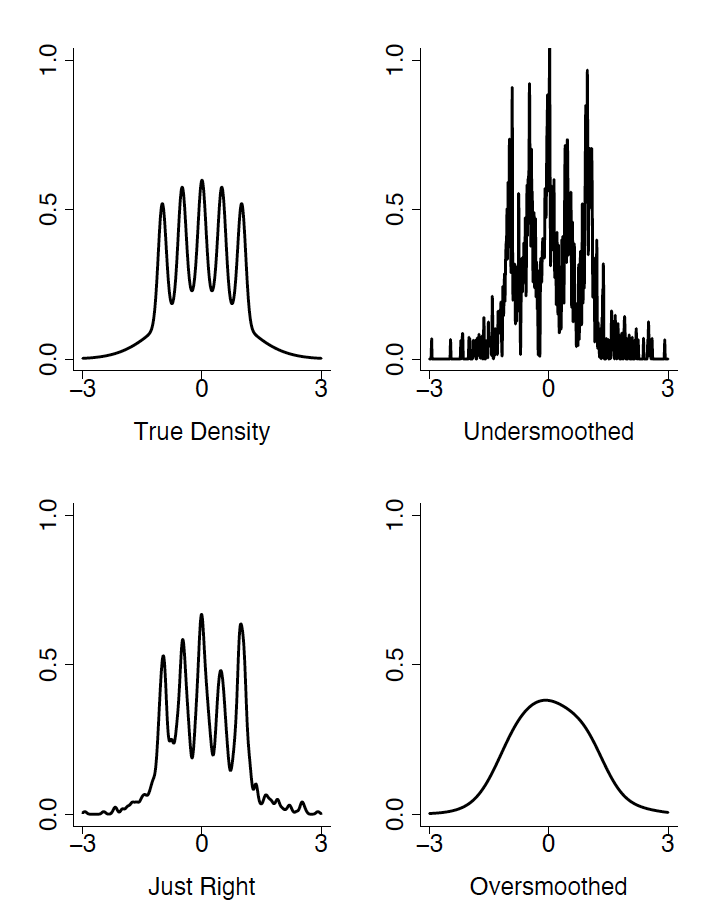
\includegraphics[width=0.5\textwidth, keepaspectratio]{smoothing.png}
\end{figure}
\end{comment}
\end{mdframed}
 \section{Curse of Dimensionality}
 Now assume that $x$ is not necessarily a scalar, but of dimension $d$. Then we can use a $d$-dimensional kernel $K$ and estimate $f(x)$ with
 \[
 \hat{f}(x)= \frac{1}{nh^d}\sum_{i=1}^nK\left(\frac{x-x_i}{h}\right)
 \]
 where $K$ can be a $d$-product of a uni-dimensional kernels. In addition, we are not necessarily confined to using a same bandwith for all $d$ kernels. For instance, if you know that the variance of $x_1$ is larger than $x_2$ you may want higher $h_1$ relative to $h_2$ to avoid variance of the kernel density estimator for the first covariate from being too large. We may want to sphericize if the kernel estimators are correlated. \par
 A bigger concern has to do with the computation cost from using a large $d$. This is what \textbf{curse of dimensionality} refers to. If we return to calculating $E[\hat{f}(x)^2]$ term in the variance component of AMISE, 
 \footnotesize{\begin{align*}
 E[\hat{f}(x)^2]&=E\left[\frac{1}{n^2h^{2d}}\left(\sum_{i=1}^nK\left(\frac{x-X_i}{h}\right)\right)^2\right]\\
 &=E\left[\frac{1}{n^2h^{2d}}\left(\sum_{i=1}^nK^2\left(\frac{x-X_i}{h}\right)+2\sum_{i<j} K\left(\frac{x-X_i}{h}\right)K\left(\frac{x-X_j}{h}\right)\right)\right]\\
 &=\frac{1}{nh^{2d}}\int_{-\infty}^\infty K^2\left(\frac{x-s}{h}\right)f(s)ds+\frac{n(n-1)}{n^2h^{2d}}\left(\int_{-\infty}^\infty K\left(\frac{x-s}{h}\right)f(s)ds\right)^2
 \end{align*}}\normalsize
 Again, the leading term is
 \[
\frac{1}{nh^{2d}}\int_{-\infty}^\infty K^2\left(\frac{x-s}{h}\right)f(s)ds \simeq \frac{1}{nh^d}\int K^2(t)f(x-ht)dt
 \]
 since $s$ is actually $d$-dimensional. Thus, the variance is now $O\left(\frac{1}{nh^d}\right)$. What this means is that $AMISE=Ah^4+\frac{B}{nh^d}$ and the optimal $h$ is solved as
 \[
 h=\left(\frac{Bd}{4An}\right)^{1/(4+d)}
 \]
 Thus, $h$ will be in $n^{-\frac{1}{4+d}}$ and convergence occurs in $n^{-\frac{2}{4+d}}$ - at an even slower rate that when $d=1$, which was already slower than parametric convergence rate. AMISE would be in order $n^{-\frac{4}{4+d}}$\par
 
 \section{Local Constant and Polynomial Estimation}
 Given the data $(y_i,x_i)$, we are attempting to capture $E[g(y,x)|x]=m(x)$ for some $g(y,x)$. For instance, we can attempt to estimate the conditional expectation by letting $g(y,x)=y$. Note that the conditional expected value can be written as
 \begin{align*}
 E[y|x]&=\int y f_{Y|X}(y|x)dy \\
 &=\int y \frac{f_{Y,X}(y,x)}{f_{X}(x)}dy=\frac{\int yf_{Y,X}(y,x)dy}{\int f_{Y,X}(y,x)dy}
 \end{align*}
 We can obtain the nonparametric estimator for the conditional expected value by replacing $f_{Y,X}$ with its kernel estimator. For simplicity, I will assume that the dimension of both $y$ and $x$ is 1. The numerator becomes
 \footnotesize{\begin{align*}
 \int y \hat{f}(y,x)dy&=\int y \frac{1}{nh^2}\sum_{i=1}^n K\left(\frac{x-X_i}{h}\right)K\left(\frac{y-Y_i}{h}\right)dy\\
 &= \frac{1}{nh^2}\sum_{i=1}^n K\left(\frac{x-X_i}{h}\right)\int yK\left(\frac{y-Y_i}{h}\right)dy\\
 &=\frac{1}{nh^2}\sum_{i=1}^n K\left(\frac{x-X_i}{h}\right)\int (Y_i+sh)K\left(s\right)(hds) \ (\because s=\frac{y-Y_i}{h})\\
 &= \frac{1}{nh}\sum_{i=1}^n K\left(\frac{x-X_i}{h}\right)Y_i\ (\because \int K(s)ds=1, \int sK(s)ds=0)
 \end{align*}}\normalsize
 The denominator can be written as $ \frac{1}{nh}\sum_{i=1}^n K\left(\frac{x-X_i}{h}\right)$. Thus, the estimator for the conditional expectation becomes
 \[
 \frac{\sum_{i=1}^n Y_iK\left(\frac{x-X_i}{h}\right)}{\sum_{i=1}^n K\left(\frac{x-X_i}{h}\right)}
 \]
 Effectively we are putting weight $\frac{K\left(\frac{x-X_i}{h}\right)}{\sum_{i=1}^nK\left(\frac{x-X_i}{h}\right)}$ on each observation $Y_i$. This is also a \textbf{local constant estimation} in the sense that when solving the following minimization problem
 \[
 \hat{f}(x)=\arg\min_a\frac{1}{nh}\sum_{i=1}^n(Y_i-a)^2K\left(\frac{x-X_i}{h}\right)
 \]
 The first order condition on $a$ yields the following results
 \[
 \sum_{i=1}^nY_iK\left(\frac{x-X_i}{h}\right)=a\sum_{i=1}^nK\left(\frac{x-X_i}{h}\right) \implies a= \frac{\sum_{i=1}^n Y_iK\left(\frac{x-X_i}{h}\right)}{\sum_{i=1}^n K\left(\frac{x-X_i}{h}\right)}
 \]
 As for the optimal $h$, it is possible to use cross-validation method and minimizing AMISE. This method can be unreliable if $f(x)\to0$. \par
 We can also do something more general. For instance, a \textbf{local linear estimation}. This is when we regress $g(y,x)$ on a constant ($a$) and a linear term ($b(x-X_i)$). In mathematical expression, we solve
 \[
 \min_{a,b}\frac{1}{nh}\sum_{i=1}^n(Y_i-a-b(x-X_i))^2K\left(\frac{x-X_i}{h}\right)
 \]
 and obtain that $\hat{a}=\hat{g}$ and $\hat{b}$ is an estimate of $\frac{\partial g(x)}{\partial x}$. If it happens that the true functional form is linear, then this estimate does not produce a bias. In addition, local linear estimation performs better than local constant estimation in the boundaries of the support for $X$. \par
 We can do even more with \textbf{local polynomial estiation} by regressing $g(y,x)$ on a constant, $x-X_i$, $(x-X_i)^2$ and so on. 
 \section{Semi-nonparametrics}
\begin{itemize}
\item Flexible approach: Suppose that we are sure that $f(x)$ can be characterized by $f_{m,\sigma}$ where $m,\sigma$ indexes some properties of the density function $f$. Then, by Weierstrass approximation theorem, we can choose a family of positive functions which increases in complexity $P_\theta^1, P_\theta^2,...$ and maximize over the loglikelihood
\[
\sum_{i=1}^n \log{f_{m,\sigma}(X_i)}P_\theta^M(X_i)
\]
\begin{mdframed}[backgroundcolor=green!5] 
\begin{theorem}[Weierstrass Approximation Theorem]  If $f$ is a continuous real-valued function on $[a,b]$ and if any $\epsilon>0$ is given, then there exists a polynomial $P$ on $[a,b]$ s.t. 
\[
|f(x)-P(x)|<\epsilon
\]
for all $x\in[a,b]$
\end{theorem}
\end{mdframed}
\item Mixture of normals: Suppose that $Y|X$ is drawn from the two distributions
\begin{itemize}
\item $N_1(m_1(x,\theta), \sigma_1^2(x,\theta))$ with probability $q_1(x,\theta)$
\item $N_2(m_2(x,\theta). \sigma_2^2(x,\theta))$ with probability $q_2(x,\theta)$
\end{itemize}
Then, we apply a maximum likelihood of the following form
\[
\min_\theta \sum_i\sum_k q_k(x_i,\theta)[(y_i-m_k(x_i,\theta))'\sigma_k(x_i,\theta)^{-1}(y_i-m_k(x_i,\theta))+\log\det{\sigma_k(x_i,\theta)}]
\]
As with other MLE estimators, there could be more than one local maxima. Furthermore, the optimal number of $k$ is difficult to determine in practice.
\item Series estimator: Let $\{P_k(x_i)|k=1,2...\}$ be the orthonormal basis for a smooth function. By orthonormal, it means that
\[
\int P_k(x)^2 dx=1, \int P_k(x) P_m(x)=0 \ (k\neq m)
\]
 These could be polynomials of degree $k$, sine functions and so on. What we do here is to run a linear regression that has the following form
\[
y_i = \sum_{k=1}^MP_k(x_i)\theta_k+\epsilon_i
\]
The $\sum_{k=1}^MP_k(x_i)\theta_k$ part is a series approximation to $g(x)$. However, depending on the number of $M$ that we choose, the curse of dimensionality can kick in. 
\end{itemize}


\section{Semiparametric Regresion}
Semiparametrics can be thought of as a middle ground between nonparametric and parametric regression. Suppose that we partition the covariates into two unoverlapping spaces - $X$ and $W$. Also assume that $E(\epsilon|X,W)=0$. One example of a semiparametric regression is a \textbf{partially linear regression} which has the following form
\[
Y_i = X_i\beta + g(W_i)+\epsilon_i 
\]
where $\beta\in\dim{(X_i)} $ represents a coefficient for the linearly regressed terms and $g(\cdot)$ is a nonparametric portion of the regression.  \par
To estimate $\beta$, we use the fact that
\begin{align*}
E[Y_i|W_i]&=E[X_i|W_i]\beta + E[g(W_i)|W_i]+E[\epsilon_i|W_i]\\
&=E[X_i|W_i]\beta + g(W_i)+E[\epsilon_i|W_i]\\
&=E[X_i|W_i]\beta + g(W_i)+E[E[\epsilon_i|X_i,W_i]|W_i] = E[X_i|W_i]\beta +g(W_i)
\end{align*}\par
Given this, we can write
\[
Y_i-E[Y_i|W_i]=\{X_i-E[X_i|W_i]\}\beta +\epsilon_i
\]\par
Then we follow this procedure
\begin{enumerate}
\item Nonparametrically estimate $E[X_i|W_i]$ and $E[Y_i|W_i]$. Then define $\tilde{X}_i=X_i-\hat{E}[X_i|W_i]$ and $\tilde{Y}_i = Y_i-\hat{E}[Y_i|W_i]$, where $\hat{E}$ are nonparametric estimators
\item Regress $\tilde{Y}$ onto $\tilde{X}$ to get an estimate of $\beta$
\item We can estimate $g(\cdot)$ by nonparametrically regressing $Y_i-X_i\hat{\beta}$ onto $W_i$
\end{enumerate}
\par
As far as approximation is concerned, $\beta$ follows the properties of parametric estimators. That is, it converges at rate $n^{-1/2}$ regardless of the dimensions of $X_i, W_i$. Thus there is no curse of dimensionality here. Unfortunately, estimating $g(\cdot)$ follows the same properties as nonparametric estimators. It has a slower convergence rate, which becomes even slower with more dimensions of $W_i$. \par
There is another caveat to this method. Identification of $\beta$ requires an exclusion restriction in the sense that none of the components in $X_i$ is perfectly predictable by $W_i$ components. If otherwise, $X_i=E[X_i|W_i]$. Thus, $\beta$ cannot be identified. This would effectively rule out including a constant in the $X_i$ part of the regression. If we do have $X_i\neq E[X_i|W_i]$, we have
\begin{gather*}
(X_i-E[X_i|W_i])'(Y_i-E[Y_i|W_i])=(X_i-E[X_i|W_i])'[(X_i-E[X_i|W_i])\beta+\epsilon_i]\\
\implies E\{(X_i-E[X_i|W_i])'(X_i-E[X_i|W_i])\}\beta=E\{(X_i-E[X_i|W_i])'(Y_i-E[Y_i|W_i])\}
\end{gather*}
The value of $\beta$ that solves the above equation is the estimator we are looking for. 
\begin{mdframed}[backgroundcolor=yellow!5] 
\begin{example}[Horowitz, Lee (2002)] The paper reviews several semiparametric methods for estimating conditional mean functions and show that semiparametrics allow more flexibility than parametric modeling and more precision than nonparametric models. For fun (at least for a baseball nerd like me), this paper tests this idea on a data of salaries, runs, tenure of baseball players in 1987. 
\end{example}
\begin{example}[Ucal et al (2010)] This paper analyzes whether and to what extent the inflow of FDI is affected before and after the occurence of a financial crisis in developing countries using generalized partial linear models. The results indicate that FDI inflows decrease in the years after a financial crisis and an upturn in FDI inflows the year before a financial crisis hit the country.
\end{example}
\end{mdframed}




\chapter{Treatment Effects: Random Assignment and Estimation under Unconfoundedness}
\section{Introduction to Treatment Effects: Causality and Treatment Assignment}
Now, our interest is in finding out whether some $X$ variable \textbf{causes} $Y$, not just whether they are correlated. Generally, correlation is not enough to argue causation. Suppose that you find that $cov(X,Y)\neq0$. This can happen because
\begin{itemize}
\item $X$ do cause $Y$, which is good for us. But..
\item $Y$ could also cause $X$. So there is a reverse causality bias here
\item $Z$ mutually affects $X$ and $Y$. This is an omitted variable bias and leads to nonzero correlation even if $X$ and $Y$ has no connection whatsoever. 
\end{itemize} \par
In any study examining program evaluation or quasi-experimental setting, the key issue is the assignment of the treatment, which is considered binary for the moment. There are three possible cases, which are
\begin{itemize}
\item \textbf{Random Assignment}: This would be a case when we can guarantee that the assignment to the treatment arms (treatment and control) are determined by chance - like flipping a coin or random draw of numbers. This rarely happens in social science, as people can voluntarily opt-in and opt-out of treatment. 
\item \textbf{Selection on Observables}: The treatment assignment is effectively random once we condition on some observable covariates. This is also known as ignorability or unconfoundedness assumptions.
\item \textbf{Selection on Unobservables}: The assignment depends fundamentally on unobservables, or in other words, we cannot break down the dependence structure of assignment using observed variables. For instance, even in a clinical trials that involve voluntary participation, it is very likely that (lack of) risk averseness determines participation. How do we control for risk averseness?
\end{itemize}
\section{Theoretical Framework for Treatment Effect}
We will consider a binary treatment variable - whether individual $i$ received a treatment or not (in the treatment group or control group). Define a variable $D_i$ s.t.

\[
D_i = \begin{cases} 1 & \text{If treated} \\ 0 & \text{If not treated}\end{cases}
\]
In the above notation, $i$ indexes the unit of the treatment - an individual, household,  county, firm, and etc. For each unit $i$, there are two possible outcomes. One is the outcome without treatment,  $Y_i(0)$. The other is the outcome with treatment, $Y_i(1)$. This can be seen as a counterfactual framework in the sense that if we get $Y_i(1)$ for unit $i$, we cannot get $Y_i(0)$ and vice versa. We always have a missing data problem in this regard. A useful way of writing this is
\[
Y_i = D_iY_i(1) + (1-D_i)Y_i(0)
\]
The left hand side is an outcome for unit $i$, treated or untreated. \textit{This is observed for every $i$}. The right hand side is meant to capture that the observed outcome for individual $i$ is either \textit{one} of $Y_i(1)$ or $Y_i(0)$. This framework is sometimes called \textbf{potential outcome framework} and will come in handy when we analyze various treatment effect results. \par
We are interested in how an outcome for unit $i$ changes between treatment and control. In other words,
\[
TE_i = Y_i(1)-Y_i(0)
\]
Another parameter of interest could be the treatment effect averaged over those who share the common covariate value, which is
\[
TE(x) = E(TE_i|X_i=x)
\]
We could also be interested in the treatment effect averaged over the population. This is the average treatment effect, defined as
\[
ATE=E(TE_i)=E(Y_i(1)-Y_i(0))
\]
Of course there are more, most of which we will learn over the course of this sequence. There are average treatment effect on the treated, ATE for the untreated, etc. \par
Because of the fundamental  problem of a missing data, we are forced to make an assumption about the things we cannot observe. Take the ATE for example. We can write
\begin{align*}
E[Y_i(1)-Y_i(0)] & = E[Y_i(1)]-E[Y_i(0)]\\
&=\{\Pr(D_i=1)E[Y_i(1)|D_i=1]+(1-\Pr(D_i=1))E[Y_i(1)|D_i=0]\}\\
&-\{\Pr(D_i=1)E[Y_i(0)|D_i=1]+(1-\Pr(D_i=1))E[Y_i(0)|D_i=0]\}
\end{align*}
Here is the problem: We can get what $E[Y_i(1)|D_i=1]$ and $E[Y_i(0)|D_i=0]$ are from the data. This is because \footnote{You might have noticed that I rarely tag equations in my recitation notes. So when I do, it means I am going back to this very often. }
\begin{gather*}
E[Y_i|D_i=1]=E[1\cdot Y_i(1)-(1-1)\cdot Y_i(0)|D_i=1]=E[Y_i(1)|D_i=1]\\
E[Y_i|D_i=0]=E[0\cdot Y_i(1)-(1-0)\cdot Y_i(0)|D_i=0]=E[Y_i(0)|D_i=0] \tag{\text{TE}}\label{TE}
\end{gather*}
So we can get $E[Y_i(1)|D_i=1]$ and $E[Y_i(0)|D_i=0]$ from the data - take the expected value of observed $Y_i$ conditional on $D_i=1 \ \text{and}\ 0$. We cannot do the same for $E[Y_i(1)|D_i=0]$ and $E[Y_i(1)|D_i=0]$. This forces us to make an assumption about what the two unobserved values could be. \par
Before going on, it would be useful to characterize the counterfactual outcome in a more econometrics-friendly context. Define the counterfactual outcomes as
\[
Y_i(D_i=d)=\mu(X_i,d)+\epsilon_i(d)
\]
where $d$ can take either $0, 1$. What we want to learn involves understanding the joint distribution of the variables $Y_i(0)$ and $Y_i(1)$. Take the treatment effect at $X_i=x$, written as
\[
TE(x)=\mu(x,1)-\mu(x.0)
\]
This is the effect of the treatment on the outcome $Y_i$ for $X_i=x$. The interpretation is that if we shift everyone with $X_i=x$ from the control group to the treatment group, the average outcome increases by $TE(x)$. We can also calculate ATE as
\begin{align*}
ATE&=E[Y_i(1)-Y_i(0)]=E[\mu(X_i,1)-\mu(X_i,0)+\epsilon_i(1)-\epsilon_i(0)]\\
&=E\left[E[\mu(X_i,1)-\mu(X_i,0)+\epsilon_i(1)-\epsilon_i(0)|X_i]\right]=E\left[E[\mu(X_i,1)-\mu(X_i,0)|X_i]\right]\\
&=E[\mu(X_i,1)-\mu(X_i,0)]=E[TE(X_i)]
\end{align*}
\section{Randomized Assignment}
We are back to having to assume what $E[Y_i(1)|D_i=0]$ and $E[Y_i(1)|D_i=0]$ are. A \textbf{random assignment} assumes that the outcome is independent of the treatment status. More formally
\[
(Y_i(0), Y_i(1))\perp \!\!\! \perp D_i \ \tag{\text{RA}}\label{RA}
\]
This implies that
\[
E[Y_i(1)]=E[Y_i(1)|D_i=1]=E[Y_i(1)|D_i=0]
\]
and similarly for $E[Y_i(0)]$. If we go back to the (\ref{TE}) equation, the problem was that we were unable to make any statement about $E[Y_i(1)|D_i=0]$ and $E[Y_i(1)|D_i=0]$. Now what we are doing is to equate
\begin{gather*}
E[Y_i|D_i=1]=E[Y_i(1)|D_i=1]=E[Y_i(1)|D_i=0]\\
 E[Y_i|D_i=0]=E[Y_i(0)|D_i=0]=E[Y_i(0)|D_i=1]
\end{gather*}
and effectively make the statements about the previously unobserved values. This allows us to rewrite the ATE as 
\begin{align*}
E[Y_i(1)-Y_i(0)]&=E[Y_i(1)]-E[Y_i(0)]\\
&=E[Y_i(1)|D_i=1]-E[Y_i(0)|D_i=0] \ (\because \ref{RA})\\
&=E[Y_i|D_i=1]-E[Y_i|D_i=0] \ (\because \ref{TE})
\end{align*}
Therefore, we can estimate ATE by mapping $E[Y_i(1)]$ to $E[Y_i|D_i=1]$, $E[Y_i(0)]$ to $E[Y_i|D_i=0]$. 
\section{Conditional Independence Assumption}
In this setup, we are assuming that conditional on $X_i$, the outcomes and $D_i$ are independent. Formally, we can write
\[
 (Y_i(0), Y_i(1)) \perp \!\!\! \perp D_i|X_i \ \tag{\text{CIA}}\label{CIA}
\]
We can alternatively conceptualize this framework in the following way: Define $D_i$ as
\[
D_i = 1(u_i<p(X_i))
\]
where $u_i\equiv U[0,1]$ determines selection and $p(X_i)$ can be interpreted as a propensity score - how much are you likely to be treated given that you have covariates specified as some $X_i$. This framework, along with the (\ref{CIA}), allows us to say the following:
\footnotesize{\begin{align*}
E[Y_i(1)|X_i=x]&=E[Y_i(1)|D_i=1,X_i=x]=E[Y_i(1)|D_i=0,X_i=x] \ (\because \ref{CIA})\\
&\implies E[\mu(x,1)+\epsilon_i(1)|D_i=1,X_i=x]=E[\mu(x,1)+\epsilon_i(1)|D_i=0,X_i=x]\\
&\implies E[\mu(x,1)|D_i=1,X_i=x]-E[\epsilon_i(1)|D_i=1,X_i=x]\\
&=E[\mu(x,1)|D_i=0,X_i=x]+E[\epsilon_i(1)|D_i=0,X_i=x]\\
&\implies E[\epsilon_i(1)|D_i=1,X_i=x]=E[\epsilon_i(1)|D_i=0,X_i=x]\ (\because \mu(x,1)\text{ is same for both cases})\\
&\implies E[\epsilon_i(1)|u_i<p(x),X_i=x]=E[\epsilon_i(1)|u_i>p(x),X_i=x]\\
&\implies (\epsilon_i(1), \epsilon_i(0))\perp \!\!\! \perp u_i|X_i \tag{\text{CIA2}}\label{CIA2}
\end{align*}}\normalsize
Thus, conditional on observed values for the covariate $X_i$, the unobserved elements of the selection rule $u_i$ are independent of the unobserved elements of the error process $(\epsilon_i(1), \epsilon_i(0))$.\par
 The caveat, however, is that $p(x)\in(0,1)$. If $p(x)=1$, then for every possible $u_i$, $D_i=1$ - everyone gets treated. Therefore, there is no meaningful statement we can make about the $D_i=0$ case. We can say similarly for $p(x)=0$ case. In some textbooks, this is also known as \textbf{overlap} assumption - each unit in the defined population should have some chance of being treated and some chance of being in the control group. \footnote{If both (\ref{CIA}) and overlap is satisfied, we say that have \textbf{strong ignorability} (Rosenbaum, Rubin 1983).} \par
Under CIA, we can derive the treatment effect as follows
\footnotesize{\begin{align*}
E[Y_i|D_i=1, X_i=x]-E[Y_i|D_i=0, X_i=x]&=E[\mu(x,1)+\epsilon_i(1)|D_i=1, X_i=x]-E[\mu(x,0)+\epsilon_i(0)|D_i=0, X_i=x]\\
&=E[\mu(x,1)|D_i=1, X_i=x]+E[\epsilon_i(1)|D_i=1, X_i=x]\\
&-E[\mu(x,0)|D_i=0, X_i=x]-E[\epsilon_i(0)|D_i=0, X_i=x]\\
&=\mu(x,1)+E[\epsilon_i(1)|X_i=x]-\mu(x,0)-E[\epsilon_i(0)|X_i=x] \ (\because \ref{CIA2})\\
&=\mu(x,1)-\mu(x,0)
\end{align*}}\normalsize
Note that 
\footnotesize{\begin{align*}
E[Y_i(1)-Y_i(0)|X_i=x] &= E[Y_i(1)|X_i=x]- E[Y_i(0)|X_i=x]\\
&=(\Pr(D=1|X_i=x)\cdot E[Y_i(1)|D_i=1,X_i=x]+(1-\Pr(D=1|X_i=x))E[Y_i(1)|D_i=0,X_i=x])\\
&-(\Pr(D=1|X_i=x)\cdot E[Y_i(0)|D_i=1,X_i=x]+(1-\Pr(D=1|X_i=x))E[Y_i(0)|D_i=0,X_i=x])\\
&=  E[Y_i(1)|D_i=1,X_i=x]- E[Y_i(0)|D_i=0,X_i=x] \ (\because \ref{CIA}) \\
&=  E[Y_i|D_i=1, X_i=x]-E[Y_i|D_i=0, X_i=x]
\end{align*}}\normalsize
Thus, under (\ref{CIA}) we can back out the ATE for $X_i=x$ using the observables. This assumption allows us to map $ E[Y_i(1)|X_i=x]$ to $ E[Y_i|D_i=1, X_i=x]$ and $E[Y_i(0)|X_i=x]$ to $ E[Y_i|D_i=0, X_i=x]$, which is impossible without it. \par
This is called a \textbf{regression adjustment} method. The treatment effect for $X_i=x$ using a regression adjustment can be obtained by utilizing the fact that 
\[
\mu(x,1)=E[Y_i|D_i=1, X_i=x], \ \mu(x,0)=E[Y_i|D_i=0, X_i=x]
\]
and regressing on the subsample of each treatment arm to get $\hat{\mu}(x,1)$ and $\hat{\mu}(x,0)$. Thus
\[
\frac{1}{N}\sum_{i=1}^N(\hat{\mu}(x,1)-\hat{\mu}(x,0))
\]
\section{Inverse Probability Weighting}
We can obtain the average treatment effect using a different approach. This is an \textbf{inverse probability weighting}. The steps are as follows
\begin{enumerate}
\item Estimate the propensity score $p(X_i)$ by computing
\[
\hat{p}_n(X_i)=\Pr(D_i=1|X_i=x)
\]
\item Use the magic formula to estimate $E(TE(x)|x\in A)$: That is,
\[
\frac{\sum_{D_i=1,x_i\in A}a_iY_i}{\sum_{D_i=1,x_i\in A}a_i}- \frac{\sum_{D_i=0,x_i\in A}b_iY_i}{\sum_{D_i=0,x_i\in A}b_i}
\]
where $a_i=\frac{1}{\hat{p}_n(x_i)}, b_i=\frac{1}{1-\hat{p}_n(x_i)}$. The above can also be written as
\[
\frac{\sum_{i=1,x_i\in A}^N\frac{D_iY_i}{\hat{p}(X_i)}}{\sum_{i=1,x_i\in A}^N\frac{D_i}{\hat{p}(X_i)}}-\frac{\sum_{i=1,x_i\in A}^N\frac{(1-D_i)Y_i}{1-\hat{p}(X_i)}}{\sum_{i=1,x_i\in A}^N\frac{1-D_i}{1-\hat{p}(X_i)}}\]
\end{enumerate}\par
The reason this works is as follows: Notice that
\begin{align*}
D_iY_i& = D_i(D_iY_i(1)+(1-D_i)Y_i(0))=D_iY_i(1)\\
(1-D_i)Y_i&=(1-D_i)Y_i(0)
\end{align*}
Thus, we have
\begin{align*}
E\left[\frac{D_iY_i}{p(X_i)}\right]&=E\left[E\left[\frac{D_iY_i(1)}{p(X_i)}|X_i\right]\right]\\
&=E\left[\frac{E[D_i|X_i]E[Y_i(1)|X_i]}{p(X_i)}\right]\\
&=E\left[\frac{p(X_i)E[Y_i(1)|X_i]}{p(X_i)}\right]=E[E[Y_i(1)|X_i]]=E[Y_i(1)]
\end{align*}
so we have $E\left[\frac{D_iY_i}{p(X_i)}\right]=E[Y_i(1)], E\left[\frac{D_iY_i}{p(X_i)}|X_i\right]=E[Y_i(1)|X_i]$. We can make the similar arguments for $Y_i(0)$ and get $E\left[\frac{(1-D_i)Y_i}{1-p(X_i)}\right]=E[Y_i(0)], E\left[\frac{(1-D_i)Y_i}{1-p(X_i)}|X_i\right]=E[Y_i(0)|X_i]$. Thus, the ATE for $X_i\in A$ can be written as
\[
\frac{1}{N}\sum_{i=1}^N\left(\frac{D_i Y_i}{p(X_i)}-\frac{(1-D_i)Y_i}{1-p(X_i)}\right) \ \forall X_i\in A
\]
In most cases, the propensity score is estimated. So we use the estimator involving the $\hat{p}$, which is what we have in the lecture notes. It is said that normalizing the weights to one in finite samples improves the mean squared error properties of the estimator (Imbens, Rubin (2019) - \textit{Causal Inference for Statistics, Social, and Biomedical Sciences: An Introduction})
\section{Matching Estimation}
The idea behind matching estimation is to impute the values for something we cannot get from the data: Namely,  $Y_i(0)$ for those in $D_i=1$ and $Y_i(1)$ for those in $D_i=0$. In other words, you try to find a `close' match for a particular unit $i$ in a different treatment arm. When we say we find $k$-closest neighbors for unit $i$ in $D_i=0$, we find $k$ individuals in $D_i=1$ that has close traits ($X_i$) to individual $i$, or $k$ individuals with the smallest values of $||x_j - x_i||$. Then, we construct a counterfactual $Y_i(1)$ by taking a (weighted) average over the $Y_i$'s of the $k$ individuals found in the other group. The treatment effect would than be $Y_i(1)$ -$Y_i$, where $Y_i(1)$ is calculated as in previous sentence. \par
Let's try with $k=1$ - we find the one individual in the opposite treatment arm that has the similar value of $X_i$. Then, the average treatment effect can be written as
\[
\frac{1}{N}\sum_{i=1}^N(\hat{Y}_i(1)-\hat{Y}_i(0))
\]
where
\[
\hat{Y}_i(1)=\begin{cases} Y_i & (D_i=1) \\ \text{imputed value} & (D_i=0)\end{cases}, \ \hat{Y}_i(0)=\begin{cases} \text{imputed value} & (D_i=1) \\ Y_i & (D_i=0)\end{cases}
\]
\par
There are some caveat in this approach
\begin{itemize}
\item The covariate $X_i$ that is used to find the closest match in the other treatment arm should not affect the assignment of the treatment. In other words, if the assignment of treatment vs. control depends on some subset of $X_i$, you should not use that subset as a standard for finding the closest match.
\item The overlap condition becomes critical. If it is not satisfied, i.e. for some $X_i$, $p(X_i)=1$ or $0$, then we are unable to find a closest match in the other treatment arm because for individuals with that covariate value, all of them are either in control or treatment group and not spread around. 
\item Who are the neighbors? The answer might depend on what distance measure we use. Moreover, how many of those in the treatment can be considered neighbors? There is a trade-off in the sense that using larger $k$ would force us to put someone who is not `close' as neighbors and using small $k$ may cause difficulty in imputing counterfactual values. 
\end{itemize}

\section{Difference-in-Difference Estimation}
This involves a specific framework where we can clearly define a `before and after' - denoted as $t_0$ and $t_1$. No one is treated at $t_0$ but there is a subset of people ($G_i=1$) that are treated at $t_1$. Those in $G_i=0$ are never treated in either time period. If we define
\[
Y_{i,t}=G_iY_{i}(1,t)+(1-G_i)Y_{i}(0,t) \ \ (t\in\{t_0, t_1\})
\]
and impose
\[
Y_i(G_i, t_0)=Y_{i}(t_0) \ \ \text{for both }G_i=1 \ \text{and }G_i=0 
\]
then we will be able to observe $(Y_{i,t_1}, Y_{i,t_0},G_i. X_i)$ for every unit $i$. What we do not observe is $Y_i(1,t_1)$ for those in $G_i=0$ and $Y_i(0,t_1)$ for those in $G_i=1$.  The analogue to the conditional independence assumption in this context is a \textbf{parallel trend assumption}, defined as
\[
(Y_i(1,t_1)-Y_i(t_0), Y_i(0,t_1)-Y_i(t_0)) \perp\!\!\! \perp G_i|X_i
\]\par
To see why they are equal, consider a setting where $D_i=G_i$ and write
\begin{align*}
Y_i = Y_{i,t_1}-Y_{i,t_0}&=D_i(\underbrace{Y_i(1,t_0)-Y_i(1,t_0)}_{Y_i(1)})+(1-D_i)(\underbrace{Y_i(0,t_1)-Y_i(0,t_0)}_{Y_i(0)})\\
&=D_iY_i(1) + (1-D_i)Y_i(0)
\end{align*}
Therefore, we can rewrite the parallel trend assumption as
\[
(Y_i(1), Y_i(0)) \perp\!\!\! \perp D_i|X_i
\]
which is the same as the conditional independence assumption. \par
To apply this in regression, we can write
\[
Y_{it}=\beta_0(X_i)+\beta_1(X_i)\cdot1(t=t_1)+\beta_2(X_i)\cdot G_i + \beta_3(X_i)\cdot G_i\cdot1(t=t_1)+\epsilon_{it}
\]
where $X_i$ is a set of covariates, which can include a constant. In this context, the treatment effect for $X_i=x$ would be
\begin{align*}
TE(x)&=E[Y_i(1)-Y_i(0)|X_i=x]\\
&=E[(Y_i(1,t_1)-Y_i(1,t_0))-(Y_i(0,t_1)-Y_i(0,t_0))|X_i=x]\\
&=x\cdot E\{[(\beta_0+\beta_1+\beta_2+\beta_3)-(\beta_0+\beta_2)]-[(\beta_0+\beta_1)-(\beta_0)]|X_i=x\}\\
&=x\cdot E[(\beta_1+\beta_3)-\beta_1|X_i=x]\\
&=\beta_3 x
\end{align*}
So $\beta_3$ would be our parameter of interest. \par
One difficulty arises from testing the parallel trends assumption. Loosely speaking, what we can do is to select a time period $\tilde{t}<t_0$ and find out if the difference $y_i(t_0)-y_i(\tilde{t})$ is independent with $G_i$. If not independent, we say that there is an autonomous trend. 

%%%%%%%%%%%%%%%



\chapter{Treatment Effects: Selection on Unobservables}
\section{Violation of Conditional Independence Assumptions}
There are cases where the assignment, even if we condition on observables, are not random. So in the regressional framework of $y_{i}(d)=\mu(X_i,d)+\epsilon_i(d)$, the error terms is not independent of $D_i|X_i$. The conditional independence assumption can be broken because:
\begin{itemize}
\item Participants self-select based on expected benefit: Think about a job training program for plumbing. Then, maybe those who are more healthy and suffer less in terms of costs are likely to join. If health is not perfectly observed, we risk breaking the conditional independence assumption
\item Participants may be selected, consciously or not, to join: Think of the clinical trial where participation is voluntary. In such case, individuals who are more risk-loving are more likely to join. In other words, participants and nonparticipants systematically differ on risk-averseness - something that is not usually observed.
\item There may be equilibrium effects: A tuition subsidy program that intends to increase the number of people entering college may have a spillover effect by increasing supply of college graduates at the labor market, leading to a decrease in college premium. This may induce students to enter college less. If TE is the (rate of) college entrance, such equilibrium effect may be influential.  
\end{itemize}
\par
Mathematically, what happens is that when we calculate $E[Y_i|D_i=1,x]-E[Y_i|D_i=0,x]$, we end up with
\begin{align*}
E[Y_i|D_i=1,x]-E[Y_i|D_i=0.x]&=\mu(x.1)-\mu(x,0)+E[\epsilon_i(1)|D_i=1,x]-E[\epsilon_i(0)|D_i=0,x]\\
&=TE+E[\epsilon_i(1)|D_i=1,x]-E[\epsilon_i(0)|D_i=0,x]
\end{align*}
The error term no longer can be erased from the equation since CIA assumption is not applicable. The difference between the error term is the \textbf{selection bias} (Also appears in Angrist, Pischke 2009). This also means that the error terms and the $u_i$ in $D_i=1(u_i<p(x_i))$ can covary. The result is that the treatment effect estimated from here can be inaccurate. \par
There are two possible solutions. Old method relies on \textbf{Heckman correction}. Recent focus is on IV to derive \textbf{marginal treatment effects} and \textbf{localized average treatment effect}.
\section{A Brief Discussion of the Heckman Correction}
Suppose that we are in the situation where we have a data generating process
\[
Y_i = \max\{X_i\beta+\sigma\eta_i, 0\}, \eta_i \sim N(0,1)
\]
So we only see $Y_i$ if $X_i\beta+\sigma\eta_i>0$. We are able to observe $D_i$, specified as
\[
D_i=\begin{cases}1 & \text{if }\eta>-\frac{X_i\beta}{\sigma}\\ 0 & \text{otherwise} \end{cases}
\]
Then, for the observed sample, we are likely to have an $\eta_i$ that is positively selected. So the idiosyncratic error is no longer random and we have a biased estimates, shown as (assuming $X_i$ is observable)
\footnotesize{\begin{align*}
E[Y_i|Y_i>0]&= X_i\beta + E[\sigma\eta_i|Y_i>0]\\
\implies E[\eta_i|Y_i>0]& =E\left[\eta_i| \eta_i>-\frac{X_i\beta}{\sigma}\right]=\int_{-X_i\beta/\sigma}^\infty t\phi(t|\eta_i>-X_i\beta/\sigma)dt\\
&=\int_{-X_i\beta/\sigma}^\infty t\frac{\phi(t)}{\Pr(\eta_i>-X_i\beta/\sigma)}dt =\frac{1}{1-\Phi(-X_i\beta/\sigma)}\int_{-X_i\beta/\sigma}^\infty t\frac{1}{\sqrt{2\pi}}e^{-t^2/2}dt\\
&=\frac{1}{1-\Phi(-X_i\beta/\sigma)}\left[\frac{1}{\sqrt{2\pi}}e^{-t^2/2}\right]_{-X_i\beta/\sigma}^\infty=\frac{\phi(-X_i\beta/\sigma)}{1-\Phi(-X_i\beta/\sigma)}\\
&=\frac{\phi(X_i\beta/\sigma)}{\Phi(X_i\beta/\sigma)}=m(-X_i\beta/\sigma)\neq0\\
\end{align*}}\normalsize
So the error has nonzero conditional mean. The ratio of the pdf over cdf $\frac{\phi(\cdot)}{\Phi(\cdot)}$ is the inverse Mill's ratio (IMR). Heckman's correction uses the IMR to correct for the bias. The challenge is to identify $\beta/\sigma$. We do this by
\begin{enumerate}
\item Use probit to regress $D_i$ onto $X_i$. Then we can obtain $\widehat{\beta/\sigma}$.
\item Define $\hat{f}(x)=m(-X_i\widehat{\beta/\sigma})$. We include $\hat{f}(x)$ in the control variable and run
\[
Y_i = X_i\beta+ \gamma\hat{f}(x)+\epsilon_i
\]
on the participant sample. 
\end{enumerate}\par
The problem is that we assume the normality of the error term and the linearity of the DGP, which is not always true. Thus, it is not always an ideal way to deal with selection on unobservables. 
\section{Instrumental Variables}
In this setup, you assume that there exist variables $Z_i$ that affect the treatment $D_i$ but not the outcomes (at least on its own). It should satisfy
\begin{itemize}
\item \textbf{Relevancy}: It effects the propensity score $p(x,z)=\Pr(D_i=1|X_i=x, Z_i=z)$
\item \textbf{Validity}: Distribution of the counterfactual outcomes and $u_i$ does not depend on $Z_i|X_i$. To put it in mathematical notation, 
\[
(Y_i(1), Y_i(0), u_i) \perp \!\!\!\perp Z_i|X_i
\]
\begin{mdframed}[backgroundcolor=yellow!5] 
\begin{comment}[Some remarks about the above condition] Note that $u_i$ is tied together with the potential outcomes. This implies that $u_i$ and the outcome can be correlated, which is allowed in a non-CIA setup. What matters is that the changes in $Z_i$ not affect $u_i$
\end{comment}
\begin{comment}[Violation of validity]  Let $Z_i$ change from $z$ to $z'>z$ and that the propensity rises with $z$. Suppose that for a fixed $X_i=x$, $p(x,z)>u_i$. So $D_i=1$ in this case. If we have $p(x,z')<u_i'$, then $D_i=0$. In addition, we may have the change of $z$ itself affecting the outcome directly with the violation of the validity condition.  
\end{comment}
\begin{comment}[So who are we identifying?] If $u$ is independent of $Z_i$ given $X_i$, then by moving from $p(x,z)$ to some $p(x,z')$, we can find a group of individuals who do not get treated at $p(x,z)$ but do get treated at $p(x,z')$. We refer to them as \textbf{compliers}. If people were participating at $p(x,z)$ they participate at $p(x,z')$. We then have a group of \textbf{always takers}. Conversely, if people do not get treated at $p(x,z')$, they don't get treated at lower propensity scores - the \textbf{never takers}. \par
We do not identify \textbf{defiers} - they have $u_i<p(x,z)$ but $u_i'>p(x,z')>p(x,z)$. The only way this can happen is if $u_i$ changes with $z_i$ - a violation of validity. This is sometimes called as monotonicity condition or no two-way movement condition. 

\end{comment}
\end{mdframed}
\item \textbf{Full support}: The support of $p(x,z)$ conditional on $x$ extends to all of $[0,1]$. This implies that change in $Z$ induces large variations in the propensity score. 
\end{itemize} 
\par
So what concerns do we run into in terms of identification? We can identify $p(x,z)$ by calculating $\Pr(D_i=1|X_i=x, Z_i=z)$. We can also write
\begin{align*}
E[Y_i|D_i=1, X_i=x, Z_i=z]&=\mu(x,1)+E[\epsilon_i(1)|u_i<p(x,z), X_i=x, Z_i=z]\\
&=\mu(x,1)+E[\epsilon_i(1)|u_i<p(x,z), X_i=x] \ (\because\text{validity})
\end{align*}
Define $K_1(p(x,z))=E[\epsilon_i(1)|u_i<p(x,z), X_i=x]$ to be some unknown function of the conditional expectation of $\epsilon_i(1)$. We can also work similarly to define 
\[
E[Y_i|D_i=0, X_i=x, Z_i=z]=\mu(x,0)+E[\epsilon_i(0)|u_i>p(x,z), X_i=x]
\] 
and $K_0(p(x,z))=E[\epsilon_i(0)|u_i>p(x,z), X_i=x]$. Note that the left hand sides for both sets of equations can be identified by naively taking an average of $Y_i$'s conditional on some the treated (untreated) for the group $X_i=x, Z_i=z$. The estimated result breaks down into
\[
\mu(x,1)-\mu(x,0)+\underbrace{K_1(p(x,z))-K_0(p(x,z)) }_{\Delta(p(x,z))}= TE(x)+\Delta(p(x,z))
\]
The $\Delta(p(x,z))$ is the control function that stands for the selection bias. By the relevance condition, the change in $z$ affects the value of $p(x,z)$ for a fixed $x$. So changing $z$ allows us to identify how $\Delta(p(x,z))$ \textit{changes}. However, we do not know what the \textit{exact value} of $\Delta(p(x,z))$ is for the initial value of $z$ we started. Therefore, the true parameter of interest, which is TE, cannot be uncovered. \par
So how can we progress on? Note that the $K_d$ functions are conditional expectations of $\epsilon_i(d)$ on $X_i=x$ and selection rule $u_i (<,>) p(x,z)$. In particular, we can get that
\begin{align*}
K_1(1) &=E[\epsilon_i(1)|u_i<1,X_i=x] \\
&=E[\epsilon_i(1)|X_i=x] \ (\because\text{Everyone is treated})\\
&=0\\
K_0(0) &=E[\epsilon_i(1)|u_i>0,X_i=x] \\
&=E[\epsilon_i(1)|X_i=x] \ (\because\text{No one is treated})\\
&=0
\end{align*}
Heckman and Vytlacil show that if we are given a continuous instrument $z$, we can do a much better job of identifying the treatment effect. 
\section{Marginal Treatment Effects}
The \textbf{marginal treatment effect} at $p(x,z)=p$ is defined as the treatment effect on individuals whose $u_i=p(x,z)$. We can write
\[
MTE(p)=E[Y_i(1)-Y_i(0)| u_i=p]
\]
The conditional expectation above is not directly obtainable from the data. Heckman and Vytlacil show that 
\[
MTE(p)=\frac{\partial E[Y_i | p(x,z)=p]}{\partial p}
\]
which is obtainable from the data. This is done by 
\begin{enumerate}
\item Estimate $p(x,z)=\Pr(D_i=1|X_i=x. Z_i=z)$
\item Regress $Y_i$ on the estimated $p(x,z)$ in a flexible setting - preferably not just linearly but with some nonlinearities
\item Take a derivative with respect to $p$. (or local linear estimator)
\item For treatment effects, evaluate the $E[Y_i|p(x,z),x]$ at $p(x,z)=1$ and $p(x,z)=0$ and identify the difference. (You can obtain $E[Y_i|\cdot]$ by getting the predicted values).  
\end{enumerate}
\par
Intuitively, what is going on with MTE is as follows: By changing $p$ slightly by $dp$, we are able to identify the marginal compliers who move from not being treated to being treated. We are finding out how their outcome changes as they move from non-participation to participation into the treatment. \par
To see why the above result holds, we define
\[
G(p)=E[Y_i\cdot 1(p(x,z)=p)]
\]
Since $Y_i=D_iY_i(1)+(1-D_i)Y_i(0)=1(u_i<p(x,z))Y_i(1)+1(u_i>p(x,z))Y_i(0)$, we can rewrite the above as
\begin{align*}
G(p)&=E[Y_i(1)\cdot 1(u_i<p(x,z))\cdot 1(p(x,z)=p)+Y_i(0)\cdot 1(u_i>p(x,z))\cdot 1(p(x,z)=p)]\\
&=E[Y_i(1)\cdot 1(u_i<p)\cdot 1(p(x,z)=p)]+E[Y_i(0)\cdot 1(u_i>p)\cdot 1(p(x,z)=p)]\\
&=G_1(p)+G_0(p)
\end{align*}
By the validity condition and the fact that $u_i\sim U[0,1]$ (and thus $f(u_i)=1$), we can write
\begin{align*}
E[Y_i(1)\cdot 1(u_i<p)\cdot 1(p(x,z)=p)]&=E[Y_i(1)\cdot 1(u_i<p)]\Pr(p(x,z)=p)\\
&=\int_0^pE[Y_i(1)|u=t]dt\Pr(p(x,z)=p)
\end{align*}
And similarly, 
\[
E[Y_i(0)\cdot 1(u_i>p)\cdot 1(p(x,z)=p)]=\int_p^1E[Y_i(0)|u=t]dt\Pr(p(x,z)=p)
\]
So 
\footnotesize{\[
E[Y_i\cdot 1(p(x,z)=p)]=G(p)=\left(\int_0^pE[Y_i(1)|u=t]dt+\int_p^1E[Y_i(0)|u=t]dt\right)\Pr(p(x,z)=p)
\]}\normalsize
with the fact that $E[Y_i\cdot 1(p(x,z)=p)]=E[Y_i|p(x,z)=p]\cdot \Pr(p(x,z)=p) $ this implies that
\footnotesize{\[
E[Y_i|p(x,z)=p]=\frac{G(p)}{\Pr(p(x,z)=p)}=\int_0^pE[Y_i(1)|u=t]dt+\int_p^1E[Y_i(0)|u=t]dt
\]}\normalsize
Then, by Leibniz's integral rule
\[
\frac{\partial E[Y_i | p(x,z)=p]}{\partial p}=E[Y_i(1)|u=p]-E[Y_i(0)|u=p]=MTE(p)
\]
Hence, the treatment effect can be recovered by
\[
TE=\int_0^1MTE(p)dp=E[Y_i|p(x,z)=1]-E[Y_i|p(x,z)=0]
\]

\section{Some Large Caveats for MTE}
For the above methods to work, we need the $Z_i$ instruments to satisfy
\begin{itemize}
\item $Z$ belongs in the treatment equation (relevancy): $D_i=1(u_i<p(X_i,Z_i))$
\item $Z$ does not belong in the outcome equation (exclusivity): $Y_i(d)=\mu(x,d)+\epsilon_i(d)$
\item In other words, we get $(\epsilon_i(1), \epsilon_i(0), u_i) \perp\!\!\!\perp Z_i|X_i$
\item Continuity: $p(x,z)$ changes w.r.t $z$ in a continuous way (This is because we need to be able to take derivatives)
\end{itemize}
For the range of $p(x,z)$ available, the above condition allows us to estimate the marginal treatment effect. For any work you see that uses marginal treatment effect, there includes a graph that maps marginal treatment effect on the vertical axis and the `resistance' parameter $u_i$ on the horizontal axis. \par
With this framework, we can also test if conditional independence assumption holds. Recall that conditional independence assumption is satisfied when
\[
(\epsilon_i(1),\epsilon_i(0)) \perp\!\!\!\perp u_i|X_i
\]
In cases where this is true, then the outcomes are independent of $u_i$ conditional on $X_i$. Thus, 
\[
MTE(x,p)=E[Y_i(1)-Y_i(0)|X_i=x, u_i=p]=E[Y_i(1)-Y_i(0)|X_i=x]
\]
Since $MTE(x,p)=\frac{\partial E[Y_i | X_i=x, p(x, z)=p]}{\partial p}$, the above condition implies that $E[Y_i|X_i=x, p(x, z)=p]$ is linear in $p$. Thus, it is highly recommended to put polynomial terms of $p^k, k=1,2,3,...$ when you estimate marginal treatment effects. Then, test to find whether the nonlinear terms have coefficient zero. 
\par 
So what do we gain by testing the form of $MTE(x,p)$? How it varies with $p$ may inform how well the treatment is designed. Ideally, we want the treatment to be applied to those who are more likely to be benefitted by it. If $p$ is higher for those with larger benefits, then the design is well-targeted.
\begin{mdframed}[backgroundcolor=blue!5] 
\begin{definition}[Policy Relevant Treatment Effect]  Policy relevant treatment effect is the mean effect of going from a baseline policy to a new policy per net person shifted (Heckman, Vytlacil 2001, Carneiro, Heckman, Vytlacil 2010). This can be written as
\begin{gather*}
\frac{E[Y_i|\text{New Policy}]-E[Y_i|\text{Old Policy}]}{E[D_i|\text{New Policy}]-E[D_i|\text{Old Policy}]}\\
=\int_0^1MTE(u)\omega(x,u) du\  \  \ \ (\omega(x,u)=F_{P_{old}|X}(u|x)-F_{P_{new}|X}(u|x))
\end{gather*}
\end{definition}
\end{mdframed}

\begin{mdframed}[backgroundcolor=yellow!5] 
\begin{example}[Carneiro \& Lee, 2019] The paper estimates the impact of attending college on log wage distributions. The paper finds that individuals more likely to attend college (and have low resistance parameters) are more likely to have higher college wage ($Y_i(1)$) over high school wage ($Y_i(0)$). The opposite holds true for people with high school degree. They have a MTE figure (at figure 3) that maps MTE as a function of resistance parameters.
\end{example}
\begin{example}[Johnson \& Taylor, 2019] The paper shows that causal impact of migration decreases longevity. This is even with the consideration that migrants are more likely to be educated and have higher baseline earnings compared to non-migrants. They use the MTE to (with railcar traffic at the town of origin as one of their IVs). They document that those who have lower latent ability (high $U_d$) suffer more from migrating out, reflected in the downward sloping MTE 
\end{example}
\centering
\begin{figure}[H]
\begin{subfigure}{0.5\textwidth}
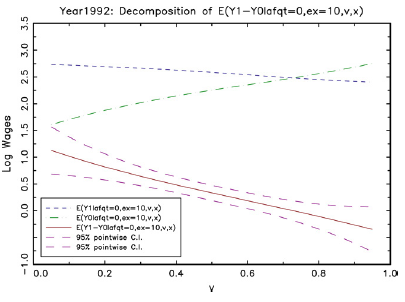
\includegraphics[width=\textwidth]{fig11_1}
\caption{Carneiro, Lee (2009)}
\end{subfigure}
\begin{subfigure}{0.5\textwidth}
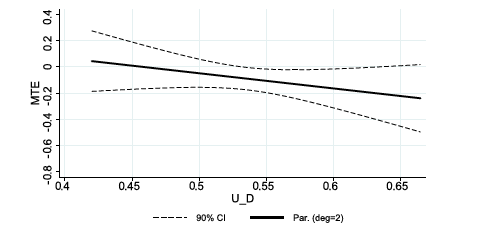
\includegraphics[width=\textwidth]{fig11_2}
\caption{Johnson, Taylor (2019)}
\end{subfigure}
\end{figure}
\end{mdframed}
\section{Local Average Treatment Effect}
The marginal treatment effect looks at `marginal' compliers: It is interested in the small group of individuals who changes treatment status from $D_i=0$  to $D_i=1$ as $p(x,z)$ changes slightly due to $Z_i$. Instead of changing the propensity score by a tiny bit (thanks to the continuity of the instrument $Z_i$), we can look at finite differences - like $Z_i$ having just two possible values. Then we are going to be looking at a larger group of compliers than in the marginal treatment effect context. The treatment effect for this larger group of compliers is called \textbf{local average treatment effect}. \par
We will setup the framework as follows:
\begin{itemize}
\item $Z_i$ will be a binary instrumental variable. This of this as an eligibility rule. 
\item $D_i(z)$ can be characterized as $D_i(z)=1(u_i<p(x,z))$. Note that as $z$ rises, so will $p(x,z)$. This is the relevance condition
\item $Z_i$ itself has no bearing, at least directly, on the outcome. So $Y_i(d)=\mu(x,d)+\epsilon_i(d)$. So we still have $(\epsilon_i(1), \epsilon_i(0), u_i)\perp\!\!\!\perp Z_i|X_i$. 
\end{itemize}
The formal way to define local average treatment effect is as follows
\[
LATE(x)=E[Y_i(1)-Y_i(0)|p(x,z)<u_i<p(x,z'). X_i=x]
\]
We can identify LATE by using the following (I skip $X_i=x$)
\footnotesize{\begin{align*}
E[Y_i|Z_i=z']-E[Y_i|Z_i=z]&=E[1(u_i<p(z'))Y_i(1)+1(u_i>p(z'))Y_i(0)|Z_i=z']\\
&-E[1(u_i<p(z))Y_i(1)+1(u_i>p(z))Y_i(0)|Z_i=z]\\
&=E[1(u_i<p(z'))Y_i(1)+1(u_i>p(z'))Y_i(0)]\\
&-E[1(u_i<p(z))Y_i(1)+1(u_i>p(z))Y_i(0)]\\
&=E[(1(u_i<p(z'))-1(u_i<p(z))Y_i(1)-(1(u_i>p(z'))-1(u_i>p(z))Y_i(0)]\\
&=E[(1(u_i<p(z'))-1(u_i<p(z))(Y_i(1)-Y_i(0))]\\
&=\Pr[1(u_i<p(z'))-1(u_i<p(z))=1]E[Y_i(1)-Y_i(0)|1(u_i<p(z'))-1(u_i<p(z))=1]
\end{align*}}\normalsize
\par

Note that we do not have to worry about always takers and never takers as their $1(u_i<p(z'))-1(u_i<p(z))=0$. Since we rule out defiers using the monotonicity assumption, we need not worry about $1(u_i<p(z'))-1(u_i<p(z))=-1$. Moreover, $1(u_i<p(z'))-1(u_i<p(z))=1$ holds iff $p(z)<u_i<p(z')$. So to continue,
 \footnotesize{\begin{align*}
E[Y_i|Z_i=z']-E[Y_i|Z_i=z]&=\Pr[1(u_i<p(z'))-1(u_i<p(z))=1]E[Y_i(1)-Y_i(0)|1(u_i<p(z'))-1(u_i<p(z))=1]\\
&=\Pr[p(z)<u_i<p(z')]E[Y_i(1)-Y_i(0)|p(z)<u_i<p(z')]
\end{align*}}\normalsize
Therefore, we are able to back out the definition of the LATE and can identify them as
\[
LATE(x, z,z')=\frac{E[Y_i|Z_i=z']-E[Y_i|Z_i=z]}{\Pr(p(z)<u_i<p(z'))}=\frac{E[Y_i|Z_i=z']-E[Y_i|Z_i=z]}{p(z')-p(z)}
\]
Or in terms of the propensity score (and by bringing $X_i=x$ back in)
\[
LATE(x, p(z),p(z'))=\frac{E[Y_i|p=p(x.z')]-E[Y_i|p=p(x,z)]}{p(x,z')-p(x,z)}
\]
We can go further: Estimate propensity scores with
\[
p(x,z)=E[D_i|X_i=x, Z_i=z]
\]
and get
\[
LATE(x, z,z')=\frac{E[Y_i|x,z']-E[Y_i|x,z]}{E[D_i|x,z']-E[D_i|x,z]}
\]
\par
To obtain this from the regression, we follow these steps:
\begin{enumerate}
\item Regress $D$ on $Z$ and other covariates $X$ to get $\hat{D}=\hat{p}(x,z)$
\item Regress $Y$ on other covariates $X$ and $\hat{D}$.
\end{enumerate}
The LATE estimator can then be obtained here is called the Wald estimator. 
\section{Some Words on Monotonicity Condition}
When we wrote $D_i=1(u_i<p(x,z))$ and assume that $P(x,z)$ rises with $z$ for fixed $x$, monotonicity condition implies that $D_i$ can only increase. We are ruling out a case where $D_i$ can change from 1 to 0. We also throw away information on the always takers and never takers as well. Both LATE and MTE can only tells us about compliers while throwing away defiers. This condition, along with the validity condition, cannot be tested empirically.  Therefore, the applicability of this condition should be argued using intuition or external facts. 


%%%%%%%%%%%%%%%%%%
\chapter{Treatment Effects: Regression Discontinuity}
\section{Why do We Want Regression Discontinuity?}
\textbf{Regression discontinuity} (commonly abbreviated to RD or RDD) approach actually started from Psychology in 1960s and was brought into the mainstream of applied economics very recently. Whenever you learn applied microeconomics class in your second year, you are bound to read or present about a paper that uses this research design. \par
As its name suggests, this approach exploits the discontinuities in the treatment assignment. So the key difference between regression discontinuity and previous frameworks is that RDD does not require the overlap condition in the sense that $p(X_i)\in(0,1)$. In fact, one of the design has $p(X_i)=1$ for $X_i\geq c$ and $0$ otherwise. Another thing that RDD should satisfy is that for every other covariates, the distribution should remain continuous even through the discontinuity.\par
This is usually presented visually through graphs - one with the covariate that determines assignment to the treatment, usually called the forcing (running) variable $W_i$ and the treatment status $D_i$, the other with the $W_i$ and all other covariates $X_i$. For instance, if we are in the public finance context and study the effect of a particular welfare program with a means-tested benefit assignment mechanism, we could use the means-tested criteria as our $W_i$. If we are to study the effect of a specific educational program offered to those below a particular test score, that score could be the $W_i$. Here are some works that deal use RDD. 


\begin{mdframed}[backgroundcolor=yellow!5] 
\begin{example}[Lee, 2007] This paper focuses on the elections won and lost by a very narrow margin. The logic is that in such case, winning and losing is effectively randomized. The running variable is the Democrat vote share $-$ Republican vote share, or a margin of victory/loss. One of the findings is that Democrats who barely win an election are much more likely to run for office and succeed in the next election, compared to Democrats who barely lose. In general this paper finds positive relationship between margin of victory and electoral outcomes, both in terms of vote shares and wins by individuals and parties. 
\end{example}


\begin{example}[Howell, 2017] This paper assess the impact of R\&D subsidies from the government to new ventures. The rank on the application to the R\&D is used as a running variable, (and this is a sharp RDD and a discrete running variable\footnote{Because of the discreteness, McCrary test is infeasible.}).  The paper finds that an early-stage award approximately doubles the probability that a firm receives subsequent venture capital (summarized in the figure below) and has large, positive impacts on patenting and revenue. These effects are stronger for more financially constrained firms.
\end{example}
\begin{figure}[H]
\centering
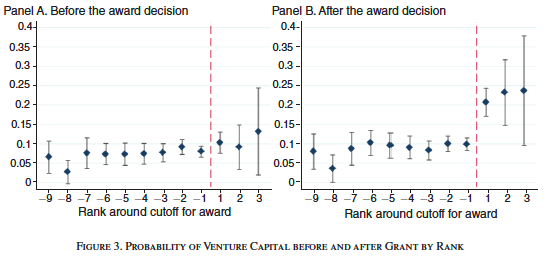
\includegraphics[width=0.7\textwidth, keepaspectratio]{RD_fig.png}
\caption{Reception of venture capital, before and after}
\end{figure}
\begin{example}[Ost, Pan \& Weber, 2018] This paper estimates the return to college using admin data on college enrollment and earnings from Ohio. The running variable here is a GPA, in that this paper uses the fact that colleges dismiss low-performing students on certain GPAs. RDD is used to measure effects of college on earnings. This paper finds that dismissal leads to a short-run increase in earnings and tuition savings, which are wiped out by gains from college graduates 8 years after. They also carry out the test that the result is not driven by manipulation.
\end{example}
\end{mdframed}


\section{Framework}
We will start with a \textbf{sharp RDD}. You can think of this case as a case where the assignment into the treatment is determined by
\[
D_i=1(W_i\geq c(X_i))
\]
where $c(X_i)$ can be a known function of $X_i$ or just a constant. We also keep the potential outcome framework from before, but we will slightly change this to
\begin{align*}
Y_i& = D_iY_i(1)+(1-D_i)Y_i(0)\\
&=Y_i(0)+D_i(Y_i(1)-Y_i(0))\\
&=Y_i(0)+1(W_i\geq c(X_i))\cdot(Y_i(1)-Y_i(0))
\end{align*}
We also keep the regressional framework for the potential outcomes, $Y_i(d)=\mu(X_i,W_i,d)+\epsilon_i(d)$. So we have
\[
E[Y_i(d)|X_i,W_i]=\mu(X_i.W_i.d)
\]
One key assumption that we will carry through this section is the continuity of the conditional expectation on potential outcomes at $W_i=c(X_i)$
\begin{mdframed}[backgroundcolor=blue!5] 
\begin{assumption}[Continuity of $\mu(X_i,W_i,d)$ at $W_i=c$] If $W_i$ has a known cutoff at $c$, we assume that $E[Y_i(1)|X_i, W_i]$ and $E[Y_i(0)|X_i, W_i]$ are continuous around $W_i=c$. Put if differently, 
\[
E[Y_i(d)|X_i, W_i=c^+]=E[Y_i(d)|X_i, W_i=c^-] \ \text{for each } d\in\{0,1\}
\]
\end{assumption}
\end{mdframed}
The above condition also implies that $(\epsilon_i(1), \epsilon_i(0))$ also has a continuous distribution around $W_i=c(X_i)$. If this condition is not satisfied, this implies that there could be more than the $W_i$ variable that jumps around the cutoff, which is what you do not want in an RDD regression.  \par
There is another version of the RDD which is more general than the sharp RDD. A \textbf{fuzzy RDD} setup exploits the jump in the probability of being treated at $W_i=c$. This jump is not necessarily from 0 to 1. Formally, we say we look for discontinuities of 
\[
\Pr(D_i|X_i,W_i)
\]
at $W_i=c(X_i)$. 
\section{Identification in RDD}
We start with a sharp RDD case. Assume that $c(X_i)$ is a constant $c$. We can write
\begin{align*}
E[Y_i|X_i, W_i]&=E[Y_i(0)|X_i, W_i]+E[(Y_i(1)-Y_i(0))1(W_i\geq c(X_i))|X_i, W_i]
\end{align*}
And we can separate the above into two. One with $W_i=c^+$ and the other with $W_i=c^-$.
\begin{align*}
E[Y_i|X_i, W_i=c^+]&=E[Y_i(0)|X_i, W_i=c^+]+E[(Y_i(1)-Y_i(0))|X_i, W_i=c^+]\\
E[Y_i|X_i, W_i=c^-]&=E[Y_i(0)|X_i, W_i=c^-]
\end{align*}
This is because $1(W_i\geq c(X_i))=1$ if $W_i=c^+$ and 0 otherwise. Therefore, 
\begin{align*}
E[Y_i|X_i, W_i=c^+] - E[Y_i|X_i, W_i=c^-]&=E[Y_i(0)|X_i, W_i=c^+]-E[Y_i(0)|X_i, W_i=c^-]\\ &+E[(Y_i(1)-Y_i(0))|X_i, W_i=c^+]
\\&=E[(Y_i(1)-Y_i(0))|X_i, W_i=c^+]
\end{align*}
where the first line on the right hand side vanishes due to the continuity assumptions. Reusing the continuity argument that $E[Y_i(d)|X_i, W_i=c^+]=E[Y_i(d)|X_i, W_i=c^-] \ \text{for each } d\in\{0,1\}$, we can write  
\[
E[(Y_i(1)-Y_i(0))|X_i, W_i=c^+]=E[(Y_i(1)-Y_i(0))|X_i, W_i=c]
\]
Therefore, we have backed out
\[
E[(Y_i(1)-Y_i(0))|X_i, W_i=c]=E[Y_i|X_i, W_i=c^+] - E[Y_i|X_i, W_i=c^-]
\]
which is the average treatment effect at $W_i=c$ and a given $X_i$. This is similar to the LATE in the sense if we let $Z_i=1(W_i\geq c)$, we can get back what is effectively equivalent to the LATE estimator (with the difference in the probability of treatment exactly at 1). Also, we are looking at the treatment effect on the compliers, albeit a very narrow group of people.  \par
For the fuzzy RDD, we can write as follows 
\begin{align*}
E[Y_i|X_i, W_i]&=E[Y_i(0)|X_i, W_i]+E[(Y_i(1)-Y_i(0))\Pr(D_i=1|X_i, W_i)|X_i, W_i]
\end{align*}
So we can do the similar approach as in sharp RDD and get 
\footnotesize{\begin{align*}
E[Y_i|X_i=x, W_i=c^+]&=E[Y_i(0)|X_i=x, W_i=c^+]+\Pr(D_i=1|X_i=x, W_i=c^+)E[Y_i(1)-Y_i(0)|X_i=x, W_i=c^+]\\
E[Y_i|X_i=x, W_i=c^-]&=E[Y_i(0)|X_i=x, W_i=c^-]+\Pr(D_i=1|X_i=x, W_i=c^-)E[Y_i(1)-Y_i(0)|X_i=x, W_i=c^-]
\end{align*}}\normalsize
So using the continuity assumption, the difference in the left hand side can be written as
\footnotesize{\begin{align*}
E[Y_i|X_i=x, W_i=c^+]-E[Y_i|X_i=x, W_i=c^-]&=[\Pr(D_i=1|X_i=x, W_i=c^+)-\Pr(D_i=1|X_i=x, W_i=c^-)]\\
&\times E[Y_i(1)-Y_i(0)|X_i, W_i=c]
\end{align*}}\normalsize
Thus, we also identify an average treatment effect at $W_i=c$ and $X_i=x$, which is now divided by something that is not necessarily 1. 
\[
E[Y_i(1)-Y_i(0)|X_i=x, W_i=c]=\frac{E[Y_i|X_i=x, W_i=c^+]-E[Y_i|X_i=x, W_i=c^-]}{\Pr(D_i=1|X_i=x, W_i=c^+)-\Pr(D_i=1|X_i=x, W_i=c^-)}
\]
\section{Implementation of RDD}
So what can we do in terms of implementing the RDD in practice? One way to implement RDD in practice is to make use of nonparametric regression. The bandwidth, however, should be bounded at $c$. If you are doing a nonparametric regression from the left of the bandwidth, you should apply this on $[c-\epsilon, c)$. For the right hand side, $[c, c+\epsilon]$. If the domain reaches beyond $c$ from either side, there is a huge risk of misfitting the data. While you can do local constant regression in theory, it comes at a huge cost. With this, you can only pin down the level of $Y_i$ from either side. You lose out the rate in which outcome changes within both sides of the boundary. Therefore, if carrying out nonparametric regression, you should do at least a local linear regression. \par
Since we are doing a nonparametric regression, we also run into similar problems as in the typical nonparametric regressions. If you have many other variables to consider, you risk running into the curse of dimensionality. There is also an issue of selecting an optimal bandwidth. We still minimize the AMISE, but at $W_i=c$.  $MSE(h)$ is defined as 
\[
E[(\hat{\mu}(x,c,0)-\mu(x,c,0))^2+(\hat{\mu}(x,c,1)-\mu(x,c,1))^2]
\]
Calonico, Cattaneo, and Tituinik (2014) suggests the use of local quadratic estimator with the optimal bandwidth selected by minimizing above $MSE(h)$ which is typically known as IK bandwidth (Imbens, Kalyanaraman, 2012). Also note that the same trade-off between variance and bias is still in play. \par
There is also a parametric way to implement this as well. One way is to run a separate regression for both left and right of the cutoff. That is, run
\begin{gather*}
Y_i = X_i\beta^- +(c-w_i)X_i\gamma^-+\epsilon_i^-\ \ \text{for }w_i<c\\
Y_i = X_i\beta^+ +(w_i-c)X_i\gamma^++\epsilon_i^+\ \ \text{for }w_i\geq c
\end{gather*}
This setup allows us to fit a different trend on the left and the right of the cutoff $c$. There is also a way in which we make use of both sides of the cutoff. Specifically, we run
\[
Y_i = X_i\beta+ X_i \cdot 1(W_i\geq c)\gamma+X_i\cdot(c-W_i)\delta+X_i\cdot (c-W_i)\cdot 1(W_i\geq c) \mu +\epsilon_i
\]
Here, what happens is that
\begin{itemize}
\item $W_i\geq c$: $Y_i=X_i(\beta+\gamma)+X_i\cdot(c-W_i)(\delta+\mu)$
\item $W_i< c$: $Y_i=X_i(\beta)+X_i\cdot(c-W_i)(\delta)$
\end{itemize}
To make this simple, suppose that $X_i$ is just a vector of 1's. Then, on the $(Y_i, W_i)$ plane,  the jump of the outcome at $W_i=c$ would be captured by the $\gamma$ parameter. Using $\delta, \mu$, we can allow the slopes to differ on either side of the equation. \par
There are some graphical tests that should be carried out. First, we plot $Y_i$ as a function of $W_i$ for a given $X_i$ and see if there is a mean shift. Also, we plot the propensity score $\Pr(D_i=1|X_i, W_i)$ and look for a shift. One thing that should not shift is the distribution of $X_i$'s. So plot $X_i$'s as function of $W_i$ and confirm that there is no shift. Another thing to worry regarding $W_i$ is the possibility of manipulating or gaming. Maybe it might be possible to get into the treatment when you should not be treated (e.g. Ost et al. (2018) checks for this). Therefore, use a McCrary test to confirm that the distribution of $W_i$ do not change at $W_i=c$. \par
Last but not least, what if we do not know the exact cutoff? That is actually not much to worry about, since we can figure out what they might be based on the distribution of $W_i$. Chay, McEwan, and Urquiola (2005) conducts and RDD in the context where the exact cutoffs are unknown using visual evidence. Also, since we lose a lot of data in selecting the optimal bandwidth around the cutoff, RDD is usually poor in terms of external validity.




%%%%%%%%%%%%%%%%%%

\chapter{Introduction to Machine Learning}
\section{Machine Learning}
Machine learning in the context of econometrics is interested in model selection for prediction - finding the parsimonious model in the context of a very large dataset. It ranges from regularized models such as LASSO, Ridge regression, and elastic nets and methods that are much more involved - random forests and neural networks. All of them differ in how they fine-tune the model. \par
\section{Model Selection}
Often, we are interested in controlling a large set of covariates (e.g. propensity score). We can generalize this to the structure where structure refers to specification as well as parameter values. In determining the structure, we face a trade-off: We are tempted to increase the number of covariates since it allows us to fit the data better. However, in doing so, we risk overfitting - the out-sample prediction can perform poorly in terms of variance. Therefore, some method to penalize complexity is required. 
\par
We start with a set $\mathcal{M}$ of candidate models. Then for a model $M\in\mathcal{M}$, we define a penalty parameter $p(M)$ that increases in complexity. Two classical information criteria include
\begin{itemize}
\item Akaike's Information Criterion: Choose $M$ satisfying
\[
\max_{M}\left(\max_\theta \sum_{i=1}^n \log{l_i(\theta;M)}-p(M) \right)
\]
\item Bayesian Information Criterion: Choose $M$ satisfying
\[
\max_{M}\left(\max_\theta \sum_{i=1}^n \log{l_i(\theta;M)}-p(M)\frac{\log{n}}{2} \right)
\]
\end{itemize}
The subtle difference between the two is that BIC tends to be harsher for complexities. This can be seen since for $n>8$, the penalty term is larger. Moreover, the derivation of BIC is based on a Bayesian probabilistic framework - If a selection of candidate models includes a true model for the dataset, then the probability that BIC selects the correct model approaches to 1 as training sample size increases (From Hastie, Tibshirani, Friedman "The Element of Statistical Learning", 2016). Therefore, BIC performs better for selecting the model within the given sample. For out-sample performance, AIC performs better. Both of them, however, can be impractical to calculate when we work with large models. This can be common especially if we allow for multiple levels of interaction between the covariates. In other words, if $p$ is a number of potential covariates, and $n$ is the sample size, we run into the case where $p>>n$. \par
One way out is to penalize complexities with the convex norm penalties. Define
\[
\Vert \theta \Vert _m = \sqrt[m]{\sum_{k=1}^p \vert \theta_k \vert ^m}
\]
and for $m=0$, we have $\Vert \theta \Vert _p=p$, penalties for the two information criteria above. Depending on the selection of $m$, we get different estimators that incorporates different shrinkage mechanisms - Ridge for $m=2$ and LASSO for $m=1$. \par
The general idea of shrinkage is as follows: We know that OLS is BLUE - It has the least variance among the linear, unbiased estimators. But what if we are willing to relax the 'unbiased' condition? Then can we find some estimators that have lower variance and even a lower mean squared error? James, Stein (1961) shows that it is possible and generalizable. \par 
Ridge and LASSO builds upon this idea, but uses different regularization methods. Consider the setup $Y_i=X_i\theta_0+\epsilon_i$. Ridge regression minimizes
\[
\sum_{i=1}^n(Y_i-X_i\theta_0)^2+\lambda\sum_{k=1}^p \theta_k^2 \ \ \left(\sum_{k=1}^p \theta_k^2=\Vert \theta\Vert_2^2\right)
\]
and yields
\[
\hat{\theta} = (X'X+\lambda I_p)^{-1}X'y
\]
Note that as $\lambda$ increases, the $(X'X+\lambda I_p)^{-1}$ term decreases, which drives the coefficients close to 0 and reduce overfitting. With LASSO, the minimization is 
\[
\frac{1}{n}\sum_{i=1}^n(Y_i-X_i\theta_0)^2+\lambda\sum_{k=1}^p |\theta_k| 
\]
and the first order condition can be written as
\[
\frac{2}{n}\sum_i X_{ik}(y_i-X_i\theta)=\lambda s_k, \ \ s_k = \begin{cases}1 & (\hat{\theta}_k>0) \\ -1 & (\hat{\theta}_k<0)\\ [-1,1] & (\hat{\theta}_k=0)\end{cases}
\]
Where $\lambda s_k$ is not necessarily 0, consistent with the idea that we are open to allowing for some bias in order to find an estimator that reduces MSE. 
\par So what is the difference between LASSO and Ridge? Ridge regression drives your coefficients towards 0 but not equal to it. So when it comes to model selection in terms of ruling out irrelevant variables, LASSO does better. This idea is captured by the figure below. As far as computation is concerned, Ridge has a quicker computation speed and works relatively better with multicollinearity.  So the choice of the estimation method depends on your goal of minimizing MSE as well as computation power (but with modern computational power, LASSO is preferred to Ridge). 
\begin{figure}[H]
\centering
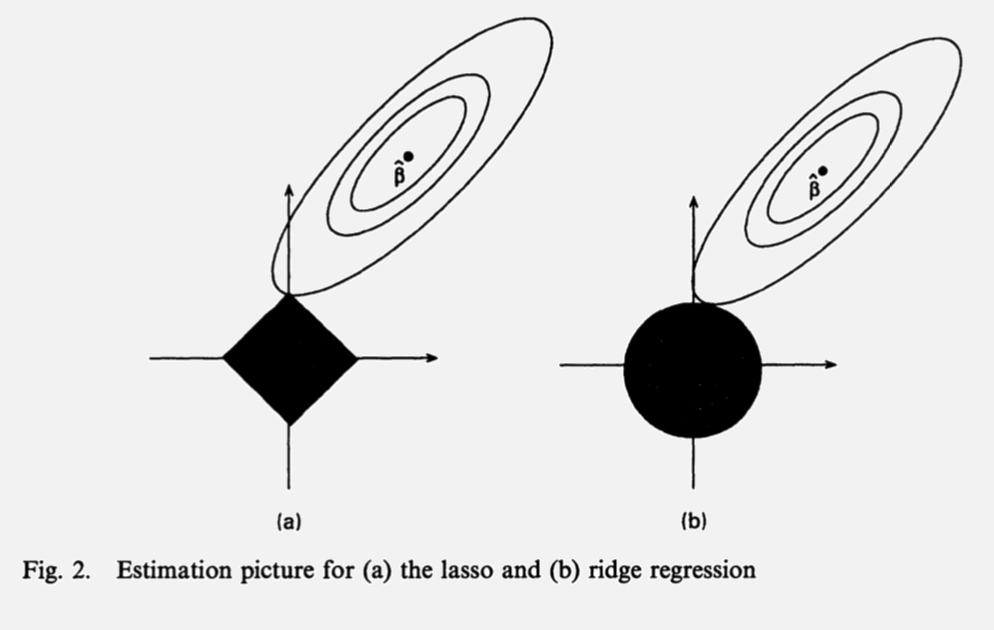
\includegraphics[width=0.67\textwidth, keepaspectratio]{lasso.png}
\caption{Ridge vs LASSO}
\end{figure}
\begin{mdframed}[backgroundcolor=yellow!5] 
\begin{comment}[Can you do both at once?] With \textbf{Elastic Net Regression}, you can. The idea is to use a penalty term that is a convex combination of both $l_1$ and $l_2$ penalty term. Specifically, 
\[
\sum_{i=1}^n(Y_i-X_i\theta_0)^2+\lambda\sum_{k=1}^n\left[\alpha \Vert \theta \Vert_1^2 +(1-\alpha)\Vert \theta \Vert_2^2\right]
\]
If $\lambda=0$ we have an OLS. For $\lambda\neq0$, if $\alpha=1$, we have LASSO, and if $\alpha=0$ we get Ridge. 
\end{comment}
\begin{comment}[Least Angle Regression (LARS)]
The algorithm is as follows
\begin{enumerate}
\item Start with a constant model: For all non-constant covariates, coefficients are 0 and $\lambda=\infty$. 
\item Then, find the covariate that has the largest covariance with the residual. 
\item Change the coefficient for that variable in the same direction as its covariance with the residual ($Y_i- \hat{Y}_i$) until you find a different covariate that has as much covariance with the residuals.  $\lambda$ decrease and $\theta$ is updated along the way.
\item Change the coefficient for the two variables until you find a third variable with the same covariance with the residual. 
\item Stop when all predictors are in the model
\end{enumerate}
When the covariate has the largest covariance with the residual, its angle is smallest. Hence the name LARS. The following figure captures how it works. 
\begin{figure}[H]
\centering
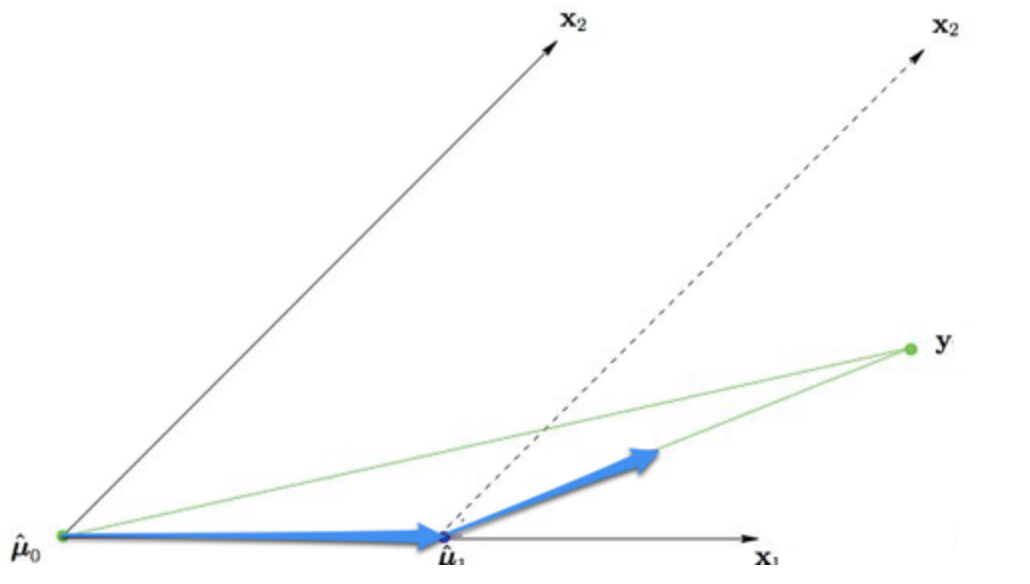
\includegraphics[width=0.67\textwidth, keepaspectratio]{lars.png}
\caption{LARS with two variables}
\end{figure}
\end{comment}
\end{mdframed}
So what is the optimal $\lambda$? It depends on your goal. If your goal is to minimize the prediction error, you can use the following cross-validation methods to come up with one
\begin{itemize}
\item Leave-one-out: Leave one observation out at a time
\item Training vs Test sample: You split the sample into two, build a model given some $\lambda$ and gain prediction error from the test sample. Then, select $\lambda$ minimizing the prediction error there.
\item $K$-fold cross validation:  For $K-1$ blocks, estimate the model given some $\lambda$ and compute the error on the remaining block. Get this for $K$ blocks and compute the average error. Select $\lambda$ minimizing the error. 
\end{itemize}
\section{Some Primer on the Consistency of LASSO}
We want to identify what the true model is in a setting with potentially an infinite number of covariates. To do that, we first set a sparsity assumption, where the number of nonzero coefficients is not too large. As a thought experiment, we increase the number of regressors as $n\to\infty$ in order to approximate the true model. To satisfy the assumption, we require that the number of nonzero regressors to rise at a slower rate than $n$. Specifically, $s_n = o\left(\sqrt{\frac{n}{\log p}}\right)$. \par
If we let $\lambda_n = O\left(\sqrt{\frac{\log p}{n}}\right)$ and have $s_n=o\left(\sqrt{\frac{n}{\log p}}\right)$, then we can show that the prediction error goes to 0 and the LASSO estimator is consistent. Or
\[
\frac{1}{n}\sum_i(X_i\hat{\theta}_n-X_i\hat{\theta}_{0n})^2=O_p(\lambda_n^2s_n)
\]
and 
\[
\Vert \hat{\theta}_n-\hat{\theta}_{0n}\Vert_1 = o_p(\lambda_n s_n) = o_p(1)
\]
This comes at the cost of a slightly slower rate of convergence, which is tolerable as long as it is faster than $n^{-1/4}$.


\section{Random Forests}
Random forests use a series of decision trees - a stack of two-way splits with several number of depths - to solve a classification problem. The splits are based on covariate $k$ being above or below a certain threshold. The process stops at some depth and predict with the mean of $y$ at the terminal node $x$ belongs to. The covariate and the threshold combination that determine the split are selected so as to have the largest separation possible. This is commonly referred to as a `greedy' way of creating random forests.  \par
The detailed way of constructing random forests are as follows. Randomness is injected in several levels: one to select a random sample to train each tree on. Second level of randomness is involved in selecting variable candidates to determine splits for the trees. At the end, we get a prediction for any $x$, average of the predictors of the trees. We can also estimate the prediction error at any observation $x_i$ and gain expected prediction error overall. We can also identify which covariates contributed the most the the prediction using the variance-importance plots. This is where the random forests gain the advantage of interpretability - explaining as to why the results of the prediction came out to be as it is (not just spitting out the number). \par
There are some trade-offs. We want some level of depths in order to reduce the variance in the prediction and get a better fitting. However, too much depth will lead to overfitting. It is usually very difficult to find the happy medium. \par
Below is the example of the decision brought from Varian (2014). A random forests would be obtained by multiple trees, each with different sample (selected through bootstrap) and different variable and threshold combination. 
\begin{figure}[H]
\centering
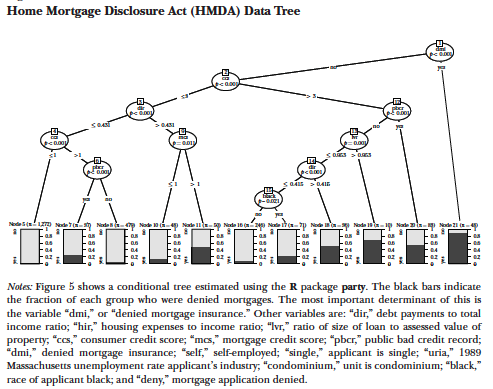
\includegraphics[width=0.7\textwidth, keepaspectratio]{randomforest.png}
\caption{From Varian (2014), Figure 5}
\end{figure}\par
\section{Double Machine Learning De-biasing Technics}
Often we are interested in testing for regarding the value of the parameter of interest. For instance, the average treatment effect under the conditional independence assumption. Specifically, we assume $(\epsilon_i(1),\epsilon_i(0))\perp\!\!\!\perp u_i|X_i$ where $X_i$ contains a large set of covariates. What we may do is to estimate the propensity score using machine learning techniques such as LASSO. Then, estimate the average treatment effect with the formula of our choice. Ideally, we want to conduct some standard tests. \par
Here is the problem - what we have for the propensity score is an estimate with some error. So depending on the size of this error, the estimate of the average treatment effect could be affected. Moreover, the propensity score is just a means towards our ultimate goal of obtaining the average treatment effect - it is merely a nuisance parameter. Since what we are doing involves errors at two different stages, we need a double machine learning de-biasing technics. Specifically, we decouple the propensity score and the treatment effect by applying Neyman Orthogonalization. In principle, what this method allows us to do is to do a two-step estimation by getting the estimate for the propensity score and then estimate the ATE without having to worry too much about the contaminated standard errors originating from the fact that we are not using the exact the propensity score. \par
In our case, what we can do is to
\begin{enumerate}
\item Split data into $K$ folds
\item Use LASSO to estimate $\hat{P}_k=\Pr(D_i=1|X_i)$ in all folds except the $k$th one. $k$ can be from 1 to $K$. 
\item If we are using inverse probability weighting method, for instance, we can get
\[
\widehat{ATE}=\sum_{k=1}^K\left[\frac{\sum_{i\in k}\frac{Y_iD_i}{\hat{P}_k(X_i)}}{\sum_{i\in k}\frac{D_i}{\hat{P}_k(X_i)}}-\frac{\sum_{i\in k}\frac{Y_i(1-D_i)}{1-\hat{P}_k(X_i)}}{\sum_{i\in k}\frac{(1-D_i)}{1-\hat{P}_k(X_i)}}\right]
\]
and use standard asymptotics to conduct tests. 
\end{enumerate}

\end{document}
